\documentclass{article}
\usepackage{tikz}
\usepackage[italian]{babel}
\usepackage{dirtytalk}
\usepackage{amsmath} % for \text
\usepackage{etoolbox} % ifthen
\usepackage[outline]{contour} % glow around text
\usetikzlibrary{calc} % for adding up coordinates
\usetikzlibrary{decorations.markings,decorations.pathmorphing}
\usetikzlibrary{angles,quotes} % for pic (angle labels)
\usetikzlibrary{arrows.meta} % for arrow size
\usepackage{xfp} % higher precision (16 digits?)
\contourlength{1.1pt}

\tikzset{>=latex} % for LaTeX arrow head
\colorlet{myred}{red!85!black}
\colorlet{mydarkred}{red!55!black}
\colorlet{mylightred}{red!85!black!12}
\colorlet{myfieldred}{mydarkred!5} % for S' background
\colorlet{myredhighlight}{myred!20} % highlights simultaneity in ladder paradox
\colorlet{myblue}{blue!80!black}
\colorlet{mydarkblue}{blue!50!black}
\colorlet{mylightblue}{blue!50!black!30}
\colorlet{mylightblue2}{myblue!10}
\colorlet{mygreen}{green!80!black}
\colorlet{mypurple}{blue!40!red!80!black}
\colorlet{mydarkgreen}{green!50!black}
\colorlet{mydarkpurple}{blue!40!red!50!black}
\colorlet{myorange}{orange!40!yellow!95!black}
\colorlet{mydarkorange}{orange!40!yellow!85!black}
\colorlet{mybrown}{brown!20!orange!90!black}
\colorlet{mydarkbrown}{brown!20!orange!55!black}
\colorlet{mypurplehighlight}{mydarkpurple!20} % highlights simultaneity in ladder paradox
\tikzstyle{world line}=[myblue!40,line width=0.3]
\tikzstyle{world line t}=[mypurple!50!myblue!40,line width=0.3]
\tikzstyle{world line'}=[mydarkred!40,line width=0.3]
\tikzstyle{mysmallarr}=[-{Latex[length=3,width=2]},thin]
\tikzstyle{mydashed}=[dash pattern=on 3 off 3]
\tikzstyle{rod}=[mydarkbrown,draw=mydarkbrown,double=mybrown,double distance=2pt,
                 line width=0.2,line cap=round,shorten >=1pt,shorten <=1pt]
%\tikzstyle{rod'}=[rod,draw=mydarkbrown!80!red!85,double=mybrown!80!red!85]
\tikzstyle{vector}=[->,line width=1,line cap=round]
\tikzstyle{vector'}=[vector,shorten >=1.2]
\tikzstyle{particle}=[mygreen,line width=0.9]
\tikzstyle{photon}=[-{Latex[length=5,width=4]},myorange,line width=0.8,decorate,
                    decoration={snake,amplitude=1.0,segment length=5,post length=5}]

\def\tick#1#2{\draw[thick] (#1) ++ (#2:0.06) --++ (#2-180:0.12)}
\def\tickp#1#2{\draw[thick,mydarkred] (#1) ++ (#2:0.06) --++ (#2-180:0.12)}
\def\Nsamples{100} % number samples in plot







\usepackage[letterpaper,top=2cm,bottom=2cm,left=3cm,right=3cm,marginparwidth=1.75cm]{geometry}


\usepackage{physics}
\usepackage{amsmath}
\usepackage{bbold}
\usepackage{dsfont}
\usepackage{amsthm}
\usepackage{mathtools}
\usepackage{amssymb}
\usepackage{tensor}
\numberwithin{equation}{section}
\numberwithin{equation}{subsection}

\pagenumbering{Roman}

\usepackage{graphicx}
\usepackage{subfig}
\usepackage{float}

\usepackage[colorlinks=true, allcolors=blue]{hyperref}

\setcounter{page}{0}
\title{\textbf{Introduzione a Temi e Modelli della Fisica Teorica}}
\author{Samuele Pettinotti, Alessio Belshi}

\begin{document}
\maketitle

\newpage

\tableofcontents
\newpage

\pagenumbering{arabic}
\input{Sezioni/1.Relatività_Ristretta}
\newpage

\section{Elettromagnetismo}\label{sec:2}
\subsection{Forza di Lorentz}\label{sec:2.1}
Alla luce di quanto detto alla fine della sezione \ref{sec:1.6} possiamo studiare la dinamica di una particella carica sottoposta ad un campo elettromagnetico. Dunque, nel caso considerato, il principio di inerzia \eqref{eq:princ_iner} e il teorema delle forze vive \eqref{eq:teo_for_vive} saranno della forma:

\begin{equation}
    \begin{cases}
    \dfrac{d\Vec{p}}{dt}=\Vec{F}=e\Vec{E}+\dfrac{e}{c}\Vec{v}\times \Vec{B}
    \\
    \\
    \dfrac{dE}{dt}=\Vec{F}\Vec{v}=e\Vec{E}\Vec{v}
    \end{cases}\, \footnote{Nella seonda equazione consideriamo solo il primo termine della forza poiché il secondo non fa lavoro.}
\end{equation}
vogliamo riscrivere queste quattro equazioni in forma covariante.
Consideriamo il principio di inerzia ed introduciamo il tempo proprio mediante la regola della catena:
\begin{equation}  
    \dfrac{d\Vec{p}}{ds}\dfrac{ds}{dt}=\left[e\Vec{E}+\dfrac{e}{c}\Vec{v}\times \Vec{B}  \implies \dfrac{d\Vec{p}}{ds}=e\Vec{E}+\dfrac{e}{c}\Vec{v}\times \Vec{B}\right]\dfrac{dt}{ds}
\end{equation}
consideriamo la definizione di quadrimpulso \eqref{eq:def_quadimpul} (in particolare la parte spaziale) e scomponiamo nelle tre componenti, esaminiamo lo per x:
\begin{equation}  
    \dfrac{dp_x}{ds}=mc \dfrac{du^1}{ds}=e\left[E_1+\dfrac{1}{c}(v_2B_3-v_3B_2)\right] \dfrac{dt}{ds}
\end{equation}
Esaminiamo i seguenti termini
\begin{equation}
    \begin{gathered}
      \dfrac{dt}{ds}=\dfrac{c}{c}\dfrac{dt}{ds}=\dfrac{dx^0}{cds}=\dfrac{u^0}{c}
      \\
\Vec{v}\dfrac{dt}{ds}=\dfrac{d\Vec{x}}{dt}\dfrac{dt}{ds}=\dfrac{d\Vec{x}}{ds}=\Vec{u}
\end{gathered}
\end{equation}
sostituendo nella precedente, otteniamo:
\begin{equation}  \label{eq:quadfor_Lorentz_1}
    \begin{gathered}
    \dfrac{dp_x}{ds}=mc \dfrac{du^1}{ds}=\dfrac{e}{c}(u^0E_1+ u^2B_3-u^3B_2)
    \\
    \qquad \vdots
     \end{gathered}
\end{equation}
Ora, consideriamo il teorema delle forze vive  e procediamo similmente:
\begin{equation}
\begin{gathered}\label{eq:quadfor_Lorentz_2}
  \dfrac{d}{dt}\left(\dfrac{mc^2}{\sqrt{1-\dfrac{v^2}{c^2}}}\right)=e(E_1v_1+E_2v_2+E_3v_3)
  \\
  mc^2\dfrac{d}{ds}(\gamma)=e(E_1v_1+E_2v_2+E_3v_3)\dfrac{dt}{ds}
  \\
  mc\dfrac{d}{ds}\left(\dfrac{cdt}{ds}\right)=\dfrac{e}{c}(E_1u^1+E_2u^2+E_3u^3) \implies mc\dfrac{du^0}{ds}=\dfrac{e}{c}(E_1u^1+E_2u^2+E_3u^3) 
\end{gathered}
\end{equation}
Considerando la proprietà di abbassamento di indice:
\begin{equation*}
u^\alpha=(u^0,\Vec{u}) \rightarrow u_\alpha=(u^0,-\Vec{u})
\end{equation*}
applicandola alle relazioni \eqref{eq:quadfor_Lorentz_1} e \eqref{eq:quadfor_Lorentz_2}, otteniamo:
\begin{equation}
    \begin{cases}
     mc\dfrac{du^0}{ds}=-\dfrac{e}{c}(E_1u_1+E_2u_2+E_3u_3) 
    \\
    mc \dfrac{du^1}{ds}=\dfrac{e}{c}(u^0E_1 -u_2B_3+u_3B_2)
    \\
    mc \dfrac{du^2}{ds}=\dfrac{e}{c}(u^0E_2 -u_3B_1+u_1B_3)
    \\
    mc \dfrac{du^3}{ds}=\dfrac{e}{c}(u^0E_3 -u_1B_2+u_2B_1)
    \end{cases}\, 
\end{equation}
Adesso definiamo un nuovo oggetto, che chiamiamo \textit{tensore del campo elettromagnetico}, il quale soddisfi la: 
\begin{equation}\label{eq:dinam_parti}
    mc\dfrac{du^\alpha}{ds}=\dfrac{e}{c}F\indices{^{\alpha\beta}}u_\beta
\end{equation}
in particolare, abbiamo:
\begin{equation}
F\indices{^{\alpha\beta}}=
\begin{pmatrix}
  0 & -E_x & -E_y & -E_z  \\
  E_x & 0 & -B_z & B_y  \\
  E_y & B_z & 0 & -B_x  \\
  E_z & -B_y & B_x & 0
\end{pmatrix}
\end{equation}
è, evidentemente, un tensore antisimmetrico che ha sei componenti indipendenti, le tre componenti del campo elettrico e le tre componenti del campo magnetico.

In linea di principio possiamo, facilmente, esprimere la dinamica della particella in ogni sistema di riferimento inerziale secondo la trasformazione:

\begin{equation} \label{eq:tras_F}
    F\indices{^{\alpha\beta}}
   \xrightarrow[\text{}]{\text{L}}
    F\indices{^'^{\alpha\beta}}
    =\Lambda\indices{^\alpha_\mu}
    \Lambda\indices{^\beta_\nu}
    F\indices{^{\mu\nu}}
\end{equation}

Consideriamo il caso semplice di un boost lungo l'asse x, quindi la matrice associata alla trasformazione sarà:
\begin{equation}
\Lambda(\beta)=
\begin{pmatrix}
\gamma & -\gamma\beta & 0 & 0   \\
 -\gamma\beta &\gamma & 0 & 0    \\
  0 & 0 & 1 & 0                   \\
  0 & 0 & 0 & 1
\end{pmatrix}
\end{equation}
Allora seguendo la trasformazione \eqref{eq:tras_F} avremo le componenti nel sistema primato:
\begin{equation*}
    \begin{split}
         F\indices{^'^{01}}=-E\indices{^'_x}
    &=
    \Lambda\indices{^0_\mu}
    \Lambda\indices{^1_\nu}
    F\indices{^{\mu\nu}}=\Lambda\indices{^0_0}
    \Lambda\indices{^1_\nu}
    F\indices{^{0\nu}}+\Lambda\indices{^0_1}
    \Lambda\indices{^1_\nu}
    F\indices{^{1\nu}}=\gamma
    \Lambda\indices{^1_\nu}
    F\indices{^{0\nu}}-\gamma\beta
    \Lambda\indices{^1_\nu}
    F\indices{^{1\nu}}
    \\
    &=\gamma
    \Lambda\indices{^1_0}
    F\indices{^{00}}+\gamma
    \Lambda\indices{^1_1}
    F\indices{^{01}}-\gamma\beta
    \Lambda\indices{^1_0}
    F\indices{^{10}}-\gamma\beta
    \Lambda\indices{^1_1}
    F\indices{^{11}}=
    -\gamma^2
   E_x+(\gamma\beta)^2E_x=-E_x
    \end{split}
\end{equation*}
\begin{equation*}
    \begin{split}
         F\indices{^'^{02}}=-E\indices{^'_y}
    &=
    \Lambda\indices{^0_\mu}
    \Lambda\indices{^2_\nu}
    F\indices{^{\mu\nu}}=\Lambda\indices{^0_0}
    \Lambda\indices{^2_\nu}
    F\indices{^{0\nu}}+\Lambda\indices{^0_1}
    \Lambda\indices{^2_\nu}
    F\indices{^{1\nu}}=\gamma
    \Lambda\indices{^2_\nu}
    F\indices{^{0\nu}}-\gamma\beta
    \Lambda\indices{^2_\nu}
    F\indices{^{1\nu}}
    \\
    &=\gamma
    \Lambda\indices{^2_2}
    F\indices{^{02}}-\gamma\beta
    \Lambda\indices{^2_2}
    F\indices{^{12}}=-\gamma
   E_y+\gamma\beta B_z=-\gamma( E_y-\beta B_z)
    \end{split}
\end{equation*}
sviluppando tutte le componenti arriviamo alle trasformazioni: 
\begin{equation}
    \begin{cases}
    E\indices{^'_x}=E_x
    \\
    E\indices{^'_y}=\dfrac{E_y-\dfrac{v}{c}B_z}{\sqrt{1-\dfrac{v^2}{c^2}}}
    \\
     E\indices{^'_z}=\dfrac{E_z+\dfrac{v}{c}B_y}{\sqrt{1-\dfrac{v^2}{c^2}}}
    \end{cases}\,
  \begin{cases}
   B\indices{^'_x}=B_x
    \\
    B\indices{^'_y}=\dfrac{B_y+\dfrac{v}{c}E_z}{\sqrt{1-\dfrac{v^2}{c^2}}}
    \\
     B\indices{^'_z}=\dfrac{B_z-\dfrac{v}{c}E_y}{\sqrt{1-\dfrac{v^2}{c^2}}}
    \end{cases}\,
\end{equation}
Se invece consideriamo un moto la cui velocità ha direzione arbitraria, possiamo scomporre i campi nelle componenti parallele e perpendicolari alla direzione di moto:
\begin{equation*}
    \Vec{E}=\Vec{E_\parallel}+\Vec{E_\perp} \quad \text{ove}
    \qquad\Vec{E_\parallel}=\dfrac{\Vec{E}\Vec{\beta}}{\beta}\dfrac{\Vec{\beta}}{\beta}\quad\text{e}\quad
    \Vec{E_\perp}=\Vec{E}-\Vec{E_\parallel}
\end{equation*}
quindi le componenti si trasformano secondo le
\begin{equation}
    \begin{cases}
    E\indices{^'_\parallel}=E_\parallel
    \\
    E\indices{^'_\perp}=\dfrac{\Vec{E_\perp}+\Vec{\beta}\times\Vec{B}}{\sqrt{1-\dfrac{v^2}{c^2}}}
    \end{cases}\,
  \begin{cases}
   B\indices{^'_\parallel}=B_\parallel
    \\
    B\indices{^'_\perp}=\dfrac{B_\perp-\Vec{\beta}\times\Vec{E}}{\sqrt{1-\dfrac{v^2}{c^2}}}
    \end{cases}\,
\end{equation}
per una trasformazione generica le componenti della matrice sono \eqref{eq:generic_elem_tras}, le equazioni dei campi diventano:
\begin{equation}\label{eq:Campi_genric}
    \Vec{E'}=\gamma(\Vec{E}+\Vec{\beta}\times\Vec{B})-\dfrac{(\gamma -1)}{\beta^2}(\Vec{E}\Vec{\beta})\Vec{\beta} \qquad \Vec{B'}=\gamma(\Vec{B}-\Vec{\beta}\times\Vec{E})-\dfrac{(\gamma -1)}{\beta^2}(\Vec{B}\Vec{\beta})\Vec{\beta}
\end{equation}
Consideriamo, ora, il caso prototipo della relatività ristretta (Fig.\ref{fig:TL}), in particolare nel sistema $S$ i campi valgano $\Vec{E}=0$ e $\Vec{B}\neq0$, quindi nel sistema $S'$ avremo $\Vec{E'}=\gamma\Vec{\beta}\times\Vec{B}$ e $\Vec{B'}=\gamma\Vec{B}$. Allora dalla relazione \eqref{eq:Campi_genric} possiamo scrivere:\begin{equation*}
    \gamma\Vec{B}=\Vec{B'}+\dfrac{(\gamma -1)}{\beta^2}(\Vec{B}\Vec{\beta})\Vec{\beta}
\end{equation*}
sostituendo  nel campo elettrico:
\begin{equation*}
    \Vec{E'}=\Vec{\beta}\times\left(\Vec{B'}+\dfrac{(\gamma -1)}{\beta^2}(\Vec{B}\Vec{\beta})\Vec{\beta}\right)=\Vec{\beta}\times\Vec{B'}
\end{equation*}
procedendo in questa maniera abbiamo dimostrato che se $\Vec{E}$, $\Vec{B}$ e $\Vec{\beta}$ (ossia la direzione di propagazione) sono ortogonali in un sistema di riferimento, allora lo saranno \textit{in ogni altro}.\footnote{Similmente, si può verificare il caso in cui $\Vec{E}\neq0$, $\Vec{B}=0$, ottenendo$\Vec{B'}=-\Vec{\beta}\times\Vec{E'}$}

Ci chiediamo se, a partire da $\Vec{E}$ e $\Vec{B}$, possiamo costruire delle quantità scalari\footnote{Ci interessano, per le ovvie proprietà Lorentz invarianti.}.
Con questo scopo consideriamo le proprietà di abbassamento ed innalzamento di indice sul tensore elettromagnetico
\begin{equation}\phantomsection\label{eq:scalar_mod}
F\indices{_{\alpha\beta}}=\eta\indices{_{\alpha\mu}} \eta\indices{_{\beta\nu}}F\indices{^{\mu\nu}}=
\begin{pmatrix}
  0 & E_x & E_y & E_z  \\
  -E_x & 0 & -B_z & B_y  \\
  -E_y & B_z & 0 & -B_x  \\
  -E_z & -B_y & B_x & 0
\end{pmatrix}
\end{equation}
avremo, quindi, la quantità scalare:
\begin{equation}
    F\indices{_{\alpha\beta}}F\indices{^{\alpha\beta}}=-2(E^2-B^2)
    \end{equation}
Possiamo definire un altro scalare a partire dal \textit{duale del tensore elettromagnetico} definito come:
\begin{equation}
    F\indices{^{*\mu\nu}}=\dfrac{1}{2}\epsilon\indices{^{\mu\nu\rho\sigma}} F\indices{_{\rho\sigma}}=\begin{pmatrix}
  0 & -B_x & -B_y & -B_z  \\
  B_x & 0 & E_z & -E_y  \\
  B_y & -E_z & 0 & E_x  \\
  B_z & E_y & -E_x & 0
\end{pmatrix}
\end{equation}
lo scalare sarà quindi:
\begin{equation}\phantomsection\label{eq:scalar_prod}
    F\indices{^{*\alpha\beta}}F\indices{_{\alpha\beta}}=-4\Vec{E}\Vec{B}
    \end{equation}
    Notiamo che se $\Vec{E}\Vec{B}=0$ i campi saranno $\Vec{E}\perp\Vec{B}$, essendo uno scalare i campi saranno perpendicolari in ogni sistema di rifermento. Inoltre potrò sempre trovare un sistema primato nel quale il modulo di $E'$ o di $B'$ sarà nullo.

  Dopo queste definizioni fondamentali torniamo ad analizzare la dinamica della particella sottoposta ad un campo elettromagnetico che, ricordiamo, essere descritta dalla \eqref{eq:dinam_parti}. In particolare la risolveremo in alcuni casi notevoli. 
  Consideriamo un primo caso nel quale ci sia solo un campo elettrico e quest'ultimo abbia direzione e verso $\Vec{E}\parallel\Vec{x}$. Quindi avremo che $F\indices{^{01}}=-F\indices{^{10}}=-E_x=-E$. Ponendo $\alpha=0$ l'equazione della dinamica diventa:
  \begin{equation}
    mc\dfrac{du^0}{ds}=\dfrac{e}{c}F\indices{^{0\beta}}u_\beta=\dfrac{e}{c}F\indices{^{01}}u_1=-\dfrac{e}{c}Eu_1=\dfrac{e}{c}Eu^1
\end{equation}
dove nell'ultimo passaggio abbiamo alzato l'indice e cambiato di segno.
Se, invece, poniamo $\alpha=1$, otteniamo: 
\begin{equation}
    mc\dfrac{du^1}{ds}=\dfrac{e}{c}F\indices{^{1\beta}}u_\beta=\dfrac{e}{c}F\indices{^{10}}u_0=\dfrac{e}{c}Eu_0=\dfrac{e}{c}Eu^0
\end{equation}
in questo caso il cambio di segno non avviene poiché si ha un termine non spaziale. Mentre per $\alpha=2,3$ i termini sono nulli, quindi nel caso in cui la particella avesse avuto velocità iniziali lungo $y$ e $z$ diverse da zero, solo rispetto a suddette direzioni, il moto risulta rettilineo uniforme. Definendo $g=\dfrac{eE}{mc^2}$ otteniamo il sistema:
\begin{equation}
   \begin{cases}
    \dfrac{du^o}{ds}=gu^1=\omega^0
    \\
    \\
    \dfrac{du^1}{ds}=gu^0=\omega^1
      \end{cases}
\end{equation}
che riconosciamo essere le equazioni di un moto uniformemente accelerato $(\omega^0)^2-(\omega^1)^2=-g^2$. Le soluzioni del sistema saranno quelle di Rindler \eqref{eq:solu_rindler}, che nel caso seguente assumono la forma particolare 
\begin{equation}
   \begin{cases}
      x^0=\dfrac{1}{g}\sinh{gs}
      \\
      \\
     x^1=\dfrac{1}{g}\cosh{gs}
      \end{cases}\, 
\end{equation}.

 Consideriamo il secondo caso nel quale ci sia solo un campo magnetico e quest'ultimo abbia direzione e verso $\Vec{B}\parallel\Vec{x}$. Quindi avremo che $F\indices{^{23}}=-F\indices{^{32}}=-B_x=-B$. Ponendo $\alpha=2$, L'equazione della dinamica diventa:
  \begin{equation}
    mc\dfrac{du^2}{ds}=\dfrac{e}{c}F\indices{^{2\beta}}u_\beta=\dfrac{e}{c}F\indices{^{23}}u_3=-\dfrac{e}{c}Bu_3=\dfrac{e}{c}Bu^3
\end{equation}
Se, invece, poniamo $\alpha=3$, otteniamo: 
\begin{equation}
    mc\dfrac{du^3}{ds}=\dfrac{e}{c}F\indices{^{3\beta}}u_\beta=\dfrac{e}{c}F\indices{^{32}}u_2=\dfrac{e}{c}Bu_2=-\dfrac{e}{c}Bu^2
\end{equation}
Mentre per $\alpha=0,1$ i termini sono tutti nulli, quindi, come nel caso precedente, le componenti della velocità si conservano. Definendo $g=\dfrac{eB}{mc^2}$ otteniamo il sistema:
\begin{equation}
   \begin{cases}
    \dfrac{du^2}{ds}=gu^3=g\dfrac{dz}{ds}
    \\
    \\
    \dfrac{du^3}{ds}=-gu^2=-g\dfrac{dy}{ds}
      \end{cases}
\end{equation}
nella la prima equazione, considerando la definizione della quadrivelocità, otteniamo:
\begin{equation}
   \dfrac{d}{ds}\dfrac{dt}{ds}\dfrac{dy}{dt}=g\dfrac{dt}{ds}\dfrac{dz}{dt} \implies \dfrac{dv_y}{ds}=gv_z
   \end{equation}
   facendo lo stesso anche per la seconda equazione il sistema assume la forma:
   \begin{equation}
   \begin{cases}
    \dfrac{dv_y}{ds}=gv_z
    \\
    \\
 \dfrac{dv_z}{ds}=-gv_y
      \end{cases}
      \implies
       \begin{cases}
    \dfrac{d^2v_y}{{ds}^2}=-g^2v_y
    \\
    \\
   \dfrac{d^2v_z}{{ds}^2}=-g^2v_z
 \end{cases}
\end{equation}
Possiamo riconoscere nell'ultimo sistema una forma assai simile ad un oscillatore armonico. Le soluzioni saranno perciò della forma ben nota:\begin{equation}
   \begin{cases}
   v_y=A\cos{gt}+B\sin{gt}
    \\
   v_z=-A\sin{gt}+B\cos{gt}
      \end{cases}\footnote{La determinazione delle costanti avviene, come nella sezione \ref{sec:1.7}, attrverso le equazioni $\dfrac{dv_y}{ds}=gv_z$}
\end{equation}
Concludiamo che la composizione del moto rettilineo uniforme lungo $x$ e del moto circolare nel piano $y-z$ forma un moto elicoidale.

\subsection{Sorgenti elettromagnetiche}\label{sec:2.2}
Consideriamo un insieme di $n$ particelle cariche, con carica generica $e_n$, che seguono traiettorie $x_n(t)$ arbitrarie determinate dall'interazione reciproca. Definiamo la \textit{densità di carica} come:
\begin{equation}\phantomsection\label{eq:Def_dens_carica}
    \rho(t,\Vec{x})=\sum_n e_n  \delta^3(\Vec{x}-\Vec{x}_n)
\end{equation}
ove $\delta^3(\Vec{x}-\Vec{x_n})$ è la \textit{delta di Dirac} definita nello spazio tridimensionale. Tale definizione di densità di carica è consistente con l'intuizione fisica, in quanto: la densità sarà nulla laddove la particella non è presente ed infinita dove la particella è localizzata.\footnote{Ovviamente l'integrale sullo spazio delle configurazioni di $\rho$ restituisce la carica in virtù della proprietà di normalizzazione della delta di Dirac.}
 Definiamo la \textit{densità di corrente} come:
\begin{equation}\phantomsection\label{eq:Def_dens_corr}
    \Vec{j}(t,\Vec{x})=\sum_n e_n  \delta^3(\Vec{x}-\Vec{x}_n)\dfrac{d\Vec{x_n}}{dt}
\end{equation}
ove $\dfrac{d\Vec{x_n}}{dt}$ non è altro che la velocità della particella.

Definendo $j^0=c\rho$ e $x\indices{^0_n}=ct$, posso scrivere una relazione che unifichi le due densità:
\begin{equation}
    j^\alpha(t,\Vec{x})=\sum_n e_n  \delta^3(\Vec{x}-\Vec{x}_n)\dfrac{dx\indices{^\alpha_n}}{dt}
\end{equation}
in quest'ultima relazione non è immediato riconoscere un quadrivettore, poiché la derivata temporale è una velocità in senso classico che non si trasforma come un tensore. Per palesare la sua natura tensoriale, quello che facciamo è usare la proprietà di normalizzazione della delta:
\begin{equation}\phantomsection\label{eq:def_quad_corr1}
    j^\alpha(t,\Vec{x})=\int dt'\delta(t-t')\sum_n e_n  \delta^3(\Vec{x}-\Vec{x}_n)\dfrac{dx\indices{^\alpha_n}}{dt'}
\end{equation}
ricordando la proprietà della delta $\delta(ax)=\dfrac{\delta(x)}{|a|}$ ed introducendo la delta di Dirac quadridimensionale $\delta^4(x^\mu-x\indices{^{'\mu}})=\delta(ct-ct')\delta^3(\Vec{x}-\Vec{x'})$ posso riscrivere la \eqref{eq:def_quad_corr1} come:
\begin{equation}\phantomsection\label{eq:def_quad_corr2}
    \begin{split}
        j^\alpha(t,\Vec{x})&=c\int dt'\delta^4(x^\mu-x\indices{_n^{\mu}})\sum_n e_n \dfrac{dx\indices{^\alpha_n}}{dt'}\\
        &=c\int \dfrac{dt'}{ds}ds\delta^4(x^\mu-x\indices{_n^{\mu}})\sum_n e_n  \dfrac{dx\indices{^\alpha_n}}{ds}\dfrac{ds}{dt'}\\
        &=c\int ds\delta^4(x^\mu-x\indices{_n^{\mu}})\sum_n e_n \dfrac{dx\indices{^\alpha_n}}{ds}
    \end{split}
    \end{equation}
a questo punto siamo in grado di dire che $j^\alpha$ è un quadrivettore poiché dipende dalla quadrivelocità. Quindi varrà la consueta proprietà di trasformazione \eqref{eq:tras_generic}.

Partendo dalle \eqref{eq:Def_dens_carica}, \eqref{eq:Def_dens_corr} consideriamo la divergenza di $\Vec{j}$:
\begin{equation}
    \Vec{\nabla}\Vec{j}=\sum_{i=1}^3\sum_n e_n\left[\dfrac{\partial}{\partial x^i}\delta^3(\Vec{x}-\Vec{x}_n)\right]  \dfrac{dx\indices{_n^i}}{dt}
\end{equation}
Tenendo presente che se una funzione ha una dipendenza del tipo $F(x-y)$, allora vale l'identità $\dfrac{\partial F}{\partial x}=-\dfrac{\partial F}{\partial y}$. Possiamo riscrivere, sottintendendo la sommatoria, la divergenza come:
\begin{equation}
\begin{split}
    \Vec{\nabla}\Vec{j}&=-\sum_n e_n\left[\dfrac{\partial}{\partial x\indices{_n^i}}\delta^3(\Vec{x}-\Vec{x}_n)\right] \dfrac{dx\indices{_n^i}}{dt}\\
    &=-\dfrac{\partial}{\partial t}\sum_n \delta^3(\Vec{x}-\Vec{x}_n) e_n\\
    &=-\dfrac{\partial}{\partial t} \rho 
    \end{split}
\end{equation}
notiamo che abbiamo potuto portare dentro la derivazione temporale il termine $e_n$ poiché le cariche sono indipendenti dal tempo.
Otteniamo così un'\textit{equazione di continuità}:
\begin{equation}\phantomsection\label{eq:eq_cont_elett}
    \Vec{\nabla}\Vec{j}+\dfrac{\partial}{\partial t} \rho =0
\end{equation}
Nel formalismo tensoriale avevamo già trovato la relazione \eqref{eq:eq_cont}, quindi concludiamo:
\begin{equation}
    \partial_\alpha j^\alpha=\Vec{\nabla}\Vec{j}+\dfrac{\partial}{\partial t} \rho =0
\end{equation}
L'importanza del quadrivettore $j^\alpha=(c\rho,\Vec{j})$ che abbiamo creato consiste nella sua rappresentazione delle sorgenti elettromagnetiche.

\subsection{Equazioni di Maxwell}\label{sec:2.3}
Dagli studi passati sappiamo che le \textit{equazioni di Maxwell}, nella loro forma differenziale, si presentano come:
\begin{equation}
\begin{cases}
  \Vec{\nabla}\cdot\Vec{E}=4\pi\rho\\ 
  \Vec{\nabla}\times\Vec{B}-\dfrac{1}{c}\dfrac{\partial\Vec{E}}{\partial t}=\dfrac{4\pi}{c}\Vec{j}
    \\
    \Vec{\nabla}\cdot\Vec{B}=0 \\
  \Vec{\nabla}\times\Vec{E}+\dfrac{1}{c}\dfrac{\partial\Vec{B}}{\partial t} =0
\end{cases}
\end{equation}
ove le prime due sono non omogenee e sono dette, rispettivamente, \textit{legge di Gauss} e \textit{legge di Ampère-Maxwell}. Le ultime due, invece, sono omogenee e sono dette \textit{legge dell'inesistenza di monopoli magnetici} e \textit{legge di Faraday}.
Vogliamo, ora, riformularle secondo il formalismo tensoriale, procediamo con ordine.

\textbf{Legge di Gauss}

Sviluppiamo la divergenza e sostituiamo le componenti con i termini tensoriali adeguati, inoltre sappiamo che $\dfrac{\partial F\indices{^{00}}}{\partial x^0}=0$, quindi:
\begin{equation*}
    \Vec{\nabla}\cdot\Vec{E}=\dfrac{\partial E_x}{\partial x}+\dfrac{\partial E_y}{\partial y}+\dfrac{\partial E_z}{\partial z}=\dfrac{\partial F\indices{^{10}}}{\partial x^1}+\dfrac{\partial F\indices{^{20}}}{\partial x^2}+\dfrac{\partial F\indices{^{30}}}{\partial x^3}=\dfrac{\partial F\indices{^{10}}}{\partial x^1}+\dfrac{\partial F\indices{^{20}}}{\partial x^2}+\dfrac{\partial F\indices{^{30}}}{\partial x^3}+\dfrac{\partial F\indices{^{00}}}{\partial x^0}=\dfrac{\partial F\indices{^{\mu0}}}{\partial x^\mu}
\end{equation*} 
mentre la parte destra dell'equazione la riscriviamo:
\begin{equation*}
    4\pi\rho=\dfrac{4\pi}{c}j^0
\end{equation*} 
concludendo che:
\begin{equation}\phantomsection\label{eq:leg_gauss}
    \dfrac{\partial F\indices{^{\mu0}}}{\partial x^\mu}=4\pi j^0
\end{equation} 

\textbf{Legge di Ampère-Maxwell}

Scomponiamo la relazione vettoriale nelle componenti, in particolare consideriamo la x.
\begin{equation*}
   \dfrac{\partial B_z}{\partial y}-\dfrac{\partial B_y}{\partial z}-\dfrac{1}{c}\dfrac{\partial E_x}{\partial t}=\dfrac{\partial F\indices{^{21}}}{\partial x^2}+\dfrac{\partial F\indices{^{31}}}{\partial x^3}+\dfrac{\partial F\indices{^{01}}}{\partial x^0}=\dfrac{\partial F\indices{^{21}}}{\partial x^2}+\dfrac{\partial F\indices{^{31}}}{\partial x^3}+\dfrac{\partial F\indices{^{01}}}{\partial x^0}+\dfrac{\partial F\indices{^{11}}}{\partial x^1}=\dfrac{\partial F\indices{^{\mu1}}}{\partial x^\mu}
\end{equation*}
mentre la parte destra sarà banalmente:
\begin{equation*}
    \dfrac{4\pi}{c}j^1
\end{equation*}
considerando, ora, tutte le componenti di $i=1,2,3$ otteniamo:
\begin{equation}\phantomsection\label{eq:leg_am-ma}
    \dfrac{\partial F\indices{^{\mu i}}}{\partial x^\mu}=\dfrac{4\pi}{c}j^i
\end{equation} 

\textbf{Legge dell'inesistenza dei monopoli magnetici}

Sviluppiamo la divergenza e sostituiamo le componenti con i termini tensoriali adeguati, inoltre sappiamo che $\dfrac{\partial F\indices{^{*00}}}{\partial x^0}=0$, quindi:
\begin{equation*}
    \Vec{\nabla}\cdot\Vec{B}=\dfrac{\partial B_x}{\partial x}+\dfrac{\partial B_y}{\partial y}+\dfrac{\partial B_z}{\partial z}=\dfrac{\partial F\indices{^{*10}}}{\partial x^1}+\dfrac{\partial F\indices{^{*20}}}{\partial x^2}+\dfrac{\partial F\indices{^{*30}}}{\partial x^3}=\dfrac{\partial F\indices{^{*10}}}{\partial x^1}+\dfrac{\partial F\indices{^{*20}}}{\partial x^2}+\dfrac{\partial F\indices{^{*30}}}{\partial x^3}+\dfrac{\partial F\indices{^{*00}}}{\partial x^0}=0
\end{equation*} 
concludiamo che:
\begin{equation}\phantomsection\label{eq:leg_mono}
    \dfrac{\partial F\indices{^{*\mu0}}}{\partial x^\mu}=0
\end{equation}


\textbf{Legge di Faraday}

Scomponiamo la relazione vettoriale nelle componenti, in particolare consideriamo la x.
\begin{equation*}
\begin{aligned}
   \dfrac{\partial E_z}{\partial y}-\dfrac{\partial E_y}{\partial z}+\dfrac{1}{c}\dfrac{\partial B_x}{\partial t}&=\dfrac{\partial F\indices{^{*12}}}{\partial x^2}+\dfrac{\partial F\indices{^{*13}}}{\partial x^3}+\dfrac{\partial F\indices{^{*10}}}{\partial x^0}=\dfrac{\partial F\indices{^{*12}}}{\partial x^2}+\dfrac{\partial F\indices{^{*13}}}{\partial x^3}+\dfrac{\partial F\indices{^{*10}}}{\partial x^0}+\dfrac{\partial F\indices{^{*11}}}{\partial x^1}\\
   &=\dfrac{\partial F\indices{^{*1\mu}}}{\partial x^\mu}=-\dfrac{\partial F\indices{^{*\mu1}}}{\partial x^\mu}=0
   \end{aligned}
\end{equation*}
considerando, ora, tutte le componenti di $i=1,2,3$ otteniamo:
\begin{equation}\phantomsection\label{eq:leg_fara}
    \dfrac{\partial F\indices{^{*\mu i}}}{\partial x^\mu}=0
\end{equation} 
Dalla \eqref{eq:leg_gauss} e dalla \eqref{eq:leg_am-ma} possiamo scrivere le equazioni di Maxwell non omogenee come:
\begin{equation}\phantomsection\label{eq:eq_non_omo}
    \dfrac{\partial F\indices{^{\mu \nu}}}{\partial x^\mu}=\dfrac{4\pi}{c}j^\nu
\end{equation}
Invece, dalla \eqref{eq:leg_mono} e dalla \eqref{eq:leg_fara} possiamo scrivere le equazioni di Maxwell omogenee come:
\begin{equation}\phantomsection\label{eq:eq_omo}
    \dfrac{\partial F\indices{^{*\mu \nu}}}{\partial x^\mu}=0
\end{equation} 
Di quest'ultima equazione possiamo dare una formulazione alternativa senza utilizzare il duale del tensore elettromagnetico, ossia: 
\begin{equation}\phantomsection\label{eq:omo_no_duale}
\partial^\beta F^{\alpha\gamma}+\partial^\gamma F^{\beta\alpha} +\partial^\alpha F^{\gamma\beta}=0
\end{equation}  
\subsection{Potenziali elettromagnetici}\label{sec:2.4}
Nella sezione precedente abbiamo ricavato le equazioni di Maxwell in forma covariante. Dalla trattazione seguente potrebbe sembrare che si faccia un passo indietro tornando alle equazioni di Maxwell nella forma classica. Tuttavia non è così; utilizzeremo le equazioni di Maxwell classiche per introdurre delle quantità potenziali, da queste definiremo, opportunamente, un quadrivettore che sarà compatibile con le equazioni di Maxwell covarianti.

Procediamo con ordine, le equazioni di Maxwell si presentano in forma classica:
\begin{equation*}
\begin{cases}
  \Vec{\nabla}\cdot\Vec{E}=4\pi\rho\\ 
  \Vec{\nabla}\times\Vec{B}-\dfrac{1}{c}\dfrac{\partial\Vec{E}}{\partial t}=\dfrac{4\pi}{c}\Vec{j}
    \\
    \Vec{\nabla}\cdot\Vec{B}=0 \\
  \Vec{\nabla}\times\Vec{E}+\dfrac{1}{c}\dfrac{\partial\Vec{B}}{\partial t} =0
\end{cases}
\end{equation*}
Dalla legge dell'inesistenza dei monopoli magnetici, notiamo che il campo magnetico $\Vec{B}$ è solenoidale\footnote{Ricordiamo, brevemente, che un campo vettoriale generico $\Vec{F}$, il cui rotore è nullo $\Vec{\nabla}\times\Vec{F}=0$ viene detto \textit{irrotazionale}, mentre la cui divergenza è nulla $\Vec{\nabla}\cdot\Vec{F}=0$ viene detto \textit{solenoidale}.}. Possiamo, quindi, considerare il campo magnetico come il rotore di un \textit{potenziale vettore} $\Vec{A}$:
\begin{equation}
    \Vec{B}=\Vec{\nabla}\times\Vec{A}
\end{equation}
Sostituendo tale definizione nella legge di Faraday:
\begin{equation}
    \Vec{\nabla}\times\Vec{E}+\dfrac{1}{c}\dfrac{\partial}{\partial t}(\Vec{\nabla}\times\Vec{A})=\Vec{\nabla}\times\left[\Vec{E}+\dfrac{1}{c}\dfrac{\partial\Vec{A}}{\partial t}\right]=0
\end{equation}
notiamo che il termine tra parentesi quadre è irrotazionale. Possiamo riscriverlo come:
\begin{equation}
    \Vec{E}+\dfrac{1}{c}\dfrac{\partial\Vec{A}}{\partial t}=-\Vec{\nabla}\Phi
    \end{equation}
Il segno - è messo per convenzione e $\Phi$ è un \textit{potenziale scalare}. Possiamo riscrivere i campi in funzione dei potenziali appena definiti:
\begin{equation*}
\begin{cases}
    \Vec{B}=\Vec{\nabla}\times\Vec{A}\\
    \Vec{E}=-\Vec{\nabla}\Phi-\dfrac{1}{c}\dfrac{\partial\Vec{A}}{\partial t}
\end{cases}
\end{equation*}
Queste nuove definizioni soddisfano identicamente le equazioni di Maxwell omogenee. Mostriamo, brevemente, a cosa si giunge sostituendole nelle equazioni non omogenee: partiamo dalla legge di Gauss:
\begin{equation}\phantomsection\label{eq:Pot_gauss}
\begin{gathered}
    \Vec{\nabla}\cdot\left(-\Vec{\nabla}\Phi-\dfrac{1}{c}\dfrac{\partial\Vec{A}}{\partial t}\right)=4\pi\rho\\
    \nabla^2\Phi+\dfrac{1}{c}\Vec{\nabla}\dfrac{\partial\Vec{A}}{\partial t}=-4\pi\rho
\end{gathered}   
\end{equation}
Mentre per la legge di Ampère-Maxwell:
\begin{equation}\phantomsection\label{eq:Pot_am_ma}
\begin{gathered}
    \Vec{\nabla}\times\left(\Vec{\nabla}\times\Vec{A}\right)-\dfrac{1}{c}\dfrac{\partial}{\partial t}\left(-\Vec{\nabla}\Phi-\dfrac{1}{c}\dfrac{\partial\Vec{A}}{\partial t}\right)=\dfrac{4\pi}{c}\Vec{j}\\
    \Vec{\nabla}\left(\Vec{\nabla}\Vec{A}\right)-\nabla^2\Vec{A}+\dfrac{1}{c}\dfrac{\partial}{\partial t}\Vec{\nabla}\Phi+\dfrac{1}{c^2}\dfrac{\partial^2\Vec{A}}{{\partial t}^2}=\dfrac{4\pi}{c}\Vec{j}\\
     \dfrac{1}{c^2}\dfrac{\partial^2\Vec{A}}{{\partial t}^2}-\nabla^2\Vec{A}+\Vec{\nabla}\left(\Vec{\nabla}\Vec{A} +\dfrac{1}{c}\dfrac{\partial\Phi}{\partial t}\right)=\dfrac{4\pi}{c}\Vec{j}\\
     \Box \Vec{A}+\Vec{\nabla}\left(\Vec{\nabla}\Vec{A} +\dfrac{1}{c}\dfrac{\partial\Phi}{\partial t}\right)=\dfrac{4\pi}{c}\Vec{j}
\end{gathered}   
\end{equation}
Ora, vogliamo trovare le soluzioni che soddisfino le equazioni \eqref{eq:Pot_gauss}, \eqref{eq:Pot_am_ma}.
Le due leggi formano un sistema di equazioni differenziali di secondo grado, quindi, per il problema di Cauchy\footnote{Notiamo che il problema di Cauchy è ben posto, poiché nella legge di Ampère-Maxwell abbiamo una derivata seconda rispetto al tempo, la quale definisce l'evoluzione temporale del sistema. Mentre la legge di Gauss, che ha una derivata prima rispetto al tempo, risulta essere un vincolo.}, sappiamo che occorrono le condizioni iniziali 
\begin{equation*}
    \Phi(t_0,\Vec{x}), \quad \Vec{A}(t_0,\Vec{x}), \quad \dfrac{\partial \Phi}{\partial t}(t,\Vec{x})\biggm|_{t_0}, \quad \dfrac{\partial \Vec{A}}{\partial t}(t,\Vec{x})\biggm|_{t_0}
\end{equation*}
Sorge a questo punto una questione di importanza fondamentale allo scopo di una trattazione fisica: è possibile dimostrare, lo faremo tra un attimo, che la definizione dei potenziali elettromagnetici non è univoca ai fini della rappresentazione dei campi $\Vec{E}$ e $\Vec{B}$. Consideriamo una trasformazione del potenziale vettore del tipo:
\begin{equation}\phantomsection\label{eq:tras_pot_vet}
   \Vec{A}(t,\Vec{x})
   \xrightarrow[\text{}]{\text{g}}
  \Vec{A'}(t,\Vec{x})
    =\Vec{A}(t,\Vec{x})
    +\Vec{\nabla}\chi
\end{equation}
ove $\chi$ è una funzione arbitraria. Allora il campo magnetico trasforma come:
\begin{equation}
   \Vec{B}(t,\Vec{x})
   \xrightarrow[\text{}]{\text{g}}
  \Vec{B'}(t,\Vec{x})=\Vec{\nabla}\times\Vec{A'}
    =\Vec{\nabla}\times\Vec{A}
    +\Vec{\nabla}\times(\Vec{\nabla}\chi)= \Vec{\nabla}\times\Vec{A}=\Vec{B}
\end{equation}
concludiamo che le trasformazioni del tipo \eqref{eq:tras_pot_vet} del potenziale vettore non modificano il campo magnetico. Mentre applicando la stessa sostituzione al campo elettrico, otteniamo:
\begin{equation*}
   \Vec{E}(t,\Vec{x})
   \xrightarrow[\text{}]{\text{}}
  \Vec{E'}(t,\Vec{x})=-\Vec{\nabla}\Phi-\dfrac{1}{c}\dfrac{\partial \Vec{A'}}{\partial t}
    =-\Vec{\nabla}\Phi-\dfrac{1}{c}\dfrac{\partial \Vec{A}}{\partial t}-\dfrac{1}{c}\dfrac{\partial \Vec{\nabla}\chi}{\partial t}=\Vec{E}-\dfrac{1}{c}\dfrac{\partial \Vec{\nabla}\chi}{\partial t}
\end{equation*}
sembrerebbe che il campo elettrico non si conservi per questo tipo di trasformazione. Tuttavia, se consideriamo anche la trasformazione sul potenziale scalare:
\begin{equation}\phantomsection\label{eq:tras_pot_scal}
   \Phi(t,\Vec{x})
   \xrightarrow[\text{}]{\text{g}}
  \Phi'(t,\Vec{x})
    =\Phi
    -\dfrac{1}{c}\dfrac{\partial \chi}{\partial t}
\end{equation}
allora il campo elettrico si conserva
\begin{equation}
   \Vec{E}(t,\Vec{x})
   \xrightarrow[\text{}]{\text{g}}
  \Vec{E'}(t,\Vec{x})=-\Vec{\nabla}\Phi'-\dfrac{1}{c}\dfrac{\partial \Vec{A'}}{\partial t}
    =-\Vec{\nabla}\Phi+\dfrac{1}{c}\dfrac{\partial \Vec{\nabla}\chi}{\partial t}-\dfrac{1}{c}\dfrac{\partial \Vec{A}}{\partial t}-\dfrac{1}{c}\dfrac{\partial \Vec{\nabla}\chi}{\partial t}=-\Vec{\nabla}\Phi-\dfrac{1}{c}\dfrac{\partial \Vec{A}}{\partial t}=\Vec{E}
\end{equation}
Concludiamo che le trasformazioni \eqref{eq:tras_pot_vet}, \eqref{eq:tras_pot_scal} rappresentano una \textit{simmetria} per il campo elettrico e magnetico. Trasformazioni con tale simmetrica vengono dette \textit{trasformazioni di gauge}. Deduciamo che le stesse equazioni di Maxwell sono gauge invarianti, quindi, dato un certo sistema, se determiniamo le soluzioni di $\Phi$ e $\Vec{A}$, lo saranno anche $\Phi'$ e $\Vec{A'}$.

A questo punto, riprendiamo l'equazione di Maxwell covariante omogenea \eqref{eq:eq_omo}. Considerando il fatto che il tensore elettromagnetico è antisimmetrico\footnote{Ne consegue che anche il suo duale lo sarà.}, la soluzione di questa equazione tensoriale è data dal \textit{lemma di Poincaré} e per ciò della forma:
\begin{equation}\phantomsection\label{eq:sol_omo}
   F\indices{^{\mu \nu}}=\partial^\mu A^\nu -\partial^\nu A^\mu
\end{equation}
da notare che $A^\mu$ è un quadrivettore, che chiamiamo \textit{quadrivettore di potenziale elettromagnetico}. Cerchiamo di capire come sia fatto questo quadrivettore, per farlo consideriamo le componenti del tensore elettromagnetico:
\begin{equation*}
\begin{split}
     E_x&=F^{10}=\partial^1 A^0 -\partial^0 A^1=-\partial_1 A^0 -\partial^0 A^1=-\dfrac{\partial A^0}{\partial x}-\dfrac{1}{c}\dfrac{\partial A^1}{\partial t}\\
      &=-\dfrac{\partial \Phi}{\partial x}-\dfrac{1}{c}\dfrac{\partial A_x}{\partial t}\\
      \implies A^0=\Phi \land  A^1=A_x
\end{split}
\end{equation*}

\begin{equation*}
\begin{split}
     B_y&=F^{13}=\partial^1 A^3 -\partial^3 A^1=-\partial_1 A^3 -\partial^3 A^1=-\dfrac{\partial A^3}{\partial x}+\dfrac{\partial A^1}{\partial z}\\
      &=-\dfrac{\partial A_z}{\partial x}+\dfrac{\partial A_x}{\partial z}\\
      \implies A^3=A_z \land  A^1=A_x
\end{split}
\end{equation*}
procedendo in questa maniera per tutte e sei le componenti indipendenti ci convinciamo che $A^\mu=(\Phi,\Vec{A})$. Ovviamente $A^\mu$ si trasformerà secondo Lorentz\footnote{Ne segue che $\Phi$ non è uno scalare secondo Lorentz, infatti si trasforma con $\Phi
   \xrightarrow[\text{}]{\text{L}}
  \Tilde{\Phi}= \Lambda\indices{^0_\nu}A^\nu$}:
\begin{equation}
   A^\mu(t,\Vec{x})
   \xrightarrow[\text{}]{\text{L}}
  \Tilde{A^\mu}(t',\Vec{x'})= \Lambda\indices{^\mu_\nu}A^\nu
\end{equation}
Mentre dalle \eqref{eq:tras_pot_scal} e \eqref{eq:tras_pot_vet} possiamo definire la trasformazione di gauge anche per il quadrivettore di potenziale:


\begin{equation}\phantomsection\label{eq:tras_quad_pot}
   A^\mu
   \xrightarrow[\text{}]{\text{g}}
  A'^\mu
    =A^\mu-\partial^\mu \chi
\end{equation}
essendo la trasformazione di guage, scritta in questo modo, una relazione tensoriale, possiamo concludere direttamente che tali trasformazioni sono Lorentz invarianti. 

Verifichiamo che dalla \eqref{eq:sol_omo} e dalla \eqref{eq:tras_quad_pot} il tensore elettromagnetico è gauge invariante.
\begin{proof}
\begin{equation}
\begin{gathered}
        F\indices{^{\mu\nu}}
   \xrightarrow[\text{}]{\text{g}}
   F\indices{^{'\mu\nu}}
    =\partial^\mu A'^\nu -\partial^\nu A'^\mu=\partial^\mu (A^\mu-\partial^\mu \chi) -\partial^\nu (A^\mu-\partial^\mu \chi)=\partial^\mu A^\nu -\partial^\nu A^\mu=F\indices{^{\mu\nu}}
\end{gathered}
\end{equation}
\end{proof}

Ora, sostituiamo la soluzione \eqref{eq:sol_omo} in nell'equazione di Maxwell omogenea \eqref{eq:eq_omo}
\begin{equation}\phantomsection\label{eq:pote_omo}
    \partial_\mu F\indices{^{*\mu \nu}}=\partial_\mu\left(\dfrac{1}{2}\epsilon\indices{^{\mu\nu\sigma\delta}} F\indices{_{\sigma\delta}}\right)=\dfrac{1}{2}\epsilon\indices{^{\mu\nu\sigma\delta}}\partial_\mu (\partial_\sigma A_\delta -\partial_\delta A_\sigma)=\dfrac{1}{2}\epsilon\indices{^{\mu\nu\sigma\delta}} (\partial_\mu\partial_\sigma A_\delta -\partial_\mu\partial_\delta A_\sigma)=0
\end{equation}
abbiamo, così, esplicitato l'equazione di Maxwell omogenea in funzione del quadrivettore di potenziale elettromagnetico. Inoltre, osserviamo che il simbolo di Levi-Civita è antisimmetrico, mentre il termine tra parentesi è simmetrico, ciò tornata con l'equazione di Maxwell omogenea, poiché sappiamo che il prodotto di un termine antisimmetrico per uno simmetrico è nullo. Dimostriamo l'invarianza per trasformazioni di gauge.
\begin{proof}
\begin{equation}
\begin{gathered}
       \dfrac{1}{2}\epsilon\indices{^{\mu\nu\sigma\delta}} (\partial_\mu\partial_\sigma A'_\delta -\partial_\mu\partial_\delta A'_\sigma)=0\\
       \dfrac{1}{2}\epsilon\indices{^{\mu\nu\sigma\delta}} \left[\partial_\mu\partial_\sigma (A_\delta-\partial_\delta \chi) -\partial_\mu\partial_\delta (A_\sigma-\partial_\sigma \chi)\right]=0\\
       \dfrac{1}{2}\epsilon\indices{^{\mu\nu\sigma\delta}} (\partial_\mu\partial_\sigma A_\delta -\partial_\mu\partial_\delta A_\sigma)=0
\end{gathered}
\end{equation}
\end{proof}


Mentre adesso, sostituiamo la soluzione \eqref{eq:sol_omo} nell'equazione di Maxwell non omogenea \eqref{eq:eq_non_omo}
\begin{equation}\phantomsection\label{eq:pote_non _omo}
    \begin{gathered}
        \partial_\mu F\indices{^{\mu \nu}}=\partial_\mu(\partial^\mu A^\nu -\partial^\nu A^\mu)=\dfrac{4\pi}{c}j^\nu\\
\Box A^\nu -\partial^\nu(\partial_\mu A^\mu)=\dfrac{4\pi}{c}j^\nu
    \end{gathered}
    \end{equation}
abbiamo, così, esplicitato l'equazione di Maxwell non omogenea in funzione del quadrivettore di potenziale elettromagnetico.
Dimostriamo che anche quest'ultima relazione è gauge invariante.
\begin{proof}
\begin{equation}
\begin{gathered}
       \Box A'^\nu -\partial^\nu(\partial_\mu A'^\mu)=\dfrac{4\pi}{c}j^\nu\\
        \Box (A^\nu-\partial^\nu \chi) -\partial^\nu\left[\partial_\mu (A^\mu-\partial^\mu \chi)\right]=\dfrac{4\pi}{c}j^\nu\\
        \Box A^\nu -\partial^\nu(\partial_\mu A^\mu)=\dfrac{4\pi}{c}j^\nu
\end{gathered}
\end{equation}
\end{proof}
In questo modo abbiamo dimostrato che tutte le equazioni di Maxwell sono gauge invarianti, questo grazie alla definizione di $A^\mu$, che compare in $F\indices{^{\mu\nu}}$ per il lemma di Poincaré.

Vogliamo, ora, fissare un gauge, per farlo dobbiamo imporre una condizione su $A^\mu$. In particolare poniamo la condizione del \textit{gauge di Lorentz}\footnote{Ci sono altre trasformazioni come il gauge di Coulomb $(\Vec{\nabla}\Vec{A}=0)$ e il gauge temporale $(A^0=0)$, ma queste non sono invarianti per trasformazioni di Lorentrz.}:
\begin{equation}\phantomsection\label{eq:gauge_lorentz}
    \partial_\mu A^\mu=0 \implies\dfrac{1}{c}\dfrac{\partial \Phi}{\partial t}+ \Vec{\nabla}\Vec{A}=0
\end{equation}
 allora le equazioni di Maxwell \eqref{eq:pote_omo}, \eqref{eq:pote_non _omo} si riducono   :

\begin{equation}\phantomsection\label{eq:Max_gauge}
\begin{cases}
    \Box A^\nu=\dfrac{4\pi}{c}j^\nu\\
    \partial_\mu A^\mu=0 
\end{cases}
\end{equation}
Dobbiamo però dimostrare che la condizione sia compatibile con le trasformazioni di gauge. Consideriamo $A^\mu$ tale che 
$\partial_\mu A^\mu=f(x)\neq0$ e consideriamo $   A^\mu\xrightarrow[\text{}]{\text{g}}A'^\mu=A^\mu-\partial^\mu \chi$ ci chiediamo se esista un $\chi$ tale che $\partial_\mu A'^\mu=0$.
\begin{equation*}
    \partial_\mu A'^\mu=\partial_\mu(A^\mu-\partial^\mu \chi)=\partial_\mu A^\mu-\Box \chi=f(x)-\Box \chi=0 \implies \Box \chi=f(x)
\end{equation*}
L'ultima relazione ha sempre soluzione, dunque possiamo sempre imporre tale condizione. 

Ci chiediamo se il gauge fissato sia univoco, cioè che dia soluzioni uniche per la \eqref{eq:Max_gauge}.
Per rispondere, aggingiamo l'ipotesi, alle precedenti, che $A^\mu$ soddisfi la condizione gauge di Lorentz ed otteniamo:
\begin{equation*}
    \partial_\mu A'^\mu=\partial_\mu(A^\mu-\partial^\mu \theta)=\partial_\mu A^\mu-\Box \theta=-\Box \theta=0 \implies \Box \theta=0
\end{equation*}
ove $\theta$, in generale, è la funzione arbitraria derivante dalla trasformazione di guage\footnote{$\theta$ è la stessa funzione arbitraria $\chi$, abbiamo solo cambiato notazione per evitare confusione tra tutte le possibili funzioni e quelle solamente armoniche.}. Tuttavia, dalla condizione appena ottenuta $\theta$ dovrà essere necessariamente una funzione armonica, per soddisfare l'annullamento applicando l'operatore di D'Alembert.
Notiamo, inoltre, che per tali funzioni si conserva anche:
\begin{equation}\phantomsection\label{eq:inv_eq_Max}
   \Box A'^\nu=\dfrac{4\pi}{c}j^\nu \implies \Box A'^\nu=\Box(A^\nu-\partial^\nu \theta)=\Box A^\nu
\end{equation}
Dai quattro gradi di libertà (ovvero le componenti) di $A^\nu$ le due condizioni imposte \eqref{eq:gauge_lorentz} e \eqref{eq:inv_eq_Max} riducono le variabili indipendenti a due. Facciamo una considerazione finale: l'equazione di Maxwell \eqref{eq:Max_gauge}, espressa con il quadripotenziale, non ha senso fisico senza la condizione.
\subsection{Problema di Cauchy per equazioni di Maxwell}\label{sec:2.5}
Consideriamo, nuovamente, le equazioni di Maxwell in forma classica:
\begin{equation}\phantomsection\label{eq:eq_max_1}
\begin{cases}
  \Vec{\nabla}\cdot\Vec{E}=4\pi\rho\\ 
    \Vec{\nabla}\cdot\Vec{B}=0 \\
     \Vec{\nabla}\times\Vec{B}-\dfrac{1}{c}\dfrac{\partial\Vec{E}}{\partial t}=\dfrac{4\pi}{c}\Vec{j}
    \\
  \Vec{\nabla}\times\Vec{E}+\dfrac{1}{c}\dfrac{\partial\Vec{B}}{\partial t} =0
\end{cases}
\end{equation}
scritte in quest'ordine, notiamo che le ultime due presentano la derivata temporale, al contrario delle prime due.
Consideriamo le condizioni iniziali per $t=t_0$:\begin{equation}\phantomsection\label{eq:cond_ini_campi}
\begin{cases}
  \Vec{E}(\Vec{x},t_0)=\Vec{E_0}(\Vec{x})\\
  \Vec{B}(\Vec{x},t_0)=\Vec{B_0}(\Vec{x})
\end{cases}
\end{equation}
Le equazioni di Maxwell ci forniscono 8 equazioni, mentre le variabili sono le 6 componenti dei campi, il sistema sembrerebbe sovradeterminato. Tuttavia, le due equazioni di divergenza dei campi sono vincoli, infatti se a $t=t_0$ le equazioni:
\begin{equation}
\begin{cases}\phantomsection\label{eq:div_cond_ini}
  \Vec{\nabla}\cdot\Vec{E_0}=4\pi\rho\\ 
    \Vec{\nabla}\cdot\Vec{B_0}=0 \\
\end{cases}
\end{equation}
sono  soddisfatte, allora lo sono per ogni $t$. Dimostriamolo brevemente.
\begin{proof}
    Consideriamo la divergenza della quarta equazione delle \eqref{eq:eq_max_1}:
    \begin{equation}
      \Vec{\nabla} \cdot \left[\Vec{\nabla}\times\Vec{E}+\dfrac{1}{c}\dfrac{\partial\Vec{B}}{\partial t}\right] =\Vec{\nabla} \cdot \dfrac{1}{c}\dfrac{\partial\Vec{B}}{\partial t}= \dfrac{1}{c}\dfrac{\partial}{\partial t}\Vec{\nabla}\Vec{B}=0
    \end{equation}
    quindi, la legge dell'inesistenza di monopoli magnetici risulta essere indipendente dal tempo, per cui la relazione \eqref{eq:div_cond_ini} su $B$ vale per ogni $t$. 
    Consideriamo, ora, l'equazione di continuità \eqref{eq:eq_cont_elett} ed usiamola nella divergenza della terza equazione delle \eqref{eq:eq_max_1}:
    \begin{equation}
    \begin{gathered}
             \Vec{\nabla} \cdot \left[\Vec{\nabla}\times\Vec{B}-\dfrac{1}{c}\dfrac{\partial\Vec{E}}{\partial t}\right]=\dfrac{4\pi}{c}\Vec{\nabla}\Vec{j}\\
              -\dfrac{1}{c}\dfrac{\partial}{\partial t}\Vec{\nabla}\Vec{E}=-\dfrac{4\pi}{c}\dfrac{\partial\rho}{\partial t}\\
              \dfrac{\partial}{\partial t}\left(\Vec{\nabla}\Vec{E}-4\pi\rho\right)=0
    \end{gathered}
    \end{equation}
   abbiamo, quindi, ottenuto che la legge di Gauss è indipendente dal tempo, per cui la relazione \eqref{eq:div_cond_ini} su $E$ vale per ogni $t$.
\end{proof}
In tale situazione, il problema di Cauchy consiste nella risoluzione della legge di Ampère-Mawell e della legge di Faraday. Queste descrivono la dinamica del sistema e forniscono 6 equazioni, mentre le altre due equazioni di Maxwell sono vincoli \eqref{eq:div_cond_ini}. Come detto sopra, le variabili sono 6, quindi il sistema rimane determinabile, con condizioni iniziali \eqref{eq:cond_ini_campi}.
\subsection{Campi longitudinali e trasversali}\label{sec:2.6}
Dato un campo vettoriale generico $\Vec{V}(\Vec{x})$ possiamo effettuare la \textit{scomposizione di Helmholtz}:
\begin{equation}
    \Vec{V}(\Vec{x})=\Vec{V}_L(\Vec{x})+\Vec{V}_T(\Vec{x})
\end{equation}
ove la componente $\Vec{V}_L(\Vec{x})$ è definita irrotazionale, mentre la componente $\Vec{V}_T(\Vec{x})$ è definita solenoidale.
Definiamo, inoltre, la trasformata di Fourier di $\Vec{V}(\Vec{x})$:
\begin{equation}\phantomsection\label{eq:Tras_fourier}
    \Vec{v}(\Vec{k})=\dfrac{1}{(2\pi)^{\frac{3}{2}}} \int d^3\Vec{x}\quad e^{-i\Vec{k}\Vec{x}}\Vec{V}(\Vec{x}) 
\end{equation}
mentre, l'antitrasformata di Fourier è
\begin{equation}\phantomsection\label{eq:Anti_fourier}
    \Vec{V}(\Vec{x})=\dfrac{1}{(2\pi)^\frac{3}{2}} \int d^3\Vec{k}\quad e^{+i\Vec{k}\Vec{x}}\Vec{v}(\Vec{k})
\end{equation}
Anche la trasformata può essere scomposta secondo Helmholtz\footnote{Ovviamente lo spazio su cui è definita $\Vec{V}(\Vec{x})$ non è lo stesso a cui appartiene $\Vec{v}(\Vec{k})$.}: $\Vec{v}(k)=\Vec{v}_L(k)+\Vec{v}_T(k)$.

Osserviamo che, in formalismo tensoriale, la derivata dell'esponenziale si comporta:
\begin{equation*}
    \begin{split}
        \partial_i e^{+i\Vec{k}\Vec{x}}=\dfrac{\partial}{\partial x^i} e^{+ik_jx^j} =ik_j \delta\indices{_i^j} e^{+ik_jx^j}=ik_ie^{+ik_jx^j}
    \end{split}
\end{equation*}
Consideriamo il rotore di $\Vec{V}_L$ e applicando quanto appena scoperto:
\begin{equation}
\begin{gathered}
[\Vec{\nabla}\times \Vec{V}_L(\Vec{x})]_i=\epsilon\indices{_{ijk}}\partial_j V_{Lk}    =\epsilon\indices{_{ijk}}ik_jV_{Lk}  \\
    \begin{aligned}
   \Vec{\nabla}\times \Vec{V}_L(\Vec{x})&=0\\
   &=\Vec{\nabla}\times\left[\dfrac{1}{(2\pi)^\frac{3}{2}} \int d^3\Vec{k} \quad e^{+i\Vec{k}\Vec{x}}\Vec{v}_L(\Vec{k})\right]\\
&=\dfrac{1}{(2\pi)^\frac{3}{2}} \int d^3\Vec{k}\quad e^{+i\Vec{k}\Vec{x}}i\Vec{k}\times\Vec{v}_L(\Vec{k})=0
\implies\Vec{k}\times\Vec{v}_L(\Vec{k})=0
   \end{aligned}
\end{gathered}
\end{equation}
quindi si è scoperto che $\Vec{k}\parallel\Vec{v}_L$, nello spazio di Fourier. Mentre la divergenza di $\Vec{V}_T$:
\begin{equation}
   \begin{split}
         \Vec{\nabla}\cdot \Vec{V}_T(\Vec{x})&=0\\
   &=\Vec{\nabla}\cdot\left[\dfrac{1}{(2\pi)^\frac{3}{2}} \int d^3\Vec{k} \quad e^{+i\Vec{k}\Vec{x}}\Vec{v}_T(\Vec{k})\right]\\
&=\dfrac{1}{(2\pi)^\frac{3}{2}} \int d^3\Vec{k}\quad e^{+i\Vec{k}\Vec{x}}i\Vec{k}\cdot\Vec{v}_T(\Vec{k})=0 \implies\Vec{k}\cdot\Vec{v}_T(\Vec{k})=0
   \end{split}
\end{equation}
concludiamo che $\Vec{k}\perp\Vec{v}_T$, nello spazio di Fourier.
Possiamo scomporre, secondo Helmholtz, il campo elettrico e magnetico:
\begin{equation}
\begin{cases}
  \Vec{E}=\Vec{E}_L+\Vec{E}_T\\
  \Vec{B}=\Vec{B}_L+\Vec{B}_T
\end{cases}
\end{equation}
sicché varranno le relazioni:
\begin{equation}
\begin{cases}
  \Vec{\nabla}\times\Vec{E}_L=0\\
  \Vec{\nabla}\times\Vec{B}_L=0\\
  \Vec{\nabla}\cdot\Vec{E}_T=0\\
  \Vec{\nabla}\cdot\Vec{B}_T=0\\
\end{cases}
\end{equation}
Alla luce di ciò studiamo le equazioni di Maxwell.
Per la legge dell'inesistenza dei monopoli magnetici, ottengo:
\begin{equation*}
    \Vec{\nabla}\cdot\Vec{B}=0\implies\Vec{\nabla}\cdot\Vec{B}_L+\Vec{\nabla}\cdot\Vec{B}_T=0 \implies\Vec{\nabla}\cdot\Vec{B}_L=0
\end{equation*}
quindi ho che per $\Vec{B}_L$ sia rotore che divergenza sono nulli. Possiamo quindi dire, ricordando la regola del $B(AC)-C(AB)$:
\begin{equation*}
    \nabla^2 \Vec{B}_L=\Vec{\nabla}(\Vec{\nabla}\Vec{B}_L)-\Vec{\nabla}\times(\Vec{\nabla}\times\Vec{B}_L)=0+0 \implies \Vec{B}_L=0
\end{equation*}
concludiamo che il campo magnetico sarà della forma $\Vec{B}=\Vec{B}_T$.

Dalla legge di Faraday, ottengo:
\begin{equation*}
\begin{gathered}
\Vec{\nabla}\times\Vec{E}+\dfrac{1}{c}\dfrac{\partial\Vec{B}}{\partial t} =0\\
\Vec{\nabla}\times\Vec{E}_L+\Vec{\nabla}\times\Vec{E}_T+\dfrac{1}{c}\dfrac{\partial\Vec{B}_T}{\partial t} =0\\
\Vec{\nabla}\times\Vec{E}_T+\dfrac{1}{c}\dfrac{\partial\Vec{B}_T}{\partial t} =0
\end{gathered}
\end{equation*}
la quale, in ultima analisi, coinvolge unicamente le componenti trasverse.

Considerando di scomporre secondo Helmholtz anche la corrente\footnote{Ricordiamo che ha stessa direzione e verso del campo elettrico.} abbiamo, dall'equazione di continuità:
\begin{equation*}
     \Vec{\nabla}\Vec{j}+\dfrac{\partial}{\partial t} \rho= \Vec{\nabla}\Vec{j}_L+\Vec{\nabla}\Vec{j}_T+\dfrac{\partial}{\partial t} \rho= \Vec{\nabla}\Vec{j}_L+\dfrac{\partial}{\partial t} \rho=0
\end{equation*}
Da questa nuova equazione di continuità troviamo che la legge di Gauss diventa:
\begin{equation*}
\begin{gathered}
    \Vec{\nabla}\cdot\Vec{E}=4\pi\rho\\
    \dfrac{\partial}{\partial t}  [\Vec{\nabla}\cdot\Vec{E}_L+\Vec{\nabla}\cdot\Vec{E}_T]=4\pi\dfrac{\partial}{\partial t} \rho\\
    \Vec{\nabla}\cdot\dfrac{\partial\Vec{E}_L}{\partial t} =-4\pi\Vec{\nabla}\Vec{j}_L \implies  \Vec{\nabla}(\dfrac{\partial\Vec{E}_L}{\partial t} +4\pi\Vec{j}_L)=0
\end{gathered}
\end{equation*}
ma dalla definizione di componente longitudinale vale anche la relazione:
\begin{equation*}
\begin{gathered}
   \Vec{\nabla}\times(\dfrac{\partial\Vec{E}_L}{\partial t} +4\pi\Vec{j}_L)=0
\end{gathered}
\end{equation*}
concludiamo che:
\begin{equation*}
\begin{gathered}
\dfrac{\partial\Vec{E}_L}{\partial t} =-4\pi\Vec{j}_L
\end{gathered}
\end{equation*}
notiamo che questa legge dipende solo dalle componenti longitudinali.

Rimane da considerare la legge di Ampère-Maxwell:
\begin{equation*}
    \begin{gathered}
      \Vec{\nabla}\times\Vec{B}-\dfrac{1}{c}\dfrac{\partial\Vec{E}}{\partial t}=\dfrac{4\pi}{c}\Vec{j}\\
       \Vec{\nabla}\times\Vec{B}_T-\dfrac{1}{c}\dfrac{\partial\Vec{E}_T}{\partial t}-\dfrac{1}{c}\dfrac{\partial\Vec{E}_L}{\partial t}=\dfrac{4\pi}{c}\Vec{j}_L+\dfrac{4\pi}{c}\Vec{j}_T\\
       \Vec{\nabla}\times\Vec{B}_T-\dfrac{1}{c}\dfrac{\partial\Vec{E}_T}{\partial t}=\dfrac{4\pi}{c}\Vec{j}_T
    \end{gathered}
\end{equation*}
dove le componenti longitudinali si annullano per via del risultato della legge di Gauss, inoltre anche quest'ultima equazione dipende solo dalle componenti trasverse.
Riassumendo, le equazioni di Maxwell assumono la forma:
\begin{equation}
\begin{cases}
  \Vec{\nabla}\times\Vec{B}_T-\dfrac{1}{c}\dfrac{\partial\Vec{E}_T}{\partial t}=\dfrac{4\pi}{c}\Vec{j}_T\\
  \Vec{\nabla}\times\Vec{E}_T+\dfrac{1}{c}\dfrac{\partial\Vec{B}_T}{\partial t} =0\\
 \Vec{\nabla}\cdot\Vec{E}_L=4\pi\rho \\
    \Vec{B}_L=0
\end{cases}
\end{equation}
osserviamo le prime due equazioni dipendono solo dalle componenti trasverse ed, inoltre, data la presenza della derivata temporale, determinano l'evoluzione. Le ultime due invece dipendono solo dalle componenti longitudinali e sono vincoli.

Ricordando, ora, i potenziali elettromagnetici
\begin{equation*}
    \Vec{B}=\Vec{\nabla}\times\Vec{A}\qquad
    \Vec{E}=-\Vec{\nabla}\Phi-\dfrac{1}{c}\dfrac{\partial\Vec{A}}{\partial t}
\end{equation*}
e le trasformazioni di gauge per i potenziali
\begin{equation*}
    \Phi(t,\Vec{x})
   \xrightarrow[\text{}]{\text{g}}
  \Phi'(t,\Vec{x})
    =\Phi
    -\dfrac{1}{c}\dfrac{\partial \chi}{\partial t}\qquad
    \Vec{A}(t,\Vec{x})
   \xrightarrow[\text{}]{\text{g}}
  \Vec{A'}(t,\Vec{x})
    =\Vec{A}(t,\Vec{x})
    +\Vec{\nabla}\chi
\end{equation*}
Possiamo scomporre il potenziale vettore secondo Helmholtz:
\begin{equation*}
   \Vec{A}=\Vec{A}_L+\Vec{A}_T
   \xrightarrow[\text{}]{\text{g}}
  \Vec{A'}=\Vec{A'}_L+\Vec{A'}_T
\end{equation*}
Sappiamo che il rotore di un gradiente è sempre nullo:
\begin{equation*}
   \Vec{\nabla}\times(\Vec{\nabla}\chi)=\Vec{\nabla}\times[(\Vec{\nabla}\chi)_T+(\Vec{\nabla}\chi)_L]=0 \implies(\Vec{\nabla}\chi)_T=0 \implies\Vec{\nabla}\chi=\Vec{\nabla}\chi_L
\end{equation*}
Concludiamo che:
\begin{equation*}
   \Vec{A'}_L=\Vec{A}_L+\Vec{\nabla}\chi \qquad \Vec{A'}_T=\Vec{A}_T
\end{equation*}
abbiamo scoperto che $\Phi$ e $\Vec{A}_L$ sono gauge dipendenti, quindi possono essere eliminate da trasformazioni di gauge. Mentre $\Vec{A}_T$ è gauge indipendente, ossia non cambia per trasformazioni di gauge.
\subsection{Soluzione per onde piane}\label{sec:2.7}
Consideriamo le equazioni di Maxwell con la condizione di gauge di Lorentz \eqref{eq:Max_gauge} nel caso particolare in cui non siano presenti sorgenti, ovvero $j^\nu=0$:
\begin{equation}
\begin{cases}\phantomsection\label{eq:Maxwell_no_sorgenti}
  \Box A^\nu=0\\
  \partial_\mu A^\mu=0
\end{cases}\footnote{La ragione per cui non consideriamo, nel sistema, l'equazione tensoriale di Maxwell omogenea è che quest'ultima è già stata utilizzata per ricavare la dipendenza del tensore elettromagnetico dal quadripotenziale. Quindi la sostituzione di $F\indices{^{\mu \nu}}=\partial^\mu A^\nu -\partial^\nu A^\mu$ ci garantisce che il sistema rispetti la condizione imposta dall'equazione di Maxwell omogenea.}
\end{equation}
ipotizziamo ora la soluzione rappresentata da onde piane monocromatiche:
\begin{equation}\phantomsection\label{eq:ond_piana}
A^\nu=\mathcal{E}^\nu e^{ik_\alpha x^\alpha}+c.c.\footnote{c.c. sta per complessa coniugata, che omettiamo dai conti al fine di renderli maggiormente agili. Comunque, la generalizzazione consiste solamente nell'aggiunta di un termine $e^{-ik_\alpha x^\alpha}$.}
\end{equation}
ove $k_\alpha=(\dfrac{\omega}{c},\Vec{k})$ è il quadrivettore che rappresenta la pulsazione e il vettore d'onda, mentre $\mathcal{E}^\nu=(\mathcal{E}^0,\Vec{\mathcal{E}})$ è la quadriampiezza.
Verifichiamo che \eqref{eq:ond_piana} soddisfa la condizione di gauge di Lorentz:
\begin{equation}\phantomsection\label{eq:gauge_Lorentz_ond_pia}
    \begin{split}
        \partial_\mu A^\mu&=0\\
        &=\mathcal{E}^\mu  \partial_\mu(e^{ik_\alpha x^\alpha})=\mathcal{E}^\mu  e^{ik_\alpha x^\alpha}\left(ik_\alpha \dfrac{\partial x^\alpha}{\partial x^\mu}\right)\\&=\mathcal{E}^\mu  e^{ik_\alpha x^\alpha }(ik_\alpha\delta\indices{^\alpha_\mu})=\mathcal{E}^\mu ik_\mu e^{ik_\alpha x^\alpha}=0
    \end{split}
\end{equation}
ove l'ampiezza l'abbiamo considerata constante, osserviamo che:
\begin{equation}\phantomsection\label{eq:Cond_gauge_Loretz}
        \partial_\mu A^\mu=\mathcal{E}^\mu ik_\mu e^{ik_\alpha x^\alpha}=0 \implies k_\mu\mathcal{E}^\mu=0
\end{equation}
$k_\mu$ e $\mathcal{E}^\mu$ sono, quindi, ortogonali. Possiamo, inoltre, esplicitare la dipendenza tra le componenti della quadriampiezza, in particolare:
\begin{equation}
         k_\mu\mathcal{E}^\mu=0 \implies k^0\mathcal{E}^0-\Vec{k}\Vec{\mathcal{E}}=0 \implies \mathcal{E}^0=\dfrac{\Vec{k}\Vec{\mathcal{E}}}{k^0}=\dfrac{\Vec{k}\Vec{\mathcal{E}}}{\frac{\omega}{c  }}
\end{equation}

Verifichiamo, ora, che \eqref{eq:ond_piana} soddisfa la  prima condizione delle \eqref{eq:Maxwell_no_sorgenti}, ossia è soluzione: 
\begin{equation}\phantomsection\label{eq:Maxwell_ond_pia}
    \begin{split}
        \Box A^\nu&=0\\
        &=\partial_\mu\partial^\mu(\mathcal{E}^\nu e^{ik_\alpha x^\alpha})=\mathcal{E}^\nu (-k_\mu k^\mu)e^{ik_\alpha x^\alpha}
    \end{split}
\end{equation}
l'annullamento dello sviluppo dalembertiano di $A^\nu$ è verificato se e solo se $k_\mu k^\mu=0$, ossia $k_\mu$ risulta essere un vettore di tipo luce. In particolare, abbiamo:
\begin{equation}\phantomsection\label{eq:rel_disp}
 \begin{gathered}
     k_\mu k^\mu=0\\
     \dfrac{\omega^2}{c^2}-|\Vec{k}|^2=0\\
     \omega=c|\Vec{k}|
 \end{gathered}
\end{equation}
questa è la \textit{relazione di dispersione} che deve essere soddisfatta per la risoluzione delle equazioni di Maxwell. Introduciamo la \textit{velocità di gruppo}:
\begin{equation}\phantomsection\label{eq:vel_grup}
    v_g=\dfrac{\partial\omega}{\partial|\Vec{k}|}=c
\end{equation}
abbiamo trovato che la velocità dell'onda è pari alla velocità della luce e ciò torna con quanto sappiamo sulle onde elettromagnetiche.

Da notare che la condizione di gauge di Lorentz non fissa una sola trasformazione di gauge:
\begin{equation*}
    A^\mu \rightarrow A'^\mu=A^\mu-\partial^\mu \theta \quad:\quad \Box \theta=0
\end{equation*}
poiché possiamo ancora avere trasformazioni di gauge di funzioni armoniche, dobbiamo, perciò, aggiungere un'ulteriore condizione su $\theta$. Imponiamo debba essere della forma:
\begin{equation}\phantomsection\label{eq:teta_piana}
    \theta(x)=\theta_0 e^{ik_\alpha x_\alpha}+c.c.
\end{equation}
pertanto varrà che 
\begin{equation*}
    \Box \theta=\partial_\mu\partial^\mu \theta=\partial_\mu\partial^\mu \theta_0 e^{ik_\alpha x_\alpha}=(ik_\mu)(ik^\mu)\theta_0 e^{ik_\alpha x_\alpha}=-(k_\mu k^\mu)\theta_0 e^{ik_\alpha x_\alpha}=0
\end{equation*}
Possiamo, a questo punto, riscrivere la funzione $A'^\mu=A^\mu-\partial^\mu\theta$ come:
\begin{equation}\phantomsection\label{eq:quad_amp_gauge}
    A'^\mu=\mathcal{E'}^\mu e^{ik_\alpha x^\alpha}=\mathcal{E}^\mu e^{ik_\alpha x^\alpha}-\partial^\mu \theta_0 e^{ik_\alpha x_\alpha}=\mathcal{E}^\mu e^{ik_\alpha x^\alpha}-(ik^\mu) \theta_0 e^{ik_\alpha x_\alpha}\implies\mathcal{E'}^\mu=\mathcal{E}^\mu -(ik^\mu) \theta_0 
\end{equation}
possiamo verificare che la condizione $k_\mu\mathcal{E}^\mu=0$, che deriva dalla condizione di gauge di Lorentz \eqref{eq:Cond_gauge_Loretz}, ha validità anche per $\mathcal{E'}^\mu$:
\begin{equation}\phantomsection\label{eq:com_temp}
       k_\mu\mathcal{E'}^\mu= k_\mu\mathcal{E}^\mu-k_\mu(ik^\mu) \theta_0 =k_\mu\mathcal{E}^\mu-i\Box \theta_0 =0 \implies\mathcal{E'}^0=\dfrac{\Vec{k}\Vec{\mathcal{E'}}}{k^0}=\dfrac{\Vec{k}\Vec{\mathcal{E'}}}{\frac{\omega}{c  }}
\end{equation}
Inoltre dalla conclusione di \eqref{eq:quad_amp_gauge} possiamo ottenere:
\begin{equation}
  \mathcal{E'}^0=\mathcal{E}^0 -(ik^0) \theta_0 
\end{equation}
se scegliamo $ \theta_0 $ tale per cui $\mathcal{E'}^0=0$, ossia tale che $\theta_0=\dfrac{\mathcal{E}^0}{ik^0}$, allora dalla \eqref{eq:com_temp} abbiamo che $\Vec{k}\Vec{\mathcal{E'}}=0$, quindi $\Vec{k}\perp\Vec{\mathcal{E'}}$. Alla luce di ciò, considerando di scomporre secondo Helmholtz $\Vec{\mathcal{E'}}=\Vec{\mathcal{E'}}_L+\Vec{\mathcal{E'}}_T$\footnote{Definiamo, arbitrariamente, che la componente longitudinale sia parallela a $\Vec{k}$.}, possiamo dire che $\Vec{\mathcal{E'}}_L=0$ si ha dunque $\mathcal{E'}^\mu=(0,\Vec{\mathcal{E'}_T})$. Concludiamo che, per le onde elettromagnetiche, solo le componenti trasverse a $\Vec{k}$ sono gauge indipendenti e, per ciò, rilevanti fisicamente.

Ora, ricordiamo alcune proprietà di carattere generale per i campi elettromagnetici e studiamoli nel caso particolare corrente. Da lemma di Poincaré sappiamo che:
\begin{equation*}
    F\indices{^{\mu \nu}}=\partial^\mu A^\nu -\partial^\nu A^\mu
\end{equation*}
sostituendo la \eqref{eq:ond_piana} ed effettuando le derivate troviamo:
\begin{equation}
    F\indices{^{\mu \nu}}=i(k^\mu\mathcal{E}^\nu-k^\nu\mathcal{E}^\mu)e^{ik_\alpha x^\alpha}
\end{equation}
Consideriamo ora gli scalari \eqref{eq:scalar_mod} e \eqref{eq:scalar_prod} definibili a partire dal tensore elettromagnetico. Partiamo da 
\begin{equation}
     F\indices{_{\mu\nu}}F\indices{^{\mu\nu}}=-2(E^2-B^2)
\end{equation} 
applicando la sostituzione della \eqref{eq:ond_piana}, derivando e ricordando le identità \eqref{eq:Cond_gauge_Loretz}, \eqref{eq:rel_disp}
\begin{equation}
\begin{gathered}
    F\indices{_{\mu\nu}}F\indices{^{\mu\nu}}=-(k_\mu\mathcal{E}_\nu-k_\nu\mathcal{E}_\mu)(k^\mu\mathcal{E}^\nu-k^\nu\mathcal{E}^\mu)e^{2ik_\alpha x^\alpha}=0\\
    -2(E^2-B^2)=0\\
      \implies E=B
\end{gathered}
\end{equation}
Mentre, considerando 
\begin{equation}
     F\indices{^{*\mu\nu}}F\indices{_{\mu\nu}}=-4\Vec{E}\Vec{B}
\end{equation} 
applicando la sostituzione della \eqref{eq:ond_piana}, derivando e ricordando che la moltiplicazione di un oggetto simmetrico per uno antisimmetrico è nulla:
\begin{equation}
\begin{gathered}
     F\indices{^{*\mu\nu}}F\indices{_{\mu\nu}}=\dfrac{1}{2}\epsilon\indices{^{\mu\nu\rho\sigma}}F\indices{_{\rho\sigma}}F\indices{_{\mu\nu}}=-\dfrac{1}{2}\epsilon\indices{^{\mu\nu\rho\sigma}} (k_\rho\mathcal{E}_\sigma-k_\sigma\mathcal{E}_\rho)(k_\mu\mathcal{E}_\nu-k_\nu\mathcal{E}_\mu)e^{2ik_\alpha x^\alpha}=0\\
     -4\Vec{E}\Vec{B}=0\\
     \implies\Vec{E}\Vec{B}=0 \implies\Vec{E}\perp\Vec{B}
\end{gathered}
\end{equation}

Riassumendo, per un'onda elettromagnetica, i campi sono perpendicolari ed uguali in modulo, inoltre sono entrambi perpendicolari a $\Vec{k}$, quindi $\Vec{E}$, $\Vec{B}$, $\Vec{k}$ sono una terna di vettori ortogonali\footnote{Tali considerazioni sono indipendenti dal sistema di riferimento poiché ricavate a partire dal tensore elettromagnetico.}. 

Ora, vogliamo calcolare le componenti dei campi; ricordiamo che, per il campo elettrico e magnetico, risultano essere non banali le sole componenti spaziali. Partiamo dal campo elettrico, dalle \eqref{eq:sol_omo}, \eqref{eq:ond_piana} e dalla conclusione di \eqref{eq:com_temp} otteniamo:
\begin{equation}\phantomsection\label{eq:Comp_camp_ele}
    E_i=F^{i0}=\partial^i A^0 -\partial^0 A^i=i(k^i\mathcal{E}^0-k^0\mathcal{E}^i)e^{ik_\alpha x^\alpha}=i(k^i\dfrac{\Vec{k}\Vec{\mathcal{E}}}{k^0}-k^0\mathcal{E}^i)e^{ik_\alpha x^\alpha}
    \end{equation}
    Quindi vettorialmente:
    \begin{equation} 
    \Vec{E}=i(\Vec{k}\dfrac{\Vec{k}\Vec{\mathcal{E}}}{k^0}-k^0\Vec{\mathcal{E}})e^{ik_\alpha x^\alpha}
\end{equation}
Se andiamo a sviluppare il prodotto scalare tra $\Vec{E}$ e $\Vec{k}$, ricordando la \eqref{eq:rel_disp}:
\begin{equation}\phantomsection\label{eq:camp_ele}
\begin{gathered}
  \Vec{k}\cdot\Vec{E}=i(|\Vec{k}|^2\dfrac{\Vec{k}\Vec{\mathcal{E}}}{k^0}-k^0\Vec{k}\Vec{\mathcal{E}})e^{ik_\alpha x^\alpha}=i\dfrac{\Vec{k}\Vec{\mathcal{E}}}{k^0}(|\Vec{k}|^2-(k^0)^2)e^{ik_\alpha x^\alpha}=0\\
  \implies\Vec{E}_L=0\implies\Vec{E}=\Vec{E}_L+\Vec{E}_T=-ik^0(\Vec{\mathcal{E}_L}+\Vec{\mathcal{E}_T})e^{ik_\alpha x^\alpha}=-ik^0\Vec{\mathcal{E}_T}e^{ik_\alpha x^\alpha}
\end{gathered}
\end{equation}
scopriamo che il campo elettrico è totalmente trasversale a $\Vec{k}$.
Consideriamo il campo magnetico, dalle solite \eqref{eq:sol_omo}, \eqref{eq:ond_piana}, otteniamo:
\begin{equation}\phantomsection\label{eq:Comp_camp_magn}
    B_k=\dfrac{1}{2}\epsilon^{kij}F_{ij}=\dfrac{i}{2}\epsilon^{kij}(k_i\mathcal{E}_j-k_j\mathcal{E}_i)e^{ik_\alpha x^\alpha}
    \end{equation}
Quindi vettorialmente\footnote{Questo passaggio risulta un poco più tecnico rispetto all'analogo del campo elettrico.\\ In particolare: $\epsilon^{kij}(k_i\mathcal{E}_j-k_j\mathcal{E}_i)=\epsilon^{kij}k_i\mathcal{E}_j-\epsilon^{kij}k_j\mathcal{E}_i=\epsilon^{kij}k_i\mathcal{E}_j+\epsilon^{kji}k_j\mathcal{E}_i=2(\epsilon^{kij}k_i\mathcal{E}_j)=-2(\epsilon_{kij}k^i\mathcal{E}^j)=-2(\Vec{k}\times\Vec{\mathcal{E}})$}:
    \begin{equation}\phantomsection\label{eq:camp_mag}
            \Vec{B}=-i\Vec{k}\times\Vec{\mathcal{E}}e^{ik_\alpha x^\alpha}
\end{equation}
Se andiamo a sviluppare il prodotto scalare tra $\Vec{B}$ e $\Vec{k}$, per la definizione di prodotto vettoriale:
\begin{equation}
  \Vec{k}\cdot \Vec{B}=0
  \implies\Vec{B}_L=0
\end{equation}
abbiamo scoperto che il campo magnetico è totalmente trasversale a $\Vec{k}$. Possiamo anche esplicitare la dipendenza, reciproca, tra i campi. Dalla \eqref{eq:camp_ele}, possiamo scrivere $\Vec{\mathcal{E}}_T=\dfrac{i}{k^0}\Vec{E}e^{-ik_\alpha x^\alpha}$ per poi sostituirla nella \eqref{eq:camp_mag}, infine ricordando che $k^0=|\Vec{k}|$
\begin{equation}
\begin{split}
     \Vec{B}=-i\Vec{k}\times\Vec{\mathcal{E}}e^{ik_\alpha x^\alpha}=-i\Vec{k}\times(\Vec{\mathcal{E}}_L+\Vec{\mathcal{E}}_T)e^{ik_\alpha x^\alpha}&=-i\Vec{k}\times(\dfrac{i}{k^0}\Vec{E}e^{-ik_\alpha x^\alpha})e^{ik_\alpha x^\alpha}\\
     &=\dfrac{\Vec{k}}{|\Vec{k}|}\times\Vec{E}
\end{split}
\end{equation}

Se, per esempio, consideriamo $\Vec{k}\parallel\Vec{z}$, abbiamo che $k^\mu=(k^0,0,0,k^3)$. Sappiamo che $k^\mu$ è un vettore nullo, quindi $(k^0)-|k
^3|^2=0$ ne segue facilmente $k^3=k^0=\dfrac{\omega}{c}$. Consideriamo nuovamente l'ipotesi \eqref{eq:ond_piana} ed imponendo che questa debba soddisfare la condizione di gauge di Lorentz abbiamo che $k_\mu\mathcal{E}^\mu=0 \implies \mathcal{E}^0=\dfrac{\Vec{k}\Vec{\mathcal{E}}}{k^0}$. Inoltre, ricordiamo che una trasformazione di gauge, in particolare mediante una funzione armonica, ci consente di ottenere $\mathcal{E'}^0=0$, da cui $\Vec{k}\Vec{\mathcal{E'}}=k_3\mathcal{E'}^3=0$. Concludiamo che le componenti fisiche saranno $\mathcal{E'}^1$ e $\mathcal{E'}^2$, poiché, non annullandosi, risultano essere gauge invarianti.

Introduciamo, adesso, un concetto importante: l'\textit{elicità}. Consideriamo un'onda che si propaga lungo una direzione $\Vec{k}$ ed individuiamo il piano ortogonale a tale direzione, come rappresentato in Fig.\ref{fig:Elicità}.
\begin{figure}[h]
    \centering
    \includegraphics[width=0.40\textwidth]{Immagini/Elicità.jpg}
    \caption{ Elicità di un onda piana.}
    \label{fig:Elicità}
\end{figure}

Considerando l'avanzamento del piano e la sua rotazione di un angolo $\theta$, se la funzione d'onda si trasforma come:
\begin{equation}
    \psi
   \xrightarrow[\text{}]{\text{E}}
  \Tilde{\psi}= \psi e^{ih\theta}
\end{equation}
diremo che ha elicità h.
Vogliamo scoprire l'elicità delle onde elettromagnetiche, dobbiamo, quindi, effettuare una rotazione nel piano x-y. Sappiamo che le rotazioni sono un sottogruppo del gruppo di Lorentz, quindi la matrice che rappresenta tale trasformazione sarà:
\begin{equation}
    \Lambda\indices{^\mu_\nu}=
   \begin{pmatrix}
1 & 0 & 0 & 0   \\
0 &\cos{\theta}& \sin{\theta} & 0    \\
0 &-\sin{\theta}& \cos{\theta} & 0                   \\
 0 & 0 & 0 & 1
\end{pmatrix}
\end{equation}
quindi applichiamo la trasformazione alla \eqref{eq:ond_piana} ed otteniamo:
\begin{equation}
     A^\mu
   \xrightarrow[\text{}]{\text{E}}
  \Tilde{A}^\mu=\Lambda\indices{^\mu_\nu} A^\nu
\end{equation}
per effettuare il conto passiamo dalle polarizzazioni lineari a quelle circolari nel piano complesso, definendo le ampiezze:
\begin{equation}\phantomsection\label{eq:ampiezze_circ}
    \mathcal{E}_\pm= \mathcal{E}_1 \mp  i\mathcal{E}_2
\end{equation}
effettuando il calcolo otteniamo:
\begin{equation}
    \begin{cases}
       \Tilde{\mathcal{E}}^0 =\mathcal{E}^0\\
       \Tilde{\mathcal{E}}_\pm= e^{\pm i\theta} \mathcal{E}_\pm        \\
       \Tilde{\mathcal{E}}^3=\mathcal{E}^3
    \end{cases}
\end{equation}
quindi la componente $\mathcal{E}_\pm$ ha elicità $\pm 1$, mentre $\mathcal{E}^0$ e $\mathcal{E}^3$ hanno elicità $0$\footnote{Ricordiamo che la componente temporale e quella lungo z, essendo gauge dipendenti, non sono fisiche, quindi torna che abbiamo elicità nulla.}.

Continuiamo l'esercizio che ha come ipotesi $k^\mu=(k^0,0,0,k^3)$ e $\mathcal{E}^\mu=(0,\mathcal{E}^1,\mathcal{E}^2,0)$ dalla \eqref{eq:Comp_camp_ele} possiamo scrivere tutte le componenti del campo elettrico:
\begin{equation}
    \begin{gathered}
       E_1=F^{10}=i(k^1\mathcal{E}^0-k^0\mathcal{E}^1)e^{ik_\alpha x^\alpha}=-ik^0\mathcal{E}^1e^{ik_\alpha x^\alpha}\\
        E_2=F^{20}=i(k^2\mathcal{E}^0-k^0\mathcal{E}^2)e^{ik_\alpha x^\alpha}=-ik^0\mathcal{E}^2e^{ik_\alpha x^\alpha}\\
         E_3=F^{10}=i(k^3\mathcal{E}^0-k^0\mathcal{E}^3)e^{ik_\alpha x^\alpha}=0\\
         \implies \Vec{E}\perp\Vec{k}\parallel\Vec{z}
    \end{gathered}
\end{equation}
Mentre, dalla \eqref{eq:Comp_camp_magn} possiamo scrivere tutte le componenti del campo magnetico:
\begin{equation}
    \begin{gathered}
    \begin{aligned}
          B_1=\dfrac{i}{2}\epsilon^{1ij}(k_i\mathcal{E}_j-k_j\mathcal{E}_i)e^{ik_\alpha x^\alpha}&=\dfrac{i}{2}[\epsilon^{123}(k_2\mathcal{E}_3-k_3\mathcal{E}_2)+\epsilon^{132}(k_3\mathcal{E}_2-k_2\mathcal{E}_3)]e^{ik_\alpha x^\alpha}\\
          &=\dfrac{i}{2}[-k_3\mathcal{E}_2-k_3\mathcal{E}_2]e^{ik_\alpha x^\alpha}=-ik_3\mathcal{E}_2e^{ik_\alpha x^\alpha}
    \end{aligned}\\
    \begin{aligned}
          B_2=\dfrac{i}{2}\epsilon^{2ij}(k_i\mathcal{E}_j-k_j\mathcal{E}_i)e^{ik_\alpha x^\alpha}&=\dfrac{i}{2}[\epsilon^{231}(k_3\mathcal{E}_1-k_1\mathcal{E}_3)+\epsilon^{213}(k_1\mathcal{E}_3-k_3\mathcal{E}_1)]e^{ik_\alpha x^\alpha}\\
          &=\dfrac{i}{2}[-k_3\mathcal{E}_1-k_3\mathcal{E}_1]e^{ik_\alpha x^\alpha}=-ik_3\mathcal{E}_1e^{ik_\alpha x^\alpha}
    \end{aligned}\\
    \begin{aligned}
          B_3=\dfrac{i}{2}\epsilon^{3ij}(k_i\mathcal{E}_j-k_j\mathcal{E}_i)e^{ik_\alpha x^\alpha}&=\dfrac{i}{2}[\epsilon^{312}(k_1\mathcal{E}_2-k_2\mathcal{E}_1)+\epsilon^{321}(k_2\mathcal{E}_1-k_1\mathcal{E}_1)]e^{ik_\alpha x^\alpha}=0
    \end{aligned}\\
         \implies \Vec{B}\perp\Vec{k}\parallel\Vec{z}
        \end{gathered}
\end{equation}

\subsection{Effetto Doppler}
Introduciamo due sistemi di riferimento inerziali, la cui direzione di moto relativo è arbitraria. Consideriamo, inoltre, un'onda elettromagnetica piana. Nel sistema $S$, a riposo, l'onda sarà caratterizzata da un vettore d'onda $\Vec{k}=(\dfrac{\omega}{c},\Vec{k})$, mentre nel sistema $S'$ sarà $\Vec{k}'=(\dfrac{\omega'}{c},\Vec{k}')$. Dalla relazione di dispersione \eqref{eq:rel_disp} sappiamo che per entrambi i sistemi di riferimento vale $k^0=|\Vec{k}|=\dfrac{\omega}{c}$. L'angolo tra la direzione di moto e il vettore d'onda in $S'$ è $\theta'$.
\begin{figure}[h]
    \centering
    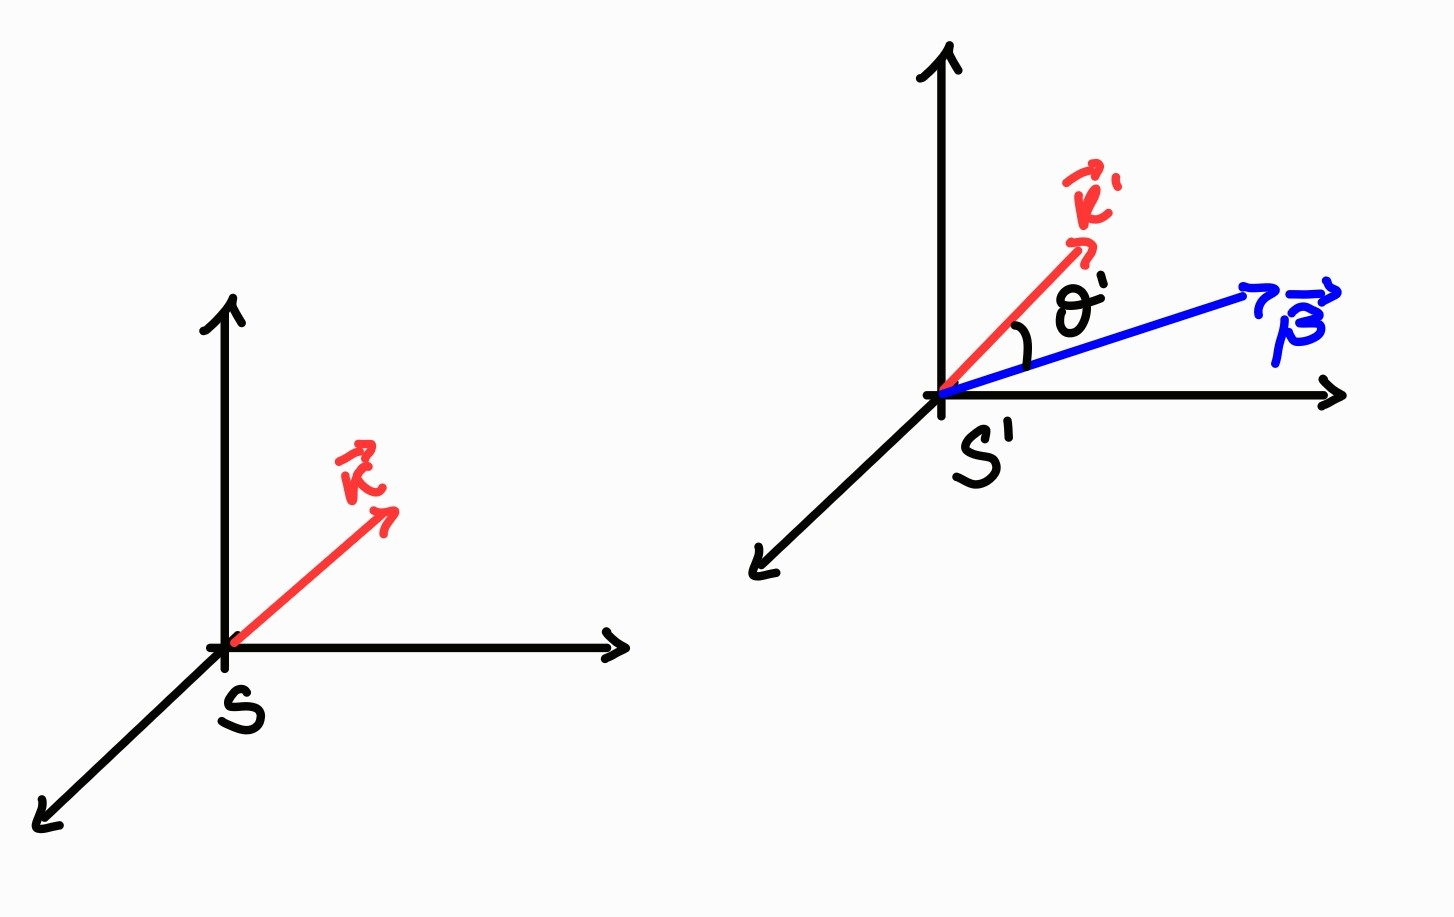
\includegraphics[width=0.40\textwidth]{Immagini/Doppler.jpg}
    \caption{ Sistemi di riferimento inerziali con vettore d'onda}
    \label{fig:Doppler}
\end{figure}

La trasformazione di Lorentz che lega le due quantità è:
\begin{equation}
\begin{gathered}
      k^{\alpha}\xrightarrow[\text{}]{\text{L}}k'^{\beta}=\Lambda\indices{^\beta_\nu}(\Vec{v}) k^{\nu}\\
         k'^{\alpha}\xrightarrow[\text{}]{\text{L}}k^{\beta}=\Lambda\indices{^\beta_\nu}(-\Vec{v}) k'^{\nu}
\end{gathered}
\end{equation}
in particolare sviluppiamo la componente temporale:
\begin{equation}
   \begin{split}
       k^0=\Lambda\indices{^0_\beta} k'^{\beta}=\Lambda\indices{^0_0} k'^{0}+\Lambda\indices{^0_i} k'^{i}=\gamma k'^{0}+\beta_i\gamma k'^{i}&=\gamma[ k'^{0}+\beta_i k'^{i}]=\gamma[ k'^{0}+\Vec{\beta}\Vec{k}']\\
       &=\gamma[ k'^{0}+|\Vec{\beta}||\Vec{k}'|\cos{\theta'}]=\gamma k'^{0}[ 1+|\Vec{\beta}|\cos{\theta'}]
   \end{split}
\end{equation}
ricordando $k^0=|\Vec{k}|=\dfrac{\omega}{c}$ e definendo la frequenza come $\nu=\dfrac{\omega}{2\pi}$ otteniamo:
\begin{equation}\phantomsection\label{eq:Doppler_fre}
       \dfrac{\omega}{c}=\gamma\dfrac{\omega'}{c}[ 1+|\Vec{\beta}|\cos{\theta'}] \implies  \nu=\gamma\nu'[ 1+|\Vec{\beta}|\cos{\theta'}]=\nu'\dfrac{1+|\Vec{\beta}|\cos{\theta'}}{\sqrt{1-\beta^2}}
\end{equation}

Studiamo, ora, il caso particolare nel quale $\Vec{\beta}\parallel\Vec{x}$ e consideriamo l'onda elettromagnetica la cui direzione di moto forma l'angolo $\theta$ con l'asse $x$ e forma l'angolo $\theta'$ con l'asse $x'$.
\begin{figure}[h]
    \centering
    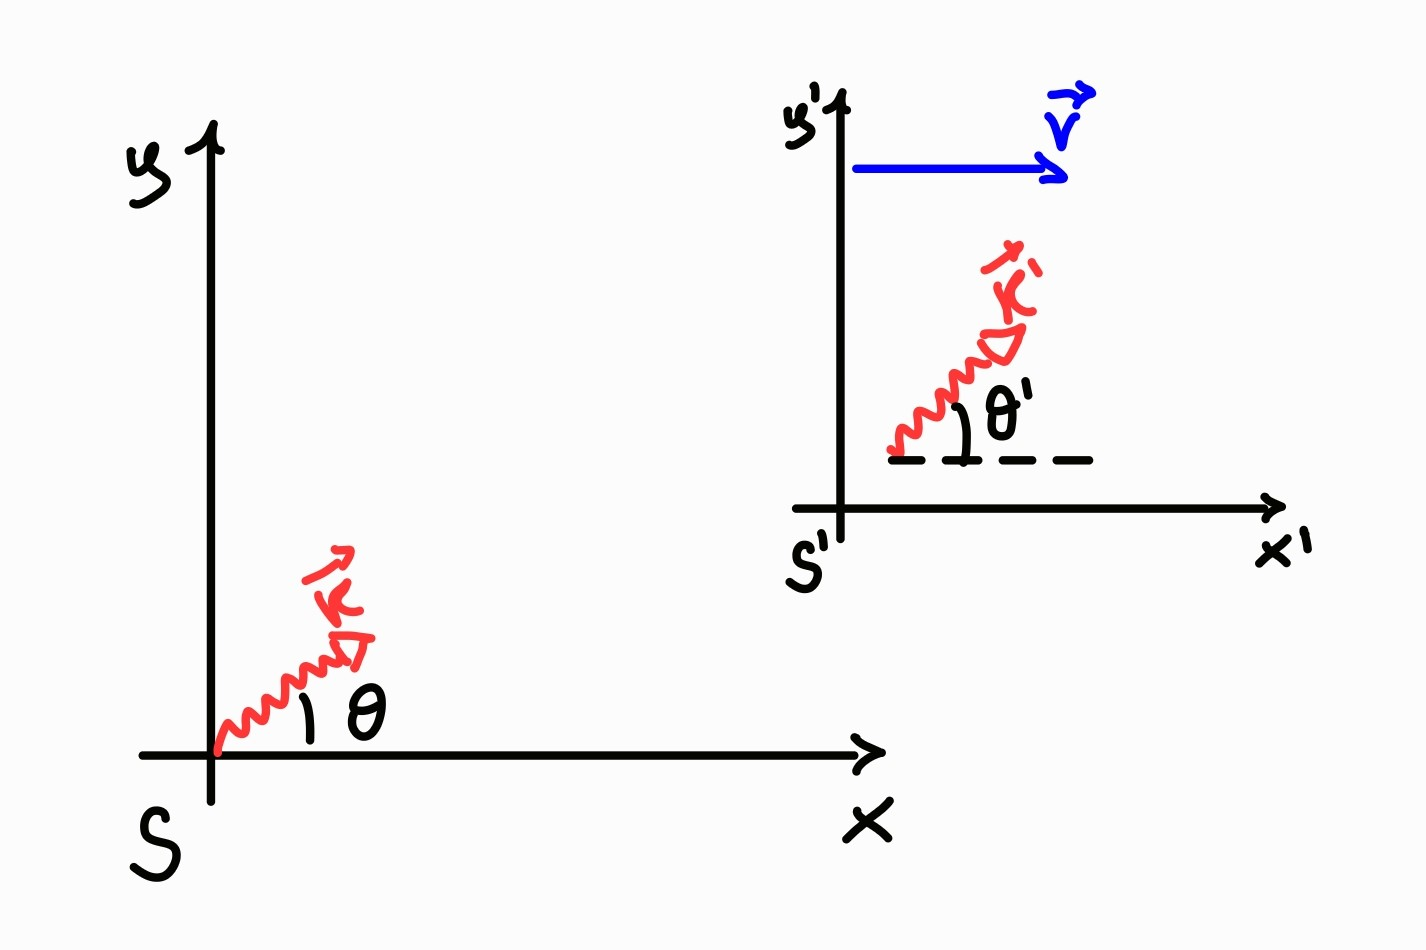
\includegraphics[width=0.40\textwidth]{Immagini/Doppler_unidirezionale .jpg}
    \caption{ Sistemi di riferimento inerziali di moto relativo lungo x e con onda elettromagnetica in direzione arbitraria }
    \label{fig:Doppler_x}
\end{figure}

Invertendo la \eqref{eq:Doppler_fre}, otteniamo:
\begin{equation}
        \nu'=\nu\dfrac{\sqrt{1-\beta^2}}{1+|\Vec{\beta}|\cos{\theta'}}
\end{equation}
studiamo le componenti spaziali x e y del vettore d'onda:
\begin{equation}
   \begin{gathered}
       k^1=\Lambda\indices{^1_\beta} k'^{\beta}=\Lambda\indices{^1_0} k'^{0}+\Lambda\indices{^1_i} k'^{i}=\gamma\beta k'^{0}+\gamma k'^{1}\\
       \implies|\Vec{k}|\cos{\theta}=\gamma k'^{0}[ \beta+\cos{\theta'}]
   \end{gathered}
\end{equation}
esplicito le frequenze sostituendo come prima 
\begin{equation}
     \nu\cos{\theta}=\nu'\dfrac{\beta+\cos{\theta'}}{\sqrt{1-\beta^2}}
\end{equation}
la componete y sarà:
\begin{equation}
   \begin{gathered}
       k^2=\Lambda\indices{^2_\beta} k'^{\beta}=\Lambda\indices{^2_0} k'^{0}+\Lambda\indices{^2_i} k'^{i}= k'^{2}\\
       \implies|\Vec{k}|\sin{\theta}=|\Vec{k}'|\sin{\theta'}\implies \nu\sin{\theta}=\nu'\sin{\theta'}
   \end{gathered}
\end{equation}
concludiamo che si modifica la componente longitudinale al moto, ma non quella trasversale. Determiniamo la relazione che lega i due angoli:
\begin{equation}
     \tan{\theta}=\dfrac{\sin{\theta'}\sqrt{1-\beta^2}}{\cos{\theta'}+\beta}
\end{equation}
Concludiamo questa parte studiando due casi notevoli. Chiamiamo \textit{effetto doppler longitudinale} il caso in cui $\theta'=\theta=0$
\begin{equation}
    \nu=\nu'\dfrac{1+|\Vec{\beta}|\cos{\theta'}}{\sqrt{1-\beta^2}}=\nu'\dfrac{\sqrt{1+\beta}}{\sqrt{1-\beta}}
\end{equation}
 invece, chiamiamo \textit{effetto doppler trasverso} il caso in cui $\theta'=\dfrac{\pi}{2}$
\begin{equation}
    \nu=\nu'\dfrac{1+|\Vec{\beta}|\cos{\theta'}}{\sqrt{1-\beta^2}}=\nu'\dfrac{1}{\sqrt{1-\beta^2}}
\end{equation}
possiamo notare che il primo termine correttivo nell'effetto doppler trasverso è del secondo ordine in $\beta$, questo significa che sperimentalmente risulta più difficile, rispetto all'effetto doppler longitudinale, da misurare.

\subsection{Soluzione con sorgenti}
Consideriamo le equazioni di Maxwell con la condizione di gauge di Lorentz \eqref{eq:Max_gauge} nel caso generale in cui siano presenti sorgenti:
\begin{equation}
\begin{cases}\phantomsection\label{eq:Maxwell_sorgenti}
  \Box A^\nu(t,\Vec{x})=\dfrac{4\pi}{c}j^\nu(t,\Vec{x})\\
  \partial_\mu A^\mu=0
\end{cases}
\end{equation}
la soluzione sarà data dalla somma di una parte omogenea, già discussa in sezione \ref{sec:2.7}, e di una parte particolare. Il metodo che utilizzeremo è detto delle funzioni di Green.

Introduciamo una \textit{funzione di Green} come una funzione biscalare\footnote{Ossia uno scalare che dipende da due eventi.} $D(t,\Vec{x};t',\Vec{x}')$ che soddisfa la relazione:
\begin{equation}\phantomsection\label{eq:Def_Green}
    \Box_x D(t,\Vec{x};t',\Vec{x}')=\delta^4(x-x')=\delta(ct-ct')\delta^3(\Vec{x}-\Vec{x}')
\end{equation}
specifichiamo che il pedice all'operatore dalembertiano indica che quest'ultimo agisce sulle coordinate non primate. Dimostriamo rapidamente che l'oggetto appena introdotto è uno scalare.
\begin{proof}
    Dalla proprietà della delta sappiamo
    \begin{equation}
        \int d^4xf(x)\delta^4(x-y)=f(y)
    \end{equation}
    in particolare se poniamo $f(x)=1$
     \begin{equation}
        \int d^4x\delta^4(x)=1
    \end{equation}
    concludiamo che essendo la misura uno scalare e il risultato dell'integrazione anche, ne consegue necessariamente che la $\delta^4(x)$ sarà uno scalare e, dalla definizione, lo sarà anche $D(t,\Vec{x};t',\Vec{x}')$.
    \end{proof}
Poiché lo spazio di Minkowski è omogeneo, la funzione di Green deve essere invariante per traslazioni, quindi la sua dipendenza non sarà definita dai due eventi separatamente, bensì dalla loro differenza. Pertanto possiamo riscrivere la dipendenza come:
\begin{equation}
   D(t-t',\Vec{x}-\Vec{x}')=D(x-x')
\end{equation}
quindi possiamo riscrivere anche la definizione della funzione di Green, come:
\begin{equation}
    \Box_x D(x-x')=\delta^4(x-x')
\end{equation}
Si può dimostrare, e lo faremo subito, che una soluzione particolare della \eqref{eq:Maxwell_sorgenti} è:

\begin{equation}\phantomsection\label{eq:Maxwell_sorgenti_sol}
  A^\alpha(t,\Vec{x})=\dfrac{4\pi}{c}\int d^4x'D(x-x')j^\alpha(t',\Vec{x}')\footnote{Possiamo notare che in questa forma il potenziale ha l'aspetto di un prodotto di convoluzione: \\$(f*g)(x)=\int_{\mathbb{R}^n}f(x-y)g(y)dy$.}
\end{equation}
applicando l'operatore di D'Alembert, otteniamo:\begin{equation}
  \Box_x A^\alpha(t,\Vec{x})=\dfrac{4\pi}{c}\int d^4x'\Box_xD(x-x')j^\alpha(t',\Vec{x}')=\dfrac{4\pi}{c}\int d^4x'\delta^4(x-x')j^\alpha(t',\Vec{x}')=\dfrac{4\pi}{c}j^\alpha(t,\Vec{x})
\end{equation}
la delta di Dirac ha supporto solo quando i due eventi coincidono, quindi l'integrale si riduce all'equazione iniziale. Concludiamo che conoscendo una funzione di Green, in linea di principio, grazie alla \eqref{eq:Maxwell_sorgenti_sol}, abbiamo una soluzione. A questo punto dobbiamo determinare una forma analitica per la funzione di Green, per farlo procederemo utilizzando la trasformata di Fourier\footnote{ Difatti, spesso, per risolvere equazioni differenziali si fa uso delle trasformate di Fourier, questo perché un'equazione differenziale, nello spazio iniziale, diventa una semplice equazione algebrica, nello spazio di Fourier.}.

Rappresentiamo, quindi, la funzione di Green con una trasformata di Fourier quadridimensionale:
\begin{equation}\phantomsection\label{eq:Green_Fourier}
  D(x-x')=\dfrac{1}{(2\pi)^4}\int d^4k\quad e^{-ik_\alpha(x^\alpha-x'^\alpha)} \Tilde{D}(k)
\end{equation}
mentre la rappresentazione della delta di Dirac è:
\begin{equation}\phantomsection\label{eq:Dirac_Fourier}
  \delta^4(x-x')=\dfrac{1}{(2\pi)^4}\int d^4k\quad e^{-ik_\alpha(x^\alpha-x'^\alpha)} 
\end{equation}
Dunque la definizione della funzione di Green \eqref{eq:Def_Green} diventa, in termini delle rappresentazioni di Fourier:
\begin{equation}
\begin{gathered}
        \Box_x D(x-x')=\delta^4(x-x')\\  \Box_x \dfrac{1}{(2\pi)^4}\int d^4k\quad e^{-ik_\alpha(x^\alpha-x'^\alpha)} \Tilde{D}(k)=\dfrac{1}{(2\pi)^4}\int d^4k\quad e^{-ik_\alpha(x^\alpha-x'^\alpha)} \\
        \dfrac{1}{(2\pi)^4}\int d^4k\quad (-k_\mu k^\mu)e^{-ik_\alpha(x^\alpha-x'^\alpha)} \Tilde{D}(k)=\dfrac{1}{(2\pi)^4}\int d^4k\quad e^{-ik_\alpha(x^\alpha-x'^\alpha)}
\end{gathered}
\end{equation}
ove ricordiamo che $\Box_x=\partial_\mu\partial^\mu$ e l'unico termine che dipende da $x$ è l'esponenziale. Inoltre, per la completezza delle funzioni nello spazio di Fourier possiamo scrivere:\begin{equation}
-k_\mu k^\mu \Tilde{D}(k)=1 \implies \Tilde{D}(k)=-\dfrac{1}{k_\mu k^\mu}=-\dfrac{1}{(k_0)^2 -|\Vec{k}|^2}
\end{equation}
ottenendo, così, un equazione algebrica. Per semplificare la notazione consideriamo $|\Vec{k}|^2=k^2$. 

Sostituendo quanto appena ottenuto nella \eqref{eq:Green_Fourier}:
\begin{equation}\phantomsection\label{eq:int_green}
\begin{split}
     D(x-x')&=\dfrac{1}{(2\pi)^4}\int d^4k\quad e^{-ik_\alpha(x^\alpha-x'^\alpha)}\dfrac{1}{k^2-k\indices{_0^2}}\\
     &=\dfrac{1}{(2\pi)^4}\int d^3k\quad e^{i\Vec{k}(\Vec{x}-\Vec{x}')}\int^{\infty}_{-\infty} dk_0\quad e^{-ik_0(ct-ct')}\dfrac{1}{k^2-k\indices{_0^2}}
\end{split}
\end{equation}

si pone il problema di scegliere una funzione di Green tra le infinite possibili.
Per ragioni fisiche di causalità richiediamo che la funzione di Green soddisfi la \textit{condizione di ritardo}, ossia:
\begin{equation}
    D(x-x')=0 \qquad \forall t<t'
\end{equation}
fisicamente tale condizione significa che la funzione di Green non dipende da eventi che siano temporalmente successivi a quello dell'osservatore. 

Ora, dobbiamo risolvere l'integrale \eqref{eq:int_green}, notiamo che presenta due poli sul percorso di integrazione. 
\begin{equation}
    k^2-k\indices{_0^2}=(k+k_0)(k-k_0)
\end{equation}
Per risolverlo pensiamo, momentaneamente, a $k_0$ come complesso e facciamo la prescrizione che consiste nella sottrazione di una parte immaginaria tendente a zero, cosicché il percorso sia integrabile.
\begin{equation}
    k^2-k\indices{_0^2}=(k+k_0)(k-k_0)=\lim_{\epsilon\to0^+} (k+i\epsilon+k_0)(k-i\epsilon-k_0)
\end{equation}
\begin{figure}[H]
    \centering
    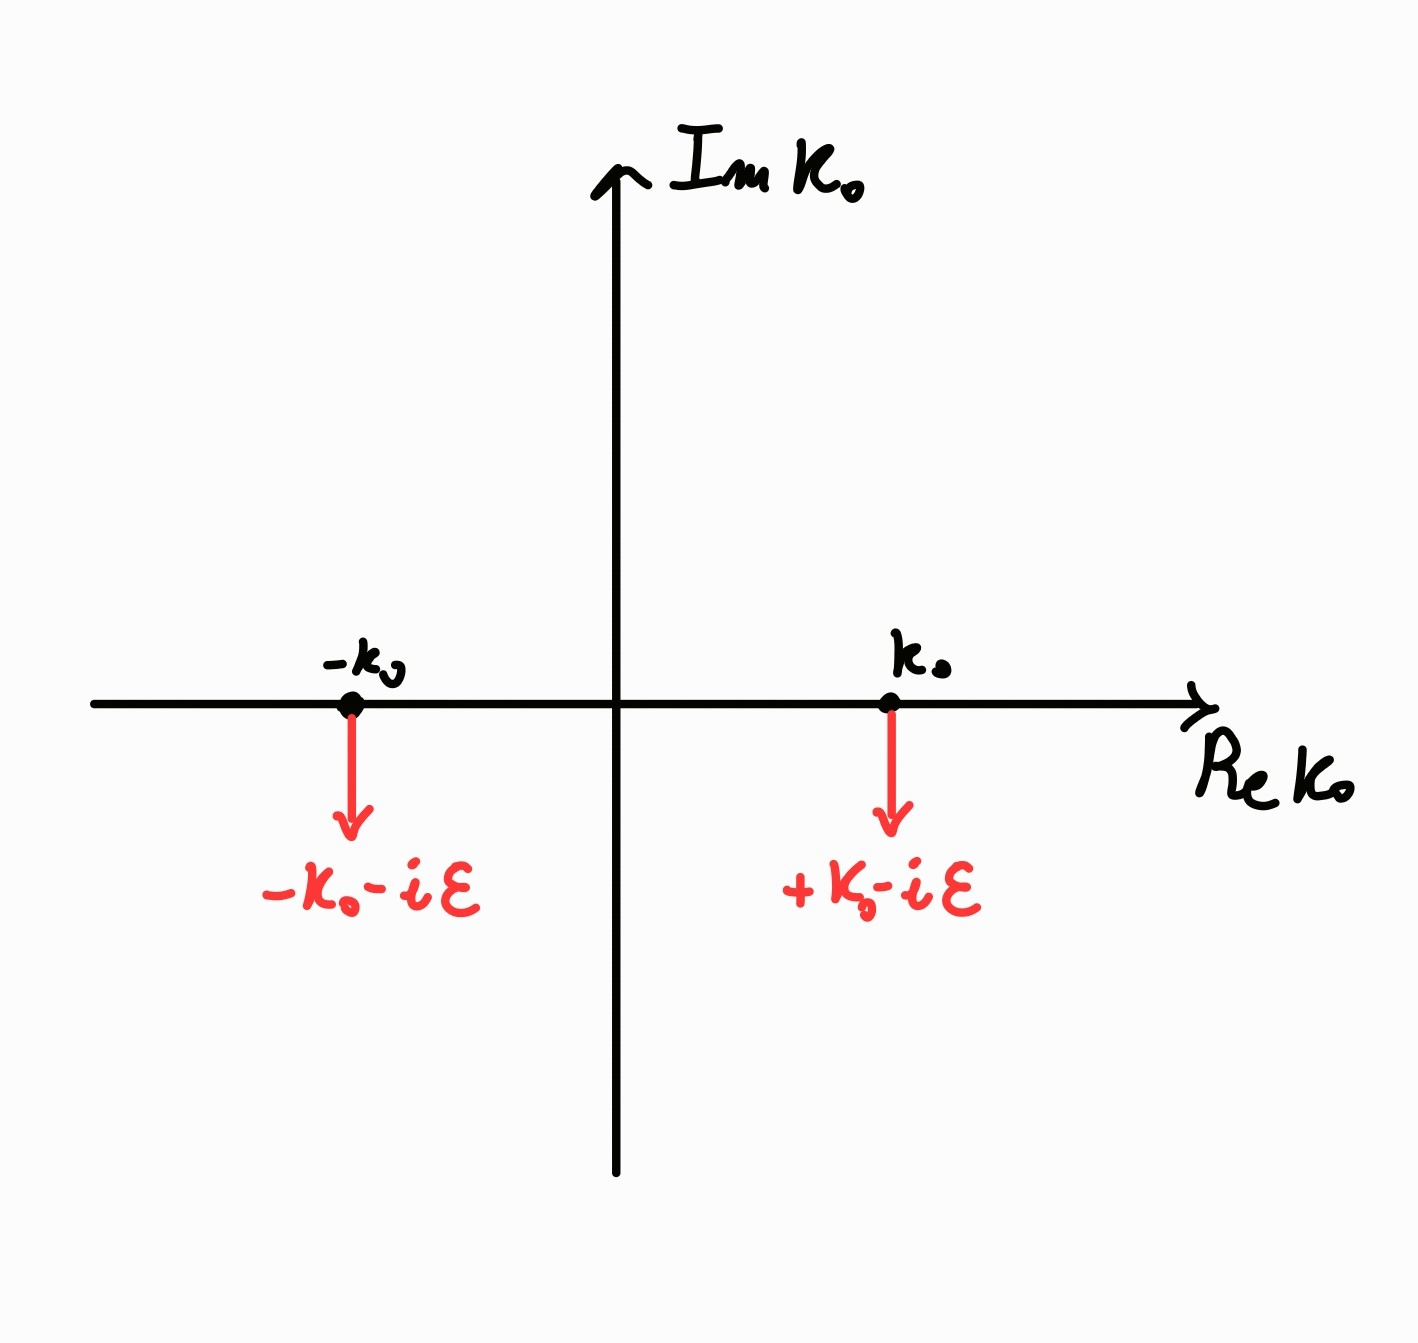
\includegraphics[width=0.40\textwidth]{Immagini/Prescrizione.jpg}
    \caption{Spostamento dei punti singolari al di sotto della retta reale di integrazione.}
    \label{fig:prescrizione}
\end{figure}

Definiamo l'integrale sul piano complesso di $k_0$
\begin{equation}\phantomsection\label{eq:int_compl}
J_{ret}(k)=\lim_{\epsilon\to0^+} \int^{\infty}_{-\infty} dk_0\quad \dfrac{e^{-ick_0(t-t')}}{(k+i\epsilon+k_0)(k-i\epsilon-k_0)}
\end{equation}
\begin{figure}[H]
    \centering
    \subfloat[\centering Integrazione semipiano superiore.]{{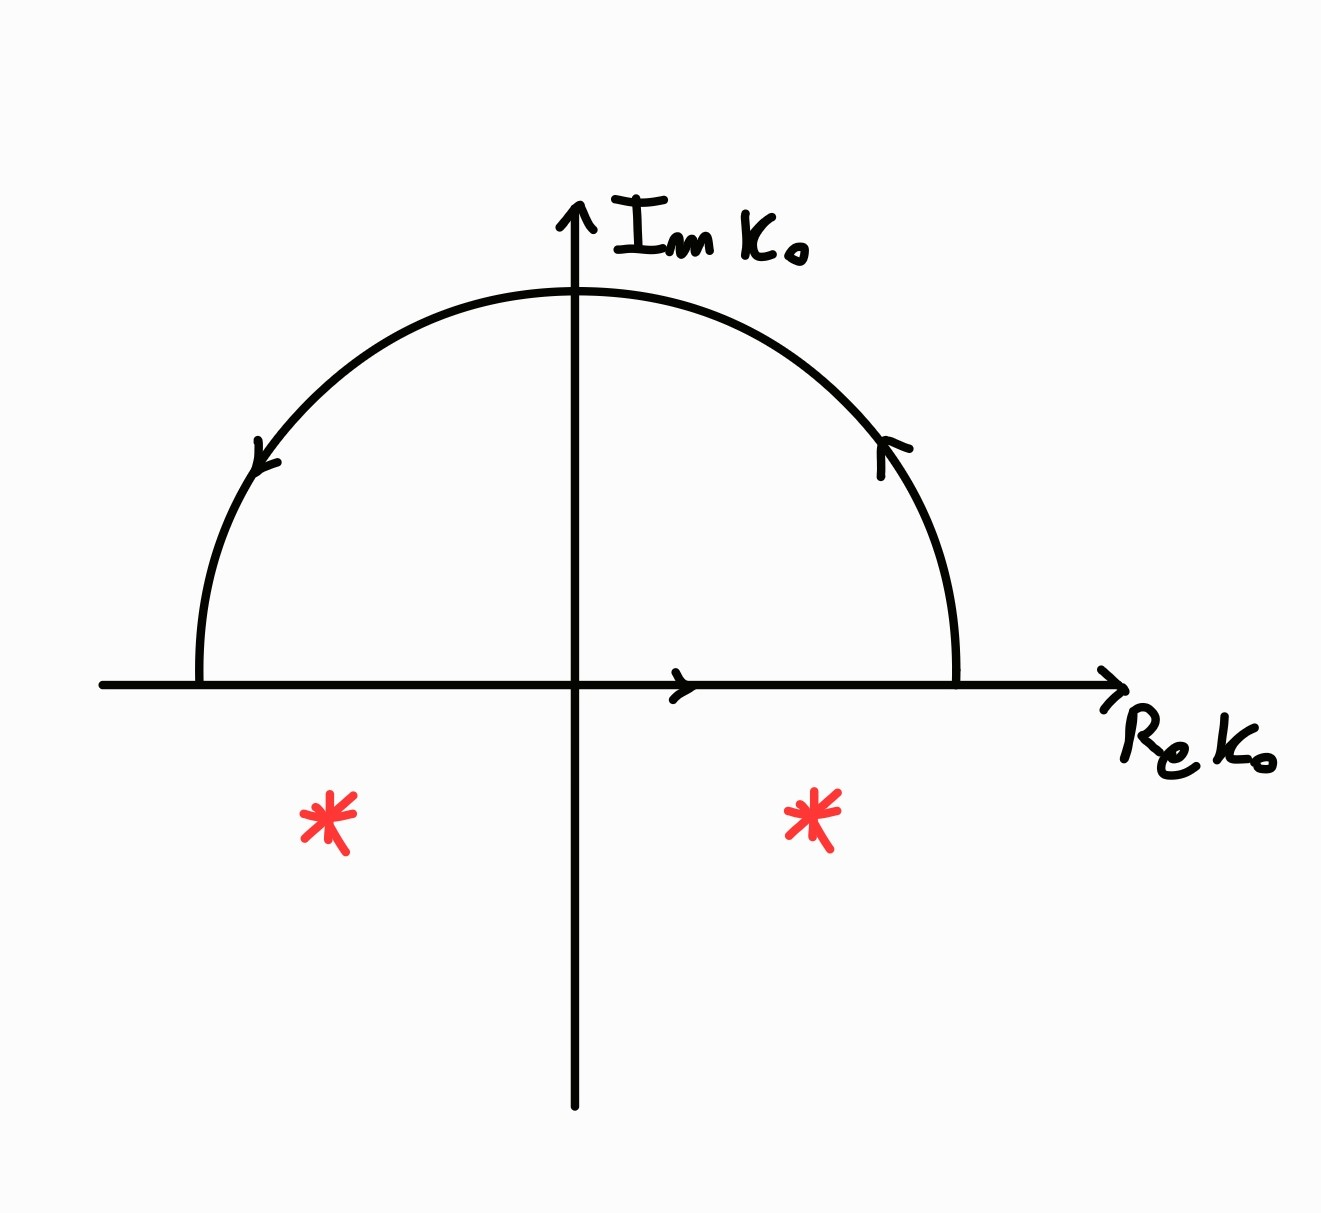
\includegraphics[width=5cm]{Immagini/Residuo_sup.jpg} }}%
    \qquad
    \subfloat[\centering Integrazione semipiano inferiore.]{{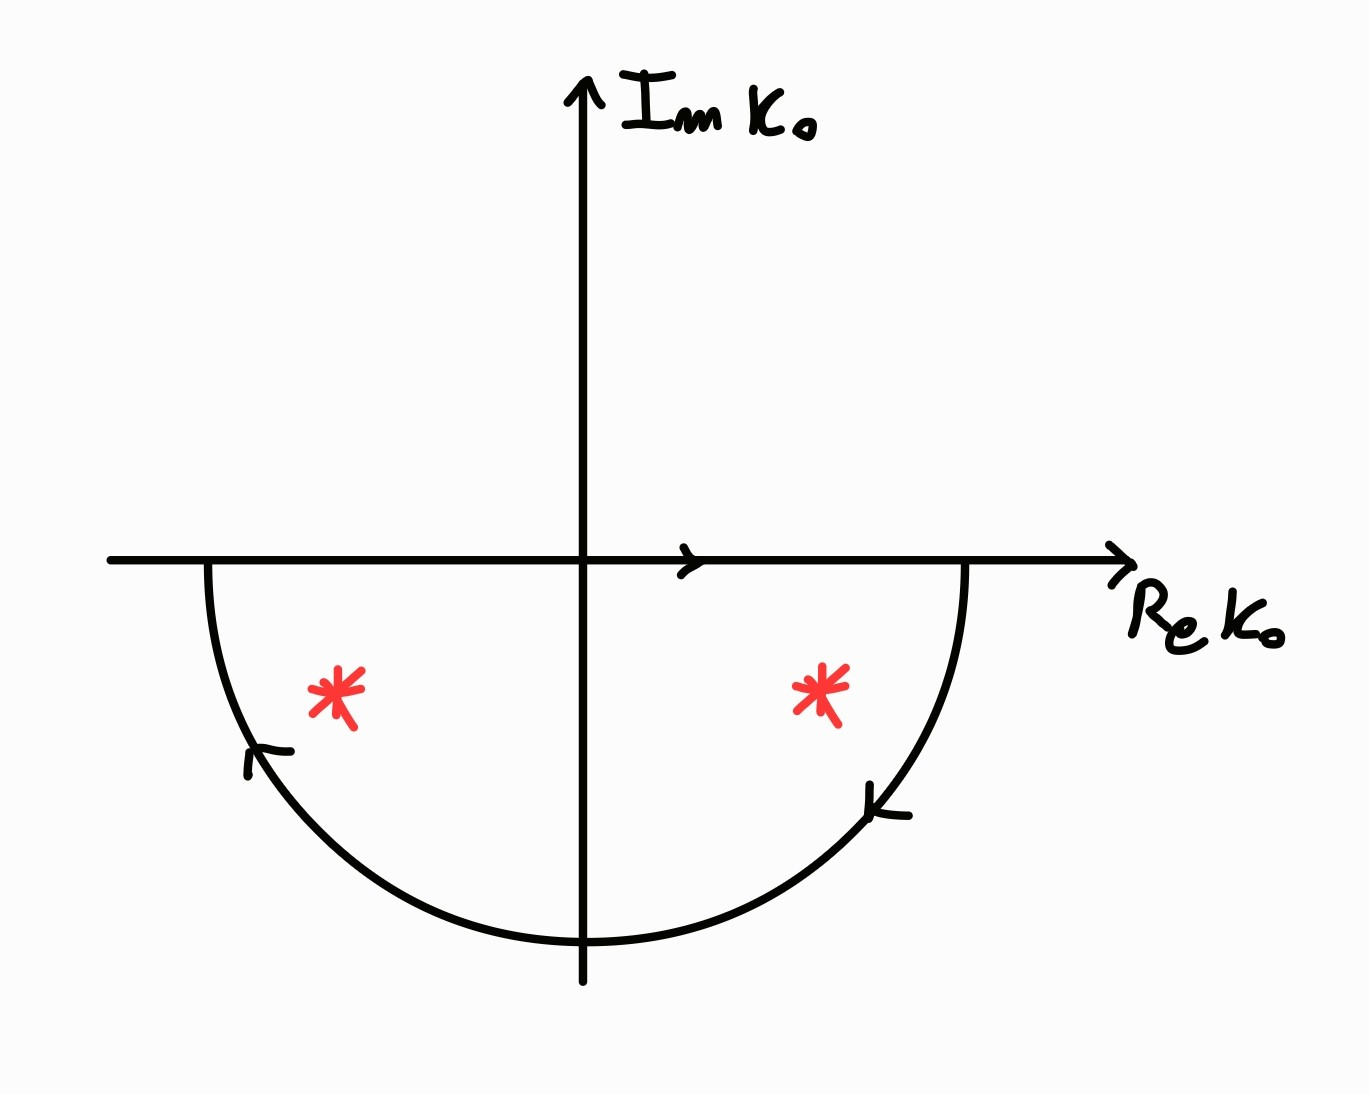
\includegraphics[width=5cm]{Immagini/Residuo_inf.jpg} }}%
    \caption{Integrazione nel piano complesso.}%
    \label{fig:Residuo}%
\end{figure}
Per risolvere l'integrale \eqref{eq:int_compl} consideriamo i percorsi rappresentati in Fig.\ref{fig:Residuo}. In particolare, per $t<t'$ abbiamo che la funzione integranda è analitica nel semipiano superiore, quindi, per il lemma di Jordan, il risultato dell'integrazione è nullo.
Mentre per $t>t'$ la funzione è sempre analitica ed applicando il teorema dei residui, avendo due poli semplici, otteniamo:
 \begin{equation}
J_{ret}(k)=-2\pi i \dfrac{e^{ick(t-t')}-e^{-ick(t-t')}}{2k}\Theta(ct-ct')
\end{equation}
ove la funzione $\Theta(ct-ct')$ non è altro che una funzione a gradino che vale $0$ per $t<t'$ e $1$ per $t>t'$\footnote{Questa ci serve unicamente per ricordarci della condizione di ritardo.}.
Possiamo manipolare il risultato ottenuto
 \begin{equation}
 \begin{aligned}
      J_{ret}(k)&=-2\pi i \dfrac{e^{ick(t-t')}-e^{-ick(t-t')}}{2k}\Theta(ct-ct')=  2\pi\dfrac{e^{ick(t-t')}-e^{-ick(t-t')}}{2ki}\Theta(ct-ct')\\
      &=2\pi\dfrac{\sin{[ck(t-t')]}}{k}\Theta(ct-ct')
 \end{aligned}
\end{equation}
Sostituendolo nella \eqref{eq:int_green} otteniamo la Funzione di Green ritardata:
\begin{equation}
   \begin{aligned}
        D_{ret}(x-x')&=\dfrac{1}{(2\pi)^4}\int d^3k\quad e^{i\Vec{k}(\Vec{x}-\Vec{x}')}2\pi\dfrac{\sin{[ck(t-t')]}}{k}\Theta(ct-ct')\\
     &=\dfrac{1}{(2\pi)^3}\int d^3k\quad e^{i\Vec{k}(\Vec{x}-\Vec{x}')}\dfrac{\sin{[ck(t-t')]}}{k}\Theta(ct-ct')
   \end{aligned}
\end{equation}
Ci rimane solamente da risolvere l'integrale, per farlo definiamo $\Vec{R}=\Vec{x}-\Vec{x}'$ ed in particolare scegliamo\footnote{Possiamo farlo perché, nello spazio di Minkowki, abbiamo l'invarianza per rotazioni.} $\Vec{x}-\Vec{x}'\parallel \Vec{z}$. Inoltre consideriamo il prodotto $\Vec{k}(\Vec{x}-\Vec{x}')=kR\cos{\theta}$, ove $\theta$, per la scelta di prima, è l'angolo azimutale. A questo punto passiamo in coordinate sferiche\footnote{Ricordiamo che la misura cambia in $d^3k=k^2dk\sin{\theta}d\theta d\phi$.} e riscriviamo l'integrale.
\begin{equation}\phantomsection\label{eq:ret_green}
   \begin{aligned}
        D_{ret}(x-x')&=\dfrac{1}{(2\pi)^3}\int k^2dk\sin{\theta}d\theta d\phi \quad e^{ikR\cos{\theta}}\dfrac{\sin{[ck(t-t')]}}{k}\Theta(ct-ct')\\
        &=\dfrac{1}{(2\pi)^3}\int_0^\infty kdk\sin{[ck(t-t')]}\int_0^\pi d\theta \sin{\theta}e^{ikR\cos{\theta}} \int_0^{2\pi}d\phi \quad\Theta(ct-ct')\\
        &=\dfrac{1}{(2\pi)^2}\int_0^\infty kdk\sin{[ck(t-t')]}\int_0^\pi d\theta \sin{\theta}e^{ikR\cos{\theta}}  \quad\Theta(ct-ct')
   \end{aligned}
\end{equation}
Consideriamo il cambio di variabile $\xi=\cos{\theta}$, da cui $d\theta=-\dfrac{d\xi}{\sin{\theta}}$
\begin{equation}
   \begin{aligned}
        D_{ret}(x-x')&=\dfrac{1}{(2\pi)^2}\int_0^\infty kdk\sin{[ck(t-t')]}\int_0^\pi d\theta \sin{\theta}e^{ikR\cos{\theta}}  \quad\Theta(ct-ct')\\
        &=\dfrac{1}{(2\pi)^2}\int_0^\infty kdk\sin{[ck(t-t')]}\int_{-1}^1 d\xi e^{ikR\xi}  \quad\Theta(ct-ct')\\
        &=\dfrac{1}{(2\pi)^2}\int_0^\infty kdk\sin{[ck(t-t')]} \dfrac{e^{ikR}-e^{-ikR}}{ikR}  \quad\Theta(ct-ct')\\
         &=\dfrac{1}{(2\pi)^2}\int_0^\infty dk\sin{[ck(t-t')]} \dfrac{e^{ikR}-e^{-ikR}}{iR} \dfrac{2}{2} \quad\Theta(ct-ct')\\
          &=\dfrac{2}{(2\pi)^2R}\int_0^\infty dk\sin{[ck(t-t')]} \sin{kR}  \quad\Theta(ct-ct')\\
   \end{aligned}
\end{equation}
la funzione integranda, così ottenuta, è ovviamente pari poiché prodotto di funzioni dispari
\begin{equation}
   \begin{aligned}
        D_{ret}(x-x')&=\dfrac{1}{(2\pi)^2R}\int_{-\infty}^\infty dk\sin{[ck(t-t')]} \sin{kR}  \quad\Theta(ct-ct')\\
        &=\dfrac{1}{(2\pi)^2R}\left(-\dfrac{1}{4}\right)\int_{-\infty}^\infty dk [e^{ick(t-t')}-e^{-ick(t-t')}][e^{ikR}-e^{-ikR}]  \quad\Theta(ct-ct')\\
        &=\dfrac{1}{4(2\pi)^2R}\int_{-\infty}^\infty dk [e^{-ick(t-t')}-e^{ick(t-t')}][e^{ikR}-e^{-ikR}]  \quad\Theta(ct-ct')\\
         &=\dfrac{1}{4(2\pi)^2R}\int_{-\infty}^\infty dk \{e^{-ik[c(t-t')-R]}-e^{-ik[c(t-t')+R]}\\&\qquad \qquad\qquad\qquad\quad-e^{ik[c(t-t')+R]}+e^{ik[c(t-t')-R]} \}\Theta(ct-ct')\\
   \end{aligned}
\end{equation}
Ora, ricordando la \eqref{eq:Dirac_Fourier}, per una sola dimensione, e ricordando la proprietà $\delta(x)=\delta(-x)$
\begin{equation}
   \begin{aligned}
        D_{ret}(x-x')=\dfrac{2\pi}{4(2\pi)^2R}&\{ \delta[c(t-t')-R]-\delta[c(t-t')+R]\\
       & -\delta[c(t-t')+R]+\delta[c(t-t')-R] \}\Theta(ct-ct')\\
   \end{aligned}
\end{equation}
quello che sappiamo è che la delta ha supporto solo quando il suo argomento è nullo. Analizziamo gli argomenti: la sottrazione $t-t'$ è positiva sotto la garanzia della funzione $\Theta(ct-ct')$ e $R=|\Vec{x}-\Vec{x}'|$ è positiva per definizione. Quindi gli argomenti delle delta nelle quali i fattori sono sommati non si annulleranno mai, dunque, ha senso tenere solo $\delta[c(t-t')-R]$:
\begin{equation}\phantomsection\label{eq:Green_ret}
        D_{ret}(x-x')=\dfrac{2}{4(2\pi)R}\delta[c(t-t')-R]\Theta(ct-ct')=\dfrac{1}{4\pi}\dfrac{\delta[c(t-t')-R]}{|\Vec{x}-\Vec{x}'|}\Theta(ct-ct')
\end{equation}
questa è la funzione di Green ritardata per l'operatore di D'Alembert.

Sostituendola nella \eqref{eq:Maxwell_sorgenti_sol}
\begin{equation}
  A_{ret}^\alpha(t,\Vec{x})=\dfrac{4\pi}{c}\int d^4x'D(x-x')j^\alpha(t',\Vec{x}')=\dfrac{1}{c}\int d(ct')d^3x'\dfrac{\delta[c(t-t')-|\Vec{x}-\Vec{x}'|]}{|\Vec{x}-\Vec{x}'|}j^\alpha(t',\Vec{x}')
\end{equation}
ci rimane da calcolare questo integrale. L'integrazione in $t'$ è immediata, poiché la delta avrà supporto solo per 
\begin{equation}\phantomsection\label{eq:t_ret}
    c(t-t')=|\Vec{x}-\Vec{x}'| \implies t'=t-\dfrac{|\Vec{x}-\Vec{x}'|}{c}
\end{equation}
quindi l'unico contributo dell'integrazione sarà dato da $t'$:
\begin{equation}\phantomsection\label{eq:soluz_rita}
  A_{ret}^\alpha(t,\Vec{x})=\int d^3x'\dfrac{j^\alpha(t-\dfrac{R}{c},\Vec{x}')]}{|\Vec{x}-\Vec{x}'|}
\end{equation}
\`E doveroso fare alcune osservazioni. Se consideriamo (come mostrato in Fig.\ref{fig:Green}) un osservatore all'evento $P(t,\Vec{x})$ e una carica all'evento $Q=(t',\Vec{x}')$, la relazione \eqref{eq:soluz_rita} descrive il campo percepito dall'osservatore. Il fatto che tale relazione dipenda dalla definizione \eqref{eq:t_ret} del tempo ritardato mostra la causalità intrinseca alla soluzione trovata. Questo significa che ciò che l'osservatore \say{vede} è ristretto a ciò che è contenuto nel suo cono di luce passato\footnote{Viene escluso il cono di luce futuro dalla condizione di ritardo.}, questo perché la radiazione elettromagnetica ha velocità finita.
\begin{figure}[H]
    \centering
    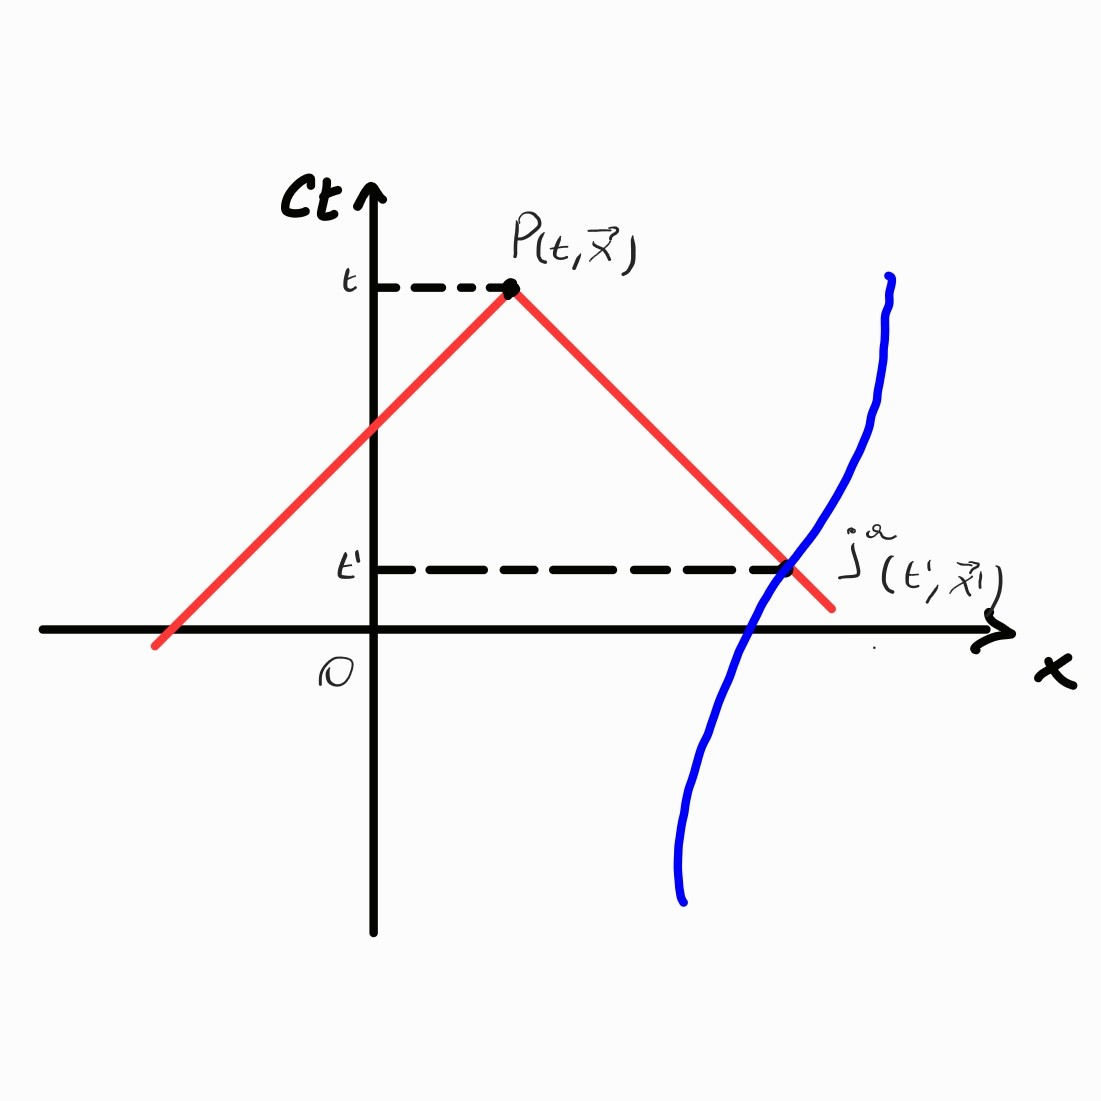
\includegraphics[width=0.35\textwidth]{Immagini/Green.jpg}
    \caption{La rappresentazione grafica di $c=\dfrac{|\Vec{x}-\Vec{x}'|}{t-t'}$ non è altro che il cono di luce.}
    \label{fig:Green}
\end{figure}
Nelle teorie classiche non è così, le velocità sono considerate infinite. Per la teoria gravitazionale di Newton abbiamo che il campo gravitazionale varia istantaneamente secondo l'equazione di Poisson $\nabla^2\phi=4\pi\sigma\rho$.
 
 Ci rimane da mostrare che la funzione di Green sia Lorentz invariante e che soddisfi la condizione di gauge di Lorentz. Per verificare l'invarianza consideriamo gli eventi $x^\alpha=(x^0,\Vec{x})$ e $x'^\alpha=(x'^0,\Vec{x}')$ e definiamo la delta Dirac che sappiamo essere invariante:
 \begin{equation}
 \begin{aligned}
      \delta[(x^\alpha-x'^\alpha)(x_\alpha-x'_\alpha)]&= \delta[(x_0-x'_0)^2-|\Vec{x}-\Vec{x}'|^2]= \delta[(x_0-x'_0)^2-R^2]\\
      &=\delta\{[(x_0-x'_0)+R][(x_0-x'_0)-R]\}
 \end{aligned}
 \end{equation}
 ricordiamo la proprietà $\delta(g(x))=\sum_i \dfrac{\delta(x-x_i)}{|\frac{dg}{dx}|_{x_i}}$ ove $g$ è una funzione tale per cui $g(x_i)=0$, otteniamo:
 \begin{equation}
     \delta[(x^\alpha-x'^\alpha)(x_\alpha-x'_\alpha)]= \dfrac{1}{2R}[\delta(x^0-x'^0+R)+\delta(x^0-x'^0-R)]
 \end{equation}
 se moltiplichiamo la condizione di ritardo possiamo omettere la delta $\delta(x^0-x'^0+R)$ poiché l'argomento non si annulla mai e quindi non ha supporto
  \begin{equation}
  \begin{aligned}
     \delta[(x^\alpha-x'^\alpha)(x_\alpha-x'_\alpha)]\Theta(ct-ct')&= \dfrac{1}{2R}[\delta(x^0-x'^0+R)+\delta(x^0-x'^0-R)]\Theta(ct-ct')\\
     &=\dfrac{1}{2R}[\delta(x^0-x'^0-R)]\Theta(ct-ct')\\
     &\implies \delta(x^0-x'^0-R)=(2R)\delta[(x^\alpha-x'^\alpha)(x_\alpha-x'_\alpha)]
  \end{aligned}
 \end{equation}
 sostituendo nella \eqref{eq:Green_ret} otteniamo:
 \begin{equation}\phantomsection\label{eq:Green_inva}
        D_{ret}(x-x')=\dfrac{1}{4\pi}\dfrac{\delta[c(t-t')-R]}{R}\Theta(ct-ct')=\dfrac{1}{2\pi}\delta[(x^\alpha-x'^\alpha)(x_\alpha-x'_\alpha)]\Theta(ct-ct')
\end{equation}
in questa forma si vede chiaramente che la funzione di Green è uno scalare ed ogni sua parte è Lorentz invariante. Inoltre, la funzione di Green ha supporto solo quando $x\alpha=x'\alpha$ ossia se $x\alpha-x'\alpha$ è un vettore di tipo luce, geometricamente significa che la funzione di Green ha supporto solo sul cono di luce.

Ora dimostriamo che la soluzione trovata \eqref{eq:soluz_rita} soddisfi il gauge di Lorentz, altrimenti il lavoro è sarebbe stato vano.\begin{equation}
  \partial_\alpha A_{ret}^\alpha(t,\Vec{x})=\dfrac{4\pi}{c}\int d^4x'\partial_\alpha D_{ret}(x-x')j^\alpha(x')
\end{equation}
sappiamo che data una funzione che abbia una dipendenza del tipo $F(x-y)$, allora $\dfrac{\partial F}{\partial x}=-\dfrac{\partial F}{\partial y}$. Riscriviamo, dunque, la precedente come:
\begin{equation}
\begin{aligned}
     \partial_\alpha A_{ret}^\alpha&=\dfrac{4\pi}{c}\int d^4x'[-\partial_{\alpha'} D_{ret}(x-x')]j^\alpha(x')=-\dfrac{4\pi}{c}\int d^4x'[\partial_{\alpha'} D_{ret}(x-x')]j^\alpha(x')\\
     &=-\dfrac{4\pi}{c}\left\{\int d^4x'\partial_{\alpha'}[D_{ret}(x-x')j^\alpha(x')]-\int d^4x'D_{ret}(x-x')\partial_{\alpha'}[j^\alpha(x')]\right\}
\end{aligned}
\end{equation}
dall'equazione di continuità \eqref{eq:eq_cont_elett} abbiamo che il secondo integrale ha argomento nullo. Dal teorema di Gauss, in quattro dimensioni, possiamo scrivere:
\begin{equation}
     \partial_\alpha A_{ret}^\alpha=-\dfrac{4\pi}{c}\int d^4x'\partial_{\alpha'}[D_{ret}(x-x')j^\alpha(x')]=-\dfrac{4\pi}{c}\int_\Sigma d\Sigma_\alpha D_{ret}(x-x')j^\alpha(x')
\end{equation}
ove, ovviamente, la superficie $\Sigma$ è una superficie tridimensionale. Ci rimane da dimostrare che tale integrale sia nullo. Per farlo immaginiamo di fissare lo spazio ed espandere il dominio del tempo di integrazione all'infinito, come mostrato in Fig.\ref{fig:Int_inf}. In questo modo, il quadrivettore x-x' è di genere spazio e dunque la funzione di Green è nulla avendo supporto solo quando x-x' è di genere luce. Analogamente, se fissiamo il tempo e andiamo all'infinito spaziale, allora $j^\alpha(x')$ sarà nulla in quanto le cariche sono localizzate entro uno spazio finito, mentre noi stiamo integrando su una superficie tridimensionale che si estende all'infinito (la delta di dirac nella definizione di $j^\alpha(x')$ è sempre nulla).
\begin{figure}[H]
    \centering
    \subfloat[\centering Integrazione temporale.]{{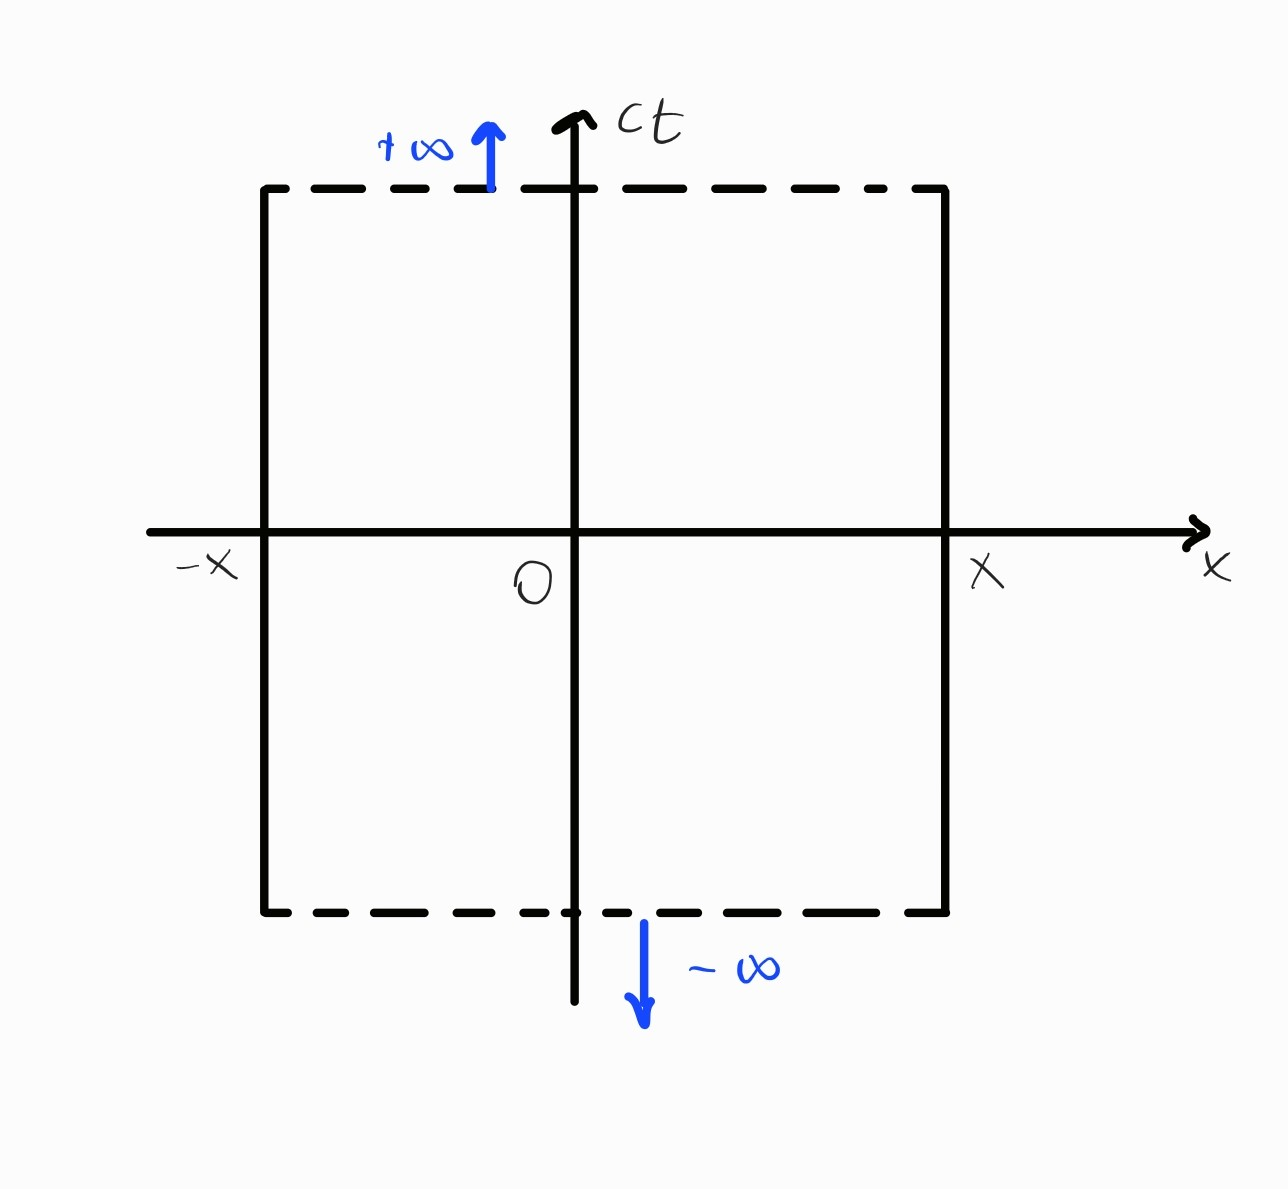
\includegraphics[width=5cm]{Immagini/Integrazione_temporale.jpg} }}%
    \qquad
    \subfloat[\centering Integrazione spaziale.]{{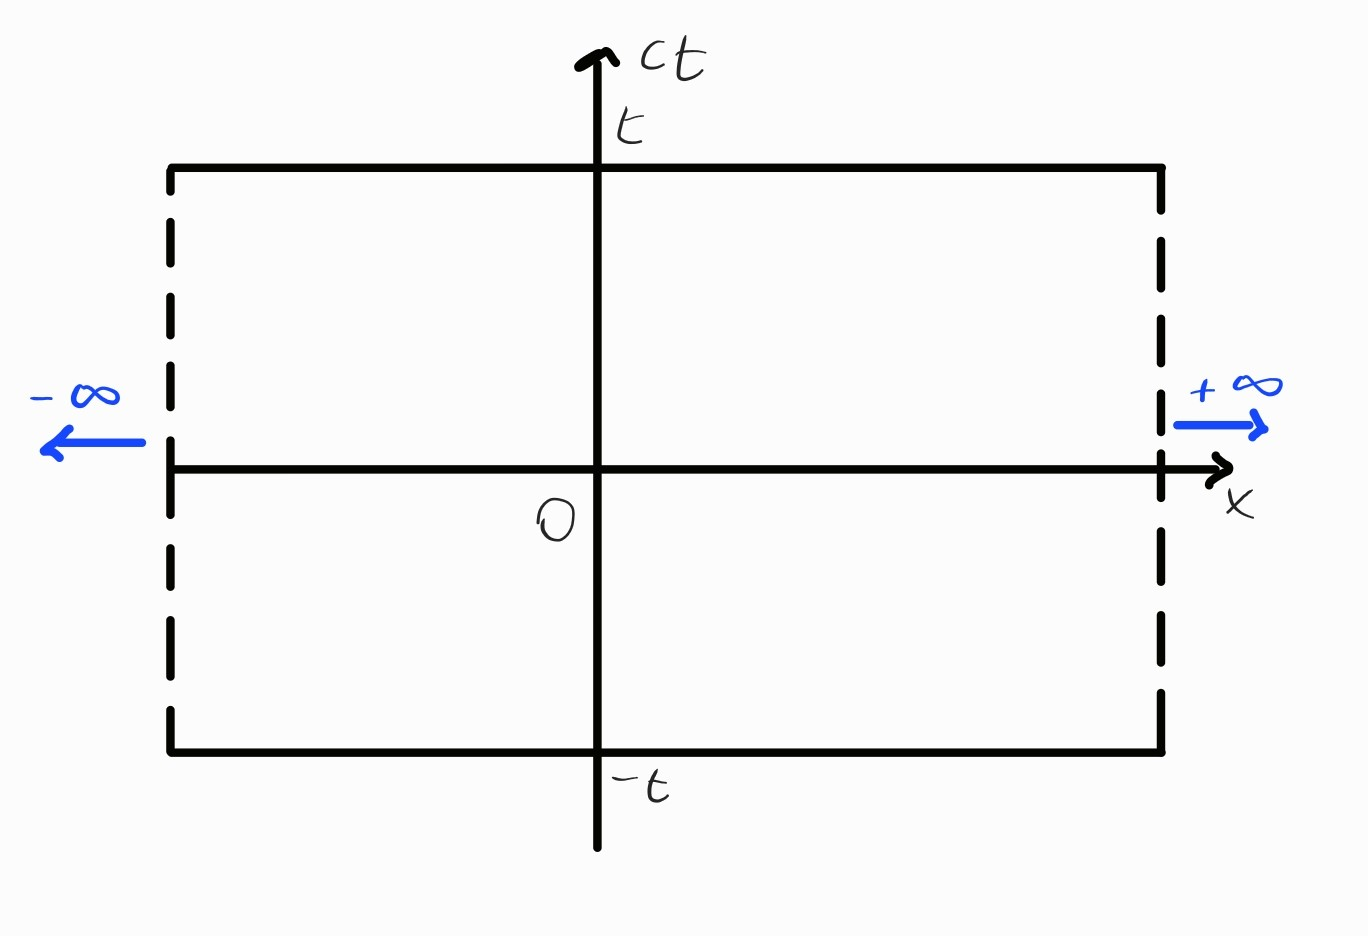
\includegraphics[width=5cm]{Immagini/Integrazione_spaziale.jpg} }}%
    \caption{Integrazione nello spazio di Minkowski.}%
    \label{fig:Int_inf}%
\end{figure}

\subsection{Potenziali di Lienard-Wiechert}
Consideriamo quanto appreso nella sezione \ref{sec:2.2} e applichiamolo al semplice caso di una carica in movimento, al fine di determinarne il potenziale.
Consideriamo la carica $e$ in moto vario lungo la traiettoria $z(t)$, come mostrato in Fig.\ref{fig:Carica}.
\begin{figure}[H]
    \centering
    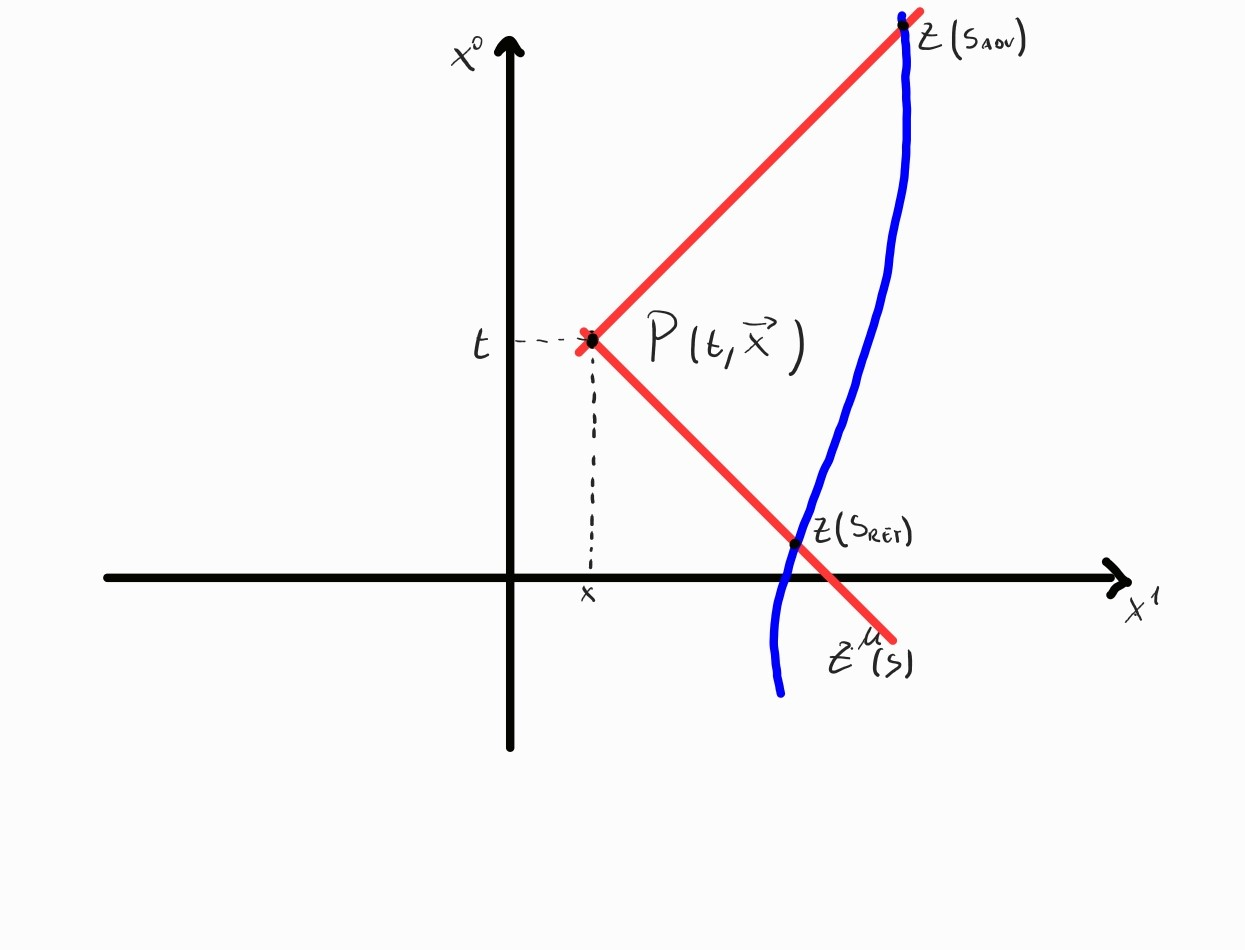
\includegraphics[width=0.36\textwidth]{Immagini/L-W.jpg}
    \caption{Carica in moto vario.}
    \label{fig:Carica}
\end{figure}
Consideriamo, dunque, la \eqref{eq:Maxwell_sorgenti_sol} e sostituiamoci la \eqref{eq:def_quad_corr2} e la \eqref{eq:Green_inva}:
\begin{equation}
\begin{aligned}
     A_{ret}^\alpha(t,\Vec{x})&=\dfrac{4\pi}{c}\int d^4x'D(x-x')j^\alpha(t',\Vec{x}')\\
     &=\dfrac{4\pi}{c}\int d^4x'[\dfrac{1}{2\pi}\delta\left((x-x')^2\right)\Theta(x_0-x'_0)][c\int ds \quad e\delta^4\left(x'-z(s)\right)u^\alpha]\\
     &=2e\iint  d^4x'\quad ds\quad \delta\left((x-x')^2\right)\Theta(x_0-x'_0)\delta^4\left(x'-z(s)\right)u^\alpha
\end{aligned}
\end{equation}
ove la sommatoria delle cariche scompare poiché ne consideriamo una sola. Inoltre, considerando la proprietà della delta $\int dx f(x)\delta(x-y)=f(y)$, quindi sostituiamo ad $x'$ la traiettoria $z(s)$:
\begin{equation}
\begin{aligned}
     A_{ret}^\alpha(t,\Vec{x})&=2e\int ds\quad \delta\left((x-z)^2\right)\Theta(x_0-z_0)u^\alpha(s)\\
     &=2e\int ds\quad \delta\left[(x^0-z^0)^2-|\Vec{x}-\Vec{z}|^2\right]\Theta(x_0-z_0)u^\alpha(s)
\end{aligned}
\end{equation}
ovviamente $x$ rappresenta il punto di osservazione, mentre $z(t)$ la posizione della particella. Perché la delta abbia supporto dobbiamo avere $(x-z)^2=(x_\mu-z_\mu)(x^\mu-z^\mu)=0$, ossia un vettore di tipo luce. Possiamo riscrivere la delta come:
\begin{equation}
     \delta\left[(x^0-z^0)^2-|\Vec{x}-\Vec{z}|^2\right]= \delta\left\{[(x^0-z^0)+|\Vec{x}-\Vec{z}|][(x^0-z^0)-|\Vec{x}-\Vec{z}|]\right\}
\end{equation}
ciò indica due poli, il primo termine rappresenta il polo nel futuro, mentre il secondo rappresenta il polo nel passato, come mostrato in Fig.\ref{fig:Carica}. Per ragioni di causalità, il contributo nel futuro sarà nullo.

Ricordiamo la proprietà $\delta(g(x))=\sum_i \dfrac{\delta(x-x_i)}{|\frac{dg}{dx}|_{x_i}}$, abbiamo che:
\begin{equation}
    \dfrac{d}{ds}\left[(x_\mu-z_\mu)(x^\mu-z^\mu)\right]=-2(x^\mu-z^\mu)\dfrac{dz_\mu}{ds}=-2(x^\mu-z^\mu)u_\mu
\end{equation}
quindi possiamo riscrivere la delta, considerando solo il polo ritardato, come:
\begin{equation}
    \delta\left((x-z)^2\right)\Theta(x_0-z_0)=\dfrac{\delta(s-s_{ret})}{2(x^\mu-z^\mu)u_\mu}
\end{equation}
sostituendolo nel potenziale, otteniamo:\begin{equation}\phantomsection\label{eq:pot_L-W_1}
     A_{ret}^\alpha(t,\Vec{x})=2e\int ds\quad \dfrac{\delta(s-s_{ret})}{2(x^\mu-z^\mu(s))u_\mu}u^\alpha=e\dfrac{u^\alpha}{(x^\mu-z^\mu(s))u_\mu}\biggm|_{s_{ret}}\end{equation}
Però così lo abbiamo espresso nel tempo proprio, vogliamo cambiare parametrizzazione e passare al tempo generico. Sappiamo che $z^\mu(s_{ret})=(ct_{ret},\Vec{z}(t_{ret}))$ e che l'evento generico è $x^\mu=(t,\Vec{x})$, allora:
\begin{equation}
    \begin{gathered}
        (x_\mu-z_\mu)(x^\mu-z^\mu)=0\\
        c^2(t-t_{ret})^2-|\Vec{x}-\Vec{z}|^2=c^2(t-t_{ret})^2-|\Vec{R}|^2=0\\
        \implies t_{ret}=t-\dfrac{R(t_{ret})}{c}
    \end{gathered}
\end{equation}
Ricordando la definizione della quadrivelocità \eqref{eq:def_qvel}, abbiamo che:
\begin{equation}
      (x^\mu-z^\mu)u_\mu=\gamma\left[(ct-ct_{ret})^2-\Vec{R}(t_{ret})\Vec{\beta}(t_{ret})\right]=\gamma(R-\Vec{R}\Vec{\beta})\biggm|_{t_{ret}}
\end{equation}
sostituendolo nella \eqref{eq:pot_L-W_1}, otteniamo le componenti del potenziale:
\begin{equation}\phantomsection\label{eq:pot_L-W_2}
\begin{cases}
     A_{ret}^0(t,\Vec{x})=e\dfrac{u^0}{\gamma(R-\Vec{R}\Vec{\beta})}\biggm|_{t_{ret}}=\dfrac{e}{(R-\Vec{R}\Vec{\beta})}\biggm|_{t_{ret}}
     \\
     \\
     \Vec{A}_{ret}(t,\Vec{x})=\dfrac{e}{c}\dfrac{\Vec{u}}{\gamma(R-\Vec{R}\Vec{\beta})}\biggm|_{t_{ret}}=\dfrac{e}{c^2}\dfrac{\Vec{v}}{(R-\Vec{R}\Vec{\beta})}\biggm|_{t_{ret}}
\end{cases}
\end{equation}
il potenziale trovato è detto \textit{potenziale di Lienard-Wiechert}.

A partire da questo potenziale è possibile ottenere le equazioni del campo elettrico e del campo magnetico generati dalla carica in moto vario. Le riportiamo per completezza, ma non le ricaveremo. Consideriamo il tensore elettromagnetico datoci dal lemma di Poincaré $F\indices{^{\mu\nu}}=\partial^\mu A\nu-\partial^\nu A\mu$, definiamo $\Vec{R}=\Vec{x}-\Vec{z}(t)$ e il versore $\hat{n}=\dfrac{\Vec{R}}{|\Vec{R}|}$, allora il campo elettrico è dato da:
\begin{equation}
    \Vec{E}(t,\Vec{x})=e\left\{\dfrac{(1-\beta^2)(\hat{n}-\Vec{\beta})}{R^2(1-\Vec{\beta}\hat{n})^3} \right\}_{ret}+\dfrac{e}{c}\left\{\dfrac{\hat{n}\times[(\hat{n}-\beta^2)\times \Vec{\dot{\beta}}]}{R^2(1-\Vec{\beta}\hat{n})^3} \right\}_{ret}
\end{equation}
osserviamo che il primo termine dipende solo dalla velocità, quindi descrive il campo per la particella in moto rettilineo uniforme, il secondo termine dipende anche dall'accelerazione, quindi compare se il moto è accelerato, inoltre è il responsabile dell'irraggiamento.

Mentre il campo magnetico segue da:
\begin{equation}
    \Vec{B}(t,\Vec{x})=\left(\hat{n}\times\Vec{E}\right)_{ret}
\end{equation}
\newpage

\section{Tensore Energia-Impulso}
\subsection{Tensore energia-impulso}
In maniera analoga a quanto fatto in sezione \ref{sec:2.2}, ove, considerando una distribuzione di cariche, abbiamo definito la densità di carica e la densità di corrente, per poi unirle in un unico oggetto, al fine di trovare l'equazione di continuità. Considerando, nello stesso modo, una distribuzione di carica associamo, per ogni carica, un quadrimpulso: 
\begin{equation}
    P^\alpha_n=\left(\dfrac{E_n}{c}, \Vec{P}_n\right)=(\gamma m_nc,\gamma m_n \Vec{v}_n)
\end{equation}
A partire da questo possiamo definire la densità di energia-impulso come:
\begin{equation}
    T^{\alpha0}=c\sum_nP^\alpha_n\delta^3(\Vec{x}-\Vec{x}_n)
\end{equation}
e una densità di corrente di energia-impulso:
\begin{equation}
    T^{\alpha i}=\sum_nP^\alpha_n\delta^3(\Vec{x}-\Vec{x}_n)\dfrac{dx^i_n}{dt}(t)
\end{equation}
Ora, definiamo il \textit{tensore energia-impulso} come l'unione di questi oggetti:
\begin{equation}\phantomsection\label{eq:def_tens_E-I}
    T^{\alpha \beta}=\sum_nP^\alpha_n\delta^3(\Vec{x}-\Vec{x}_n)\dfrac{dx^\beta_n}{dt}(t)
\end{equation}
dimostriamo rapidamente che il tensore energia-impulso è simmetrico.
\begin{proof}
    Dalla definizione di quadrimpulso abbiamo che la componente spaziale si può scrivere:
    \begin{equation}
      \Vec{P}=\dfrac{E\Vec{v}}{c^2} \quad \text{ da cui segue} \quad P^\beta_n=\dfrac{E_n}{c^2}\dfrac{dx^\beta_n}{dt}
    \end{equation}
    sostituendola nella \eqref{eq:def_tens_E-I}, otteniamo:
    \begin{equation}
    T^{\alpha \beta}=\sum_nP^\alpha_n\delta^3(\Vec{x}-\Vec{x}_n)P^\beta_n\dfrac{c^2}{E_n}=c^2\sum_n\dfrac{P^\alpha_nP^\beta_n}{E_n}\delta^3(\Vec{x}-\Vec{x}_n)
\end{equation}
In tale forma risulta evidente la simmetria.\\
\end{proof}
Dalla \eqref{eq:def_tens_E-I} non è, tuttavia, evidente che sia un tensore, perciò dimostriamolo brevemente:
\begin{proof}
    Partiamo dalla definizione ed utiliziamo una delta di Dirac nel tempo:
    \begin{equation}
  \begin{aligned}
      T^{\alpha \beta}&=\sum_nP^\alpha_n\dfrac{dx^\beta_n}{dt}(t)\delta^3(\Vec{x}-\Vec{x}_n)=\int dt'\sum_nP^\alpha_n\dfrac{dx^\beta_n}{dt'}(t')\delta(t-t')\delta^3(\Vec{x}-\Vec{x}_n)\\
      &=c\int ds\sum_nP^\alpha_n\dfrac{dx^\beta_n}{ds}(s)\delta^4(x-x')
  \end{aligned}
\end{equation}
In tale forma risulta evidente la natura tensoriale dell'oggetto.\\
\end{proof}
Possiamo riconoscere negli elementi del tensore delle quantità importanti: la componente $T^{00}$ è la densità di energia, gli elementi $T^{i0}$ sono le densità delle componenti i-esime dell'impulso, mentre gli elementi $T^{0i}$ sono la densità del flusso di energia lungo $x^i$ ed, infine, gli elementi del tensore $3\times3$ $T^{ij}$ sono dette componenti del tensore degli sforzi di Maxwell\footnote{Nei casi che noi considereremo il tensore sarà sempre simmetrico, tuttavia ci sono casi in cui non lo è; ci sono delle procedure per simmetrizzarlo che consistono nell'aggiunta di altri tensori. La ragione per cui si ricercano tensori energia-impulso simmetrici è che in relatività generale, nelle equazioni di campo di Einstein, il membro sinistro risulta simmetrico e il membro destro è il tensore energia-impulso (la sorgente).}.

Vogliamo, ora, determinare un'equazione di continuità. Per farlo consideriamo la divergenza di $T^{\alpha \beta}$ e utilizziamo la proprietà secondo cui se una funzione ha una dipendenza del tipo $F(x-y)$, allora vale l'identità $\dfrac{\partial F}{\partial x}=-\dfrac{\partial F}{\partial y}$:
  \begin{equation}
  \begin{aligned}
      \dfrac{\partial}{\partial x^i}T^{\alpha i}&=\sum_nP^\alpha_n(t)\dfrac{\partial x^i_n}{\partial t} \dfrac{\partial }{\partial x^i}\delta^3(\Vec{x}-\Vec{x}_n)=-\sum_nP^\alpha_n(t)\dfrac{\partial x^i_n}{\partial t} \dfrac{\partial}{\partial x^i_n}\delta^3(\Vec{x}-\Vec{x}_n)\\
      &=-\sum_nP^\alpha_n(t)\dfrac{\partial }{\partial t} \delta^3(\Vec{x}-\Vec{x}_n)=-\dfrac{1}{c}\dfrac{\partial T^{\alpha 0}}{\partial t}+\sum_n\dfrac{dP^\alpha_n}{dt}(t)\delta^3(\Vec{x}-\Vec{x}_n)
  \end{aligned}
\end{equation}
ove nell'ultimo passaggio, a causa della dipendenza del quadrimpulso dal tempo, consideriamo la derivata della delta come la sottrazione tra la derivata del prodotto meno la derivata rispetto a $P^\alpha_n$.
Riscriviamo l'ultima relazione come:
 \begin{equation}
 \dfrac{\partial}{\partial x^i}T^{\alpha i}+\dfrac{1}{c}\dfrac{\partial T^{\alpha 0}}{\partial t}=\sum_n\dfrac{dP^\alpha_n}{dt}(t)\delta^3(\Vec{x}-\Vec{x}_n)
\end{equation}
possiamo riscrivere l'equazione considerando la quadridivergenza
\begin{equation}\phantomsection\label{eq:Quaddiv_tens_E-I}
 \dfrac{d}{dx^\beta}T^{\alpha \beta}=\sum_n\delta^3(\Vec{x}-\Vec{x}_n)\dfrac{dP^\alpha_n}{dt}(t)
\end{equation}
Nel caso di particelle libere avremo che:
\begin{equation}
    \dfrac{dP^\alpha_n}{dt}=0 \implies\dfrac{d}{dx^\beta}T^{\alpha \beta}=0
\end{equation}
quindi, dalla definizione del tensore energia-impulso avremo che:
\begin{equation}
    P^\alpha=\int d^3x \quad T^{\alpha0}
\end{equation}
derivando nel tempo
\begin{equation}
 \dfrac{1}{c}  \dfrac{dP^\alpha}{dt}=\int d^3x\quad \dfrac{1}{c} \partial_t T^{\alpha0}=-\int d^3x \quad\partial_i T^{\alpha i}=-\int_\Sigma d\Sigma\quad T^{\alpha i}=0
\end{equation}
ove nell'ultimo passaggio si è utilizzato il teorema di Gauss. Concludiamo che in questo caso particolare il quadrimpulso è conservato, tuttavia dalla \eqref{eq:Quaddiv_tens_E-I} in generale sembrerebbe di no. La questione risulta essere problematica. Per  risolverla bisogna considerare gli scambi tra particelle e campo, sarà il quadrimpulso totale a doversi conservare.
\subsection{Particelle cariche in un campo elettromagnetico}
Sulla base di quanto appreso nel precedente capitolo, applichiamo le nuove conoscenze al caso di particelle immerse in un campo elettromagnetico. Ricordiamo, dallo studio della dinamica in sezione \ref{sec:2.1}, che la forza di Lorentz è:
\begin{equation}
     \dfrac{dP^\alpha}{ds}=\dfrac{e_n}{c}F^{\alpha\beta}u_\beta
\end{equation}
questa relazione considera una sola carica, ovviamente per rendere il conto generale bisogna considerare una sommatoria nelle n.
Possiamo riscrivere la relazione precedente in funzione di $dt$ e attraverso la matrice metrica possiamo alzare ed abbassare indici
\begin{equation}
\begin{gathered}
     \dfrac{dP^\alpha}{dt}\dfrac{dt}{ds}=\dfrac{e_n}{c}F^\alpha_\beta u^\beta=\dfrac{e_n}{c}F^\alpha_\beta \dfrac{dx_n^\beta}{dt}\dfrac{dt}{ds}\\
     \implies\dfrac{dP^\alpha}{dt}=\dfrac{e_n}{c}F^\alpha_\beta \dfrac{dx_n^\beta}{dt}
\end{gathered}
\end{equation}
sostituendo nella \eqref{eq:Quaddiv_tens_E-I} otteniamo il tensore energia impulso del sistema di particelle:
\begin{equation}\phantomsection\label{eq:tens_par}
 \dfrac{d}{dx^\beta}T^{\alpha \beta}_{par}=\sum_n\dfrac{e_n}{c}F^\alpha_\gamma \dfrac{dx_n^\gamma}{dt}\delta^3(\Vec{x}-\Vec{x}_n)=\dfrac{1}{c}F^\alpha_\gamma j^\gamma
\end{equation}
quindi il quadrimpulso non si conserva, ma ricordiamo, questo è il quadrimpulso delle particelle. Quello che il buon senso fisico suggerisce è che sia il quadrimpulso totale, comprendente anche del quadrimpulso del campo a conservarsi $P^\alpha_T=P^\alpha_{par}+P^\alpha_{cam}$, ossia $\dfrac{dP^\alpha_T}{dt}=0$.

Possiamo introdurre il tensore energia-impulso del campo elettromagnetico:
\begin{equation}
 T^{\alpha \beta}_{cam}=-\dfrac{1}{4\pi}\left(F^\alpha_\gamma F^{\beta\gamma}- \dfrac{1}{4}\eta^{\alpha\beta}F_{\gamma\delta} F^{\gamma\delta} \right)
\end{equation}
notiamo che le componenti 
\begin{equation}
    \begin{gathered}
        T^{00}_{cam}=\dfrac{1}{8\pi}(E^2+B^2)\\
        T^{0i}_{cam}=\dfrac{1}{4\pi}(\Vec{E}\times\Vec{B})_i
    \end{gathered}
\end{equation}
sono, rispettivamente, la densità di energia del campo elettromagnetico e il vettore di Poynting. 

 Come già dimostrato in generale, il tensore è simmetrico $T^{\alpha \beta}_{cam}=T^{\beta \alpha}_{cam}$, un'altra proprietà interessante è che ha traccia nulla, per mostrarlo abbassiamo un indice e contraiamolo:
\begin{equation}
 T\indices{_{cam}^\alpha_\alpha}=-\dfrac{1}{4\pi}\left(F^\alpha_\gamma F^\gamma_\alpha- \dfrac{1}{4}\delta^\alpha_\alpha F_{\gamma\delta} F^{\gamma\delta} \right)=-\dfrac{1}{4\pi}\left(F^{\alpha\gamma} F_{\gamma\alpha}- F_{\gamma\delta} F^{\gamma\delta} \right)=0
\end{equation}
ove $\delta^\alpha_\gamma=4$ poiché siamo in uno spazio quadridimensionale, in altre dimensioni non è detto che la traccia sia nulla. Ora calcoliamoci la quadridivergenza:
\begin{equation}
\begin{aligned}
\dfrac{d}{dx^\beta}T^{\alpha\beta}_{cam}&=-\dfrac{1}{4\pi}\left[\partial_\beta(F^\alpha_\gamma)F^{\beta\gamma}+F^\alpha_\gamma\partial_\beta(F^{\beta\gamma})- \dfrac{1}{4}\partial_\beta(\eta^{\alpha\beta}F_{\gamma\delta} F^{\gamma\delta}) \right]\\
&=-\dfrac{1}{4\pi}\left[\partial_\beta(F^\alpha_\gamma)F^{\beta\gamma}+F^\alpha_\gamma\partial_\beta(F^{\beta\gamma})- \dfrac{1}{4}\partial^\alpha(F_{\gamma\delta} F^{\gamma\delta}) \right]\\
&=-\dfrac{1}{4\pi}\left[\partial^\beta(F^{\alpha\gamma})F_{\beta\gamma}+F^\alpha_\gamma\partial_\beta(F^{\beta\gamma})- \dfrac{1}{4}\partial^\alpha(F_{\gamma\delta}) F^{\gamma\delta}- \dfrac{1}{4}\partial^\alpha(F^{\gamma\delta}) F_{\gamma\delta} \right]\\
&\text{Riconosciamo nel secondo termine, l'equazione di Maxwell non omogenea \eqref{eq:eq_non_omo}:}
\\
\dfrac{d}{dx^\beta}T^{\alpha\beta}_{cam}&=-\dfrac{1}{4\pi}\left[\partial^\beta(F^{\alpha\gamma})F_{\beta\gamma}+F^\alpha_\gamma\dfrac{4\pi}{c}j^\gamma- \dfrac{1}{4}\partial^\alpha(F^{\gamma\delta}) F_{\gamma\delta} - \dfrac{1}{4}\partial^\alpha(F^{\gamma\delta}) F_{\gamma\delta}  \right]\\
&=-\dfrac{1}{c}F^\alpha_\gamma j^\gamma-\dfrac{1}{4\pi}\left[\partial^\beta(F^{\alpha\gamma})F_{\beta\gamma}- \dfrac{1}{2}\partial^\alpha(F^{\gamma\delta}) F_{\gamma\delta}   \right]\\
&\text{nell'ultimo termine $\delta$ è un indice di sommatoria, possiamo ribattezzarlo $\beta$}\\
\dfrac{d}{dx^\beta}T^{\alpha\beta}_{cam}&=-\dfrac{1}{c}F^\alpha_\gamma j^\gamma-\dfrac{1}{4\pi}\left[\partial^\beta(F^{\alpha\gamma})F_{\beta\gamma}- \dfrac{1}{2}\partial^\alpha(F^{\gamma\beta}) F_{\gamma\beta}   \right]
\end{aligned}
\end{equation}
studiamo i termini rimasti dentro la quadra, al fine di dimostrare che è nulla. Partiamo dal primo termine:
\begin{equation}
\begin{aligned}
\partial^\beta(F^{\alpha\gamma})&=\dfrac{2}{2}\partial^\beta(F^{\alpha\gamma})+\dfrac{1}{2}\partial^\gamma(F^{\alpha\beta})-\dfrac{1}{2}\partial^\gamma(F^{\alpha\beta})\\
&=\dfrac{1}{2}(\partial^\beta F^{\alpha\gamma}+\partial^\gamma F^{\alpha\beta})+\dfrac{1}{2}(\partial^\beta F^{\alpha\gamma}-\partial^\gamma F^{\alpha\beta})
\end{aligned}
\end{equation}
notiamo che il primo termine è simmetrico per lo scambio $\beta\leftrightarrow\gamma$ mentre il secondo è antisimmetrico, quindi moltiplicandolo per il tensore elettromagnetico, il quale è antisimmetrico, sopravvive solo il termine antisimmetrico ed otteniamo:
\begin{equation}
\begin{aligned}
\partial^\beta(F^{\alpha\gamma})F_{\beta\gamma}&=+\dfrac{1}{2}(\partial^\beta F^{\alpha\gamma}-\partial^\gamma F^{\alpha\beta})F_{\beta\gamma}
\end{aligned}
\end{equation}
sostituendo quest'ultimo risultato nella quadra troviamo:
\begin{equation}
\begin{aligned}
\dfrac{d}{dx^\beta}T^{\alpha\beta}_{cam}&=-\dfrac{1}{c}F^\alpha_\gamma j^\gamma-\dfrac{1}{4\pi}\left[\dfrac{1}{2}(\partial^\beta F^{\alpha\gamma}-\partial^\gamma F^{\alpha\beta})F_{\beta\gamma}-\dfrac{1}{2}\partial^\alpha(F^{\gamma\beta}) F_{\gamma\beta}   \right]\\
&=-\dfrac{1}{c}F^\alpha_\gamma j^\gamma-\dfrac{1}{4\pi}\left[\dfrac{1}{2}(\partial^\beta F^{\alpha\gamma}-\partial^\gamma F^{\alpha\beta})F_{\beta\gamma}+\dfrac{1}{2}\partial^\alpha(F^{\gamma\beta}) F_{\beta\gamma}   \right]\\
&=-\dfrac{1}{c}F^\alpha_\gamma j^\gamma-\dfrac{1}{8\pi}\left[\partial^\beta F^{\alpha\gamma}-\partial^\gamma F^{\alpha\beta} +\partial^\alpha F^{\gamma\beta}   \right]F_{\beta\gamma}\\
&=-\dfrac{1}{c}F^\alpha_\gamma j^\gamma-\dfrac{1}{8\pi}\left[\partial^\beta F^{\alpha\gamma}+\partial^\gamma F^{\beta\alpha} +\partial^\alpha F^{\gamma\beta}   \right]F_{\beta\gamma}\\
\end{aligned}
\end{equation}
dall'equazione \eqref{eq:omo_no_duale} otteniamo
\begin{equation}\phantomsection\label{eq:tens_camp}
\dfrac{d}{dx^\beta}T^{\alpha\beta}_{cam}=-\dfrac{1}{c}F^\alpha_\gamma j^\gamma
\end{equation}

A questo punto possiamo definire il tensore energia-impulso totale e sostituendo le \eqref{eq:tens_par} \eqref{eq:tens_camp}:
\begin{equation}\phantomsection\label{eq:tens_cont}
T^{\alpha\beta}_T=T^{\alpha\beta}_{par}+T^{\alpha\beta}_{cam} \implies\dfrac{d}{dx^\beta}T^{\alpha\beta}_T=\dfrac{d}{dx^\beta}T^{\alpha\beta}_{par}+\dfrac{d}{dx^\beta}T^{\alpha\beta}_{cam}=0
\end{equation}
da cui segue che 
\begin{equation}
P^{\alpha}_T=P^{\alpha}_{par}+P^{\alpha}_{cam}=\int d^3x\quad T^{\alpha0}_{par}+T^{\alpha0}_{cam}
\end{equation}
si conserva.

\subsection{Fluidi perfetti}

Il tensore energia-impulso è particolarmente usato nei modelli della fisica che si basano sui, così detti, \textit{fluidi perfetti}. Moltissimi sistemi fisici possono essere descritti, con opportune approssimazioni, come fluidi. I fluidi perfetti sono modellizzazioni ideali di fluidi con viscosità nulla e senza capacità di condurre calore\footnote{Ciò significa che il flusso del fluido è legato solo al moto delle particelle che lo costituiscono.}. Consideriamo un fluido in movimento, in particolare definiamo un sistema di riferimento comovente con il fluido, si veda Fig.\ref{fig:fluido}. 
\begin{figure}[H]
    \centering
    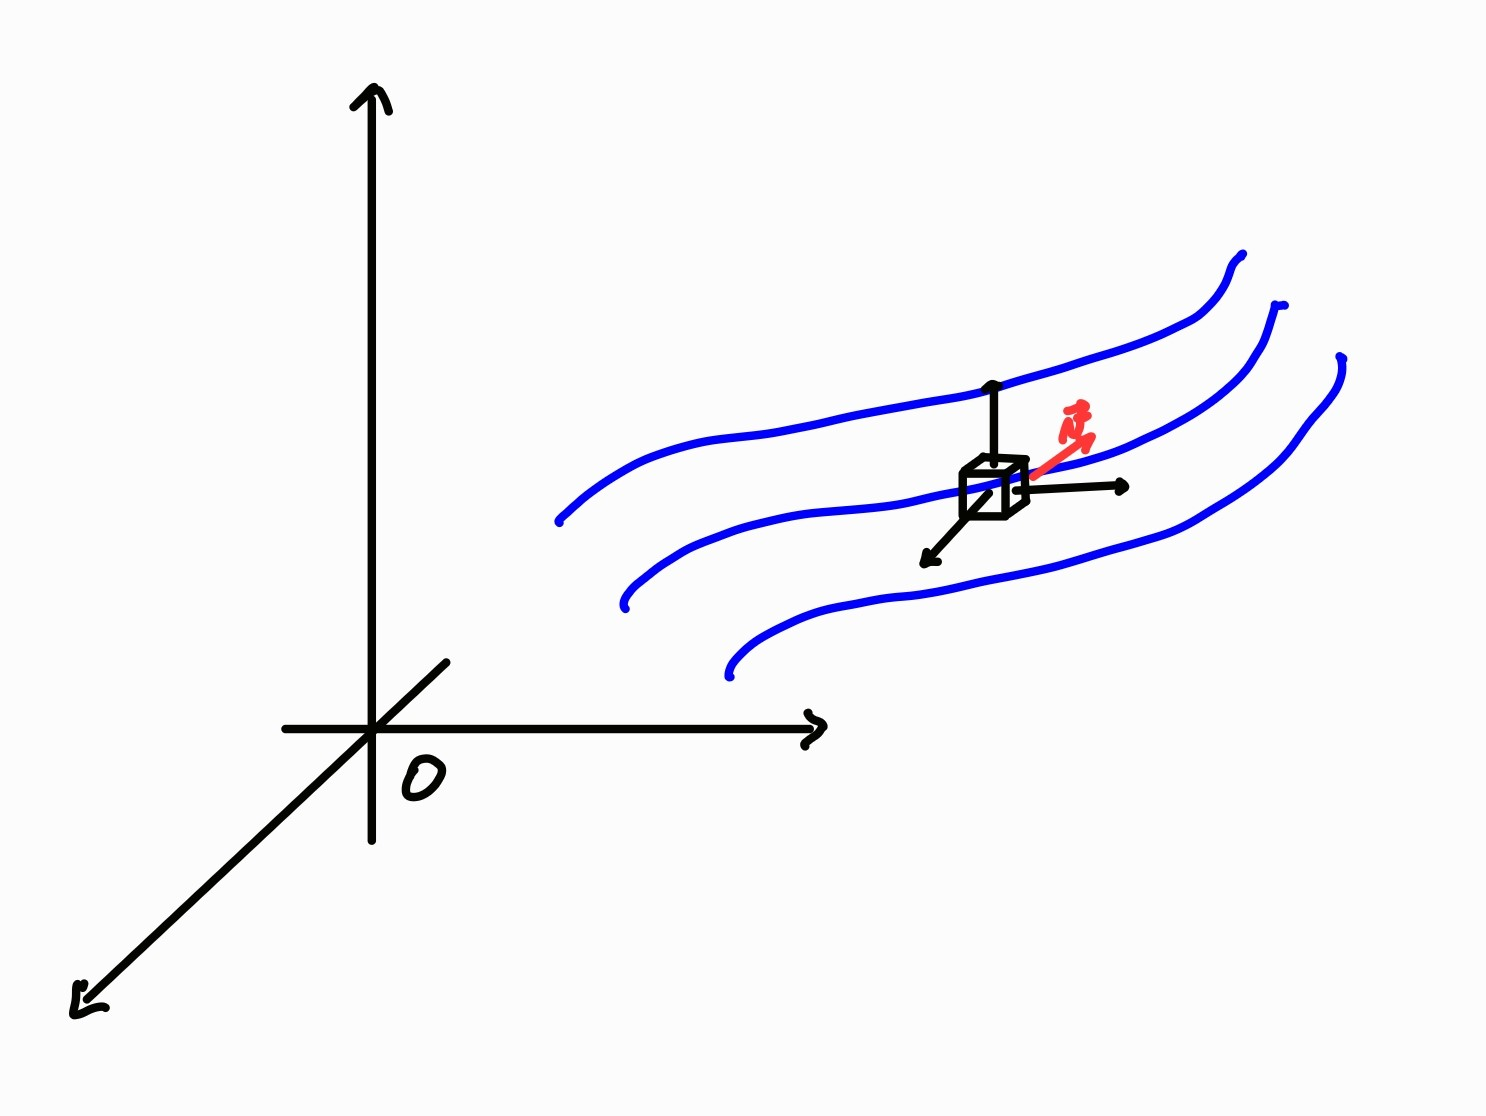
\includegraphics[width=0.31\textwidth]{Immagini/Fluido.jpg}
    \caption{Fluido perfetto in moto.}
    \label{fig:fluido}
\end{figure}
In tale sistema il tensore energia-impulso associato al fluido deve essere isotropo ed  assume la semplice forma:
\begin{equation}
\Tilde{T}\indices{^\gamma_\beta}=
\begin{pmatrix}
  \rho & 0 & 0 & 0  \\
  0 & p & 0 & 0  \\
  0 & 0 & p & 0   \\
  0 & 0 & 0 & p
\end{pmatrix}
\end{equation}
ove $\rho$ è la densità di energia e $p$ la pressione nel sistema comovente\footnote{Osserviamo che ai sistemi è associabile un'equazione di stato. Un esempio semplice si ha quando l'equazione di stato è  $p=0$, anche detta della polvere.}. Mentre in un sistema fisso, per esempio di un laboratorio, il sistema comovente avrà una certa velocità $\Vec{v}$, in generale, variabile localmente. Ci aspettiamo che la trasformazione che leghi i tensori energia-impulso sia una trasformazione di Lorentz:
\begin{equation}
T\indices{^{\alpha\beta}}=\Lambda\indices{^\alpha_\mu}(-\Vec{v})\Lambda\indices{^\beta_\nu}(-\Vec{v})\Tilde{T}\indices{^{\mu\nu}}
\end{equation}
ricordiamo che, in generale, la matrice di trasformazione ha le componenti \eqref{eq:generic_elem_tras}. 

Determiniamo le componenti del tensore energia-impulso nel sistema generico:
\begin{equation}
\begin{aligned}
    T^{00}&=\Lambda\indices{^0_\mu}\Lambda\indices{^0_\nu}\Tilde{T}\indices{^{\mu\nu}}=\Lambda\indices{^0_0}\Lambda\indices{^0_0}\Tilde{T}\indices{^{00}}+\Lambda\indices{^0_i}\Lambda\indices{^0_j}\Tilde{T}\indices{^{ij}}=\gamma^2\rho+\gamma^2\beta_i\beta_jp\delta_{ij}\\
    &=\gamma^2(\rho+\beta^2p)=\gamma^2\rho+\gamma^2\beta^2p=\gamma^2\rho+\dfrac{\beta^2}{1-\beta^2}p=\gamma^2\rho+(\gamma^2-1)p=\gamma^2(\rho+p)-p
    \end{aligned}
\end{equation}
consideriamo ora le componenti:
\begin{equation}
\begin{aligned}
   T^{i0}= T^{0i}&=\Lambda\indices{^0_\mu}\Lambda\indices{^i_\nu}\Tilde{T}\indices{^{\mu\nu}}=\Lambda\indices{^0_0}\Lambda\indices{^i_0}\Tilde{T}\indices{^{i0}}+\Lambda\indices{^0_j}\Lambda\indices{^i_k}\Tilde{T}\indices{^{jk}}=\gamma^2\beta_i\rho+\beta_j\gamma\left[\delta_{ik}+(\gamma-1)\dfrac{\beta_i\beta_k}{\beta^2}\right]p\delta_{jk}\\
   &=\gamma^2\beta_i\rho+\beta_j\gamma\left[\delta_{ij}+(\gamma-1)\dfrac{\beta_i\beta_j}{\beta^2}\right]p=\gamma^2\beta_i\rho+\beta_i\gamma p+\gamma(\gamma-1)\dfrac{\beta^2\beta_i}{\beta^2}p\\
   &=\gamma^2\beta_i\rho+\beta_i\gamma p+(\gamma^2-\gamma)\beta_ip=\gamma^2\beta_i(\rho+p)
    \end{aligned}
\end{equation}
infine rimane:
\begin{equation}
\begin{aligned}
   T^{ij}&=\Lambda\indices{^i_\mu}\Lambda\indices{^j_\nu}\Tilde{T}\indices{^{\mu\nu}}=\Lambda\indices{^i_0}\Lambda\indices{^j_0}\Tilde{T}\indices{^{i0}}+\Lambda\indices{^i_k}\Lambda\indices{^j_l}\Tilde{T}\indices{^{kl}}\\
   &=\gamma^2\beta_i\beta_j\rho+\left[\delta_{ik}+(\gamma-1)\dfrac{\beta_i\beta_k}{\beta^2}\right]\left[\delta_{jl}+(\gamma-1)\dfrac{\beta_j\beta_l}{\beta^2}\right]p\delta_{kl}\\
   &=\gamma^2\beta_i\beta_j\rho+\left[\delta_{ij}+(\gamma-1)\dfrac{\beta_i\beta_j}{\beta^2}+(\gamma-1)\dfrac{\beta_i\beta_j}{\beta^2}+(\gamma-1)^2\dfrac{(\beta_i\beta_j)(\beta_k\beta_k)}{\beta^2\beta^2}\right]p\\
   &=\gamma^2\beta_i\beta_j\rho+\left\{\delta_{ij}+\dfrac{\beta_i\beta_j}{\beta^2}[2(\gamma-1)+(\gamma-1)^2]\right\}p\\
   &=\gamma^2\beta_i\beta_j\rho+\left\{\delta_{ij}+\dfrac{\beta_i\beta_j}{\beta^2}[2(\gamma-1)+(\gamma^2-2\gamma+1)]\right\}p\\
   &=\gamma^2\beta_i\beta_j\rho+\left[\delta_{ij}+\dfrac{\beta_i\beta_j}{\beta^2}(\gamma^2-1)\right]p=\gamma^2\beta_i\beta_j\rho+\left[\delta_{ij}+\dfrac{\beta_i\beta_j}{\beta^2}(\dfrac{1}{1-\beta^2}-1)\right]p\\
   &=\gamma^2\beta_i\beta_j\rho+\left[\delta_{ij}+\dfrac{\beta_i\beta_j}{\beta^2}\left(\dfrac{\beta^2}{1-\beta^2}\right)\right]p=\gamma^2\beta_i\beta_j\rho+\left[\delta_{ij}+\dfrac{\beta_i\beta_j}{1-\beta^2}\right]p\\
   &=\gamma^2\beta_i\beta_j\rho+\delta_{ij}p+\gamma^2\beta_i\beta_jp=\gamma^2\beta_i\beta_j(\rho+p)+\delta_{ij}p
   \end{aligned}
\end{equation}
A partire da queste tre relazioni vogliamo scrivere una sola equazione covariante. Per farlo, consideriamo la quadrivelocità $u^\mu=(\gamma,\gamma\Vec{\beta})$ e riscriviamo tutte le relazioni precedenti:
\begin{equation}
     T^{00}=\gamma^2(\rho+p)-p=(\rho+p)u^0u^0-\eta^{00}p
\end{equation}
\begin{equation}
     T^{i0}=\gamma^2\beta_i(\rho+p)=(\rho+p)u^0u^i
\end{equation}
\begin{equation}
    T^{ij}=\gamma^2\beta_i\beta_j(\rho+p)+\delta_{ij}p=(\rho+p)u^iu^j-\eta^{ij}p
\end{equation}
concludiamo che la forma covariante compatta è:\begin{equation}\phantomsection\label{eq:tensore_fluidi}
    T^{\mu\nu}=(\rho+p)u^\mu u^\nu -\eta^{\mu\nu}p
\end{equation}
Consideriamo, ora, che il sistema sia isolato e quindi:
\begin{equation}
\begin{gathered}
    \dfrac{dT^{\alpha\beta}}{dx^\beta}=0 \\ 
    \dfrac{d}{dx^\beta}[(\rho+p)u^\alpha u^\beta]-\dfrac{d}{dx^\beta}[\eta^{\alpha\beta}p]=0\\
    \dfrac{d}{dx^\beta}[(\rho+p)u^\alpha u^\beta]-\dfrac{dp}{dx_\alpha}=0
\end{gathered}
\end{equation}
ove nell'ultimo passaggio si è utilizzata la proprietà di innalzamento di indice per la derivata; la relazione è ovviamente vettoriale, dunque consideriamo componente per componente. 

Fissiamo $\alpha=0$ e notiamo che $u^j=u^0\beta^j$:
\begin{equation}\phantomsection\label{eq:alfa_0}
\begin{gathered}
   \dfrac{d}{dx^\beta}[(\rho+p)u^0 u^\beta]-\dfrac{dp}{dx_0}=0\\
  \dfrac{1}{c} \dfrac{d}{dt}[(\rho+p)u^0 u^0]+ \dfrac{d}{dx^j}[(\rho+p)u^0 u^j]-\dfrac{1}{c}\dfrac{dp}{dt}=0\\
   \dfrac{1}{c}\dfrac{d}{dt}[(\rho+p)(u^0)^2]+ \dfrac{d}{dx^j}[(\rho+p)(u^0)^2 \frac{v^j}{c}]-\dfrac{1}{c}\dfrac{dp}{dt}=0
\end{gathered}
\end{equation}
ora consideriamo $\alpha=i$ (ossia le coordinate spaziali):
\begin{equation}
\begin{gathered}
   \dfrac{d}{dx^\beta}[(\rho+p)u^i u^\beta]-\dfrac{dp}{dx_i}=0\\
   \dfrac{d}{dx^0}[(\rho+p)u^i u^0]+\dfrac{d}{dx^j}[(\rho+p)u^i u^j]-\dfrac{dp}{dx_i}=0\\
    \dfrac{1}{c}\dfrac{d}{dt}[(\rho+p)(u^0)^2\frac{v^i}{c}]+\dfrac{d}{dx^j}[(\rho+p)(u^0)^2\frac{v^i}{c}\frac{v^j}{c}]+\dfrac{dp}{dx^i}=0\\
\end{gathered}
\end{equation}

    \begin{equation*}
          \dfrac{1}{c^2}\dfrac{dv^i}{dt}[(\rho+p)(u^0)^2]+\dfrac{v^i}{c^2}\dfrac{d}{dt}[(\rho+p)(u^0)^2]+\dfrac{1}{c^2}\dfrac{dv^i}{dx^j}[(\rho+p)(u^0)^2v^j]+\dfrac{v^i}{c^2}\dfrac{d}{dx^j}[(\rho+p)(u^0)^2v^j]+\dfrac{dp}{dx^i}=0\\
    \end{equation*}
      

usando la \eqref{eq:alfa_0} otteniamo $ \dfrac{1}{c}\dfrac{d}{dt}[(\rho+p)(u^0)^2]=+\dfrac{1}{c}\dfrac{dp}{dt}- \dfrac{1}{c}\dfrac{d}{dx^j}[(\rho+p)(u^0)^2 v^j]$, che sostituendola nella precedente:
\begin{equation*}
\begin{aligned}
    \dfrac{1}{c^2}\dfrac{dv^i}{dt}[(\rho+p)(u^0)^2]&+\dfrac{v^i}{c}\left\{+\dfrac{1}{c}\dfrac{dp}{dt}- \dfrac{1}{c}\dfrac{d}{dx^j}[(\rho+p)(u^0)^2 v^j]\right\}\\
    &+\dfrac{1}{c^2}\dfrac{dv^i}{dx^j}[(\rho+p)(u^0)^2v^j]+\dfrac{v^i}{c^2}\dfrac{d}{dx^j}[(\rho+p)(u^0)^2v^j]+\dfrac{dp}{dx^i}=0
\end{aligned}
\end{equation*}
\begin{equation}
\begin{aligned}
        \dfrac{1}{c^2}\dfrac{dv^i}{dt}[(\rho+p)(u^0)^2]&+\dfrac{v^i}{c^2}\dfrac{dp}{dt}-\dfrac{v^j}{c^2} \dfrac{d}{dx^j}[(\rho+p)(u^0)^2 v^j]\\
    &+\dfrac{1}{c^2}\dfrac{dv^i}{dx^j}[(\rho+p)(u^0)^2v^j]+\dfrac{v^i}{c^2}\dfrac{d}{dx^j}[(\rho+p)(u^0)^2v^j]+\dfrac{dp}{dx^i}=0
\end{aligned}
\end{equation}
\begin{equation*}
        \dfrac{1}{c^2}\dfrac{dv^i}{dt}[(\rho+p)(u^0)^2]+\dfrac{v^i}{c^2}\dfrac{dp}{dt}+\dfrac{1}{c^2}\dfrac{dv^i}{dx^j}[(\rho+p)(u^0)^2v^j]+\dfrac{dp}{dx^i}=0
\end{equation*}

dividiamo tutto per $[(\rho+p)(u^0)^2]$ e riordiniamo i termini:
\begin{equation}
\begin{gathered}
     \dfrac{\dfrac{dp}{dx^i}+\dfrac{v^i}{c^2}\dfrac{dp}{dt}}{[(\rho+p)(u^0)^2]} + \dfrac{1}{c^2}\dfrac{dv^i}{dt}+\dfrac{1}{c^2}\dfrac{dv^i}{dx^j}v^j=0\\
    -  \dfrac{\dfrac{dp}{dx^i}+\dfrac{v^i}{c^2}\dfrac{dp}{dt}}{[(\rho+p)(u^0)^2]}= + \dfrac{1}{c^2}\dfrac{dv^i}{dt}+\dfrac{1}{c^2}\dfrac{dv^i}{dx^j}v^j
\end{gathered}
\end{equation}
riscrivendola in forma vettoriale:
\begin{equation}\phantomsection\label{eq:euler_rel}
     -\dfrac{1-\frac{v^2}{c^2}}{\rho+p} \left[\Vec{\nabla}p+\dfrac{\Vec{v}}{c^2}\dfrac{\partial p}{\partial t}\right] =\dfrac{1}{c^2}\dfrac{d\Vec{v}}{dt}+\dfrac{1}{c^2}(\Vec{\nabla}\Vec{v})\Vec{v}
\end{equation}

La relazione appena trovata è \textit{l'equazione di Eulero relativistica}, il limite non relativistico si ha per $c>>v$ e $\rho>>p$.

Riassumiamo quanto fatto: siamo partiti dall'equazione di continuità del tensore energia-impulso e siamo giunti all'equazione del moto, quindi nella \eqref{eq:tens_cont} è racchiusa la dinamica locale del sistema.\footnote{Da notare che nel caso corrente è stato dimostrato per i fluidi perfetti, ma quest'ultima considerazione ha una valenza del tutto generale.}
\newpage

\section{Teoria dei Gruppi}
\subsection{Definizioni}

Diamo la definizione di \textit{gruppo}:

un gruppo $G$ è un insieme di elementi $\{g_i\}$ dotato di un legge di composizione interna $\cdot$ che gode delle seguenti proprietà:
\begin{enumerate}
    \item chiusura: $\forall g_i,g_j\in G \quad:\quad g_i\cdot g_j\in G$;
    \item associatività: $g_i\cdot (g_j\cdot g_k)=g_k\cdot (g_i\cdot g_j)$;
    \item identità: $\forall g_i\in G, \quad\exists g_0\in G \quad : \quad  g_i\cdot g_0= g_0\cdot g_i=g_i $;
    \item inverso: $\forall g_i\in G, \quad\exists g_i^{-1}\in G \quad : \quad  g_i\cdot g_i^{-1}= g_i^{-1}\cdot g_i=g_0$.
\end{enumerate}
inoltre, se vale la proprietà commutativa $g_i\cdot g_j=g_j\cdot g_i$ il gruppo $G$ è detto \textit{abeliano}.

Definiamo una \textit{rappresentazione del gruppo} come un insieme di di operatori lineari $\{T_i\}$, il quale è un omomorfismo che associa ad ogni elemento del gruppo un operatore lineare.

Quindi, $\forall g_i\in G\xrightarrow{omo}T(g_i):L\xrightarrow{}L$, ove $L$ è uno spazio lineare. Gli operatori riproducono le proprietà del gruppo di partenza:
\begin{enumerate}
    \item  $T(g_i)T(g_j)=T(g_i\cdot g_j)\qquad\forall i,j$;
    \item $T(g_0)=\mathds{I}$;
    \item  $T(g_i^{-1})=T^{-1}(g_i) \qquad\forall i$.
\end{enumerate}
Inoltre, diremo che la dimensione della rappresentazione è pari alla dimensione dello spazio vettoriale. Le rappresentazioni si caratterizzano per quelle finite dimensionali e per quelle infinite dimensionali.

\subsection{Gruppo per rotazioni}
I primi gruppi di interesse in fisica sono quelli che rappresentano rotazioni. In particolare, in forma matriciale e vettoriale abbiamo:
\begin{equation}
\begin{pmatrix}
x'   \\
y'   \\
 z'  \\
\end{pmatrix}
=R\begin{pmatrix}
x \\
y   \\
 z  \\
\end{pmatrix}\qquad
\Vec{r'}=R\Vec{r}
\end{equation}
ove $R$ è una matrice $3\times3$. Sotto rotazioni sappiamo che deve preservare l'invariante:
\begin{equation}
\begin{gathered}
    x'^2+y'^2+z'^2=x^2+y^2+z^2 \implies \Vec{r'}^T\Vec{r'}=\Vec{r}^T\Vec{r}\implies\\
    \Vec{r}^TR^TR\Vec{r}=\Vec{r}^T\Vec{r}\implies R^TR=\mathds{I}\implies R^T=R^{-1}
\end{gathered}
\end{equation}
Matrici $3\times3$ di questo tipo sono dette \textit{ortogonali}. Tutte le proprietà della definizione di gruppo sono soddisfatte, quindi definiamo il gruppo $O(3)$ di matrici ortogonali $\{R\}$.

Considerando il determinante della relazione matriciale precedente:
\begin{equation}   \det\left[R^TR\right]=1\implies \det\left[R\right]^2=1 \implies \det\left[R\right]=\pm1
\end{equation}
se il determinate è $-1$ si ha l'inversione spaziale, ossia una trasformazione discreta, che è la parità. Mentre per determinate pari a $1$ si hanno le trasformazioni dette speciali e il gruppo associato è $SO(3)$.
Noi ci limiteremo a quest'ultimo gruppo.

Consideriamo l'esempio di una rotazione nel piano $x-y$: 
\begin{equation}
    \Vec{v}'=R_z(\theta)\Vec{v}\qquad
    \begin{pmatrix}
v_x'   \\
v_y'   \\
 v_z'  \\
\end{pmatrix}
=    \begin{pmatrix}
 \cos{\theta}&\sin{\theta}&0  \\
  -\sin{\theta}&\cos{\theta}&0\\
0&0&1\\
\end{pmatrix}
\begin{pmatrix}
v_x \\
v_y   \\
 v_z  \\
\end{pmatrix}
\end{equation}
In maniera analoga possiamo definire le rotazioni attorno agli assi $x$ e $y$, le cui matrici associate sono:
\begin{equation}
  R_x(\phi)= \begin{pmatrix}
  1&0&0\\
0& \cos{\phi}&\sin{\phi} \\
 0& -\sin{\phi}&\cos{\phi}\\
\end{pmatrix}\qquad
  R_y(\psi)= \begin{pmatrix}
 \cos{\psi}&0&0-\sin{\psi} \\
 0&1&0\\
  \sin{\psi}&0&\cos{\psi}\\
\end{pmatrix}
\end{equation}
si verifica immediatamente che $ R_x(\phi)\cdot R_y(\psi)\neq R_y(\psi)\cdot R_x(\phi)$, quindi il gruppo di rotazioni non è abeliano.

Sappiamo che una rotazione generica può sempre essere scomposta in tre rotazioni elementari attorno agli assi, da cui segue che, in generale, una rotazione dipende da tre parametri\footnote{Ciò non è nuovo, un esempio sono gli angoli di Eulero.}. Quindi, ogni elemento del gruppo dipende da tre parametri, e per questo il gruppo viene detto \textit{a tre parametri}\footnote{Notiamo il fatto che il numero di parametri sia uguale alla dimensione della rappresentazione non è una legge, si tratta di un caso. Infatti, più avanti, vedremo esempi nei quali ciò non avviene.}. 
Poiché le rotazioni sono funzioni continue, avremo che il gruppo di rotazioni ha infiniti elementi. Inoltre abbiamo che gli elementi del gruppo $SO(3)$ sono funzioni classe $C^\infty$, un tale gruppo è un \textit{gruppo di Lie}.

In generale, le componenti indipendenti di una matrice $3\times3$ sono $9$ , tuttavia abbiamo imposto la condizione $R^TR=\mathds{I}$ la quale coinvolge $6$ relazioni e quindi abbiamo $9-6=3$, che è la dimensione della rappresentazione.

Introduciamo il concetto di \textit{generatore del gruppo}, ossia una rotazione infinitesima. In particolare i generatori del gruppo $SO(3)$\footnote{Non consideriamo l'elemento del gruppo $O(3)$ che ha determinate pari a $-1$, poiché nella definizione di generatore è presente la variazione continua dei parametri. Essendo la parità discreta ciò non è possibile.} sono:
\begin{equation}
    J_z=\dfrac{1}{i}\dfrac{dR_z}{d\theta}(\theta)\biggm|_{\theta=0}= 
    \begin{pmatrix}
         0&-i&0  \\
  i&0&0\\
0&0&0\\
    \end{pmatrix}
\end{equation}
\begin{equation}
    J_x=\dfrac{1}{i}\dfrac{dR_x}{d\phi}(\phi)\biggm|_{\phi=0}= 
    \begin{pmatrix}
         0&0&0  \\
  0&0&-i\\
0&i&0\\
    \end{pmatrix}
\end{equation}
\begin{equation}
    J_y=\dfrac{1}{i}\dfrac{dR_y}{d\psi}(\psi)\biggm|_{\psi=0}= 
    \begin{pmatrix}
         0&0&i  \\
  0&0&0\\
-i&0&0\\
    \end{pmatrix}
\end{equation}
notiamo che tali matrici sono tutte hermitiane e non commutano. Considerando il commutatore abbiamo:
\begin{equation}\phantomsection\label{eq:alg_lie_so3}
    \left[J_i,J_j\right]=i\epsilon_{ijk}J_k
\end{equation}
ove $\epsilon_{ijk}$ sono dette \textit{costanti di struttura}\footnote{Le costanti di struttura di un gruppo sono indipendenti dalla rappresentazione.}. La relazione \eqref{eq:alg_lie_so3} è detta \textit{algebra di Lie degli operatori di $SO(3)$}.

Abbiamo appena visto che, in generale, i generatori di un gruppo non commutano, possiamo, però, introdurre l'\textit{operatore di Casimir} $J^2=J_x^2+J_y^2+J_z^2$ il quale, per definizione, commuta con tutti i generatori del gruppo.
\begin{equation}
    \left[J^2,J_i\right]=0 \qquad \forall i
\end{equation}

Ora mostriamo come sia possibile, a partire dai generatori, costruire gli elementi del gruppo. Dalla definizione di generatore e considerando la rotazione infinitesima $\delta \theta$, abbiamo:
\begin{equation}
    R_z(\delta\theta)=\mathds{I}+iJ_z\delta\theta
\end{equation}
considerando un angolo finito $\theta=N\delta\theta$ per $N\xrightarrow{}\infty$, sappiamo che è possibile esprimere una rotazione di un angolo $\theta$ come una composizione di  $N$ rotazioni infinitesime\footnote{In particolare abbiamo che la rotazione finita è esprimibile come prodotto delle rotazioni infinitesime.}:
\begin{equation}
    R_z(\theta)=\left[R_z(\delta\theta)\right]^N=\left[\mathds{I}+iJ_z\delta\theta\right]^N=\left[\mathds{I}+iJ_z\dfrac{\theta}{N}\right]^N=e^{iJ_z\theta}
\end{equation}
sviluppando l'esponenziale in serie:
\begin{equation}
    e^{iJ_z\theta}=\mathds{I}+iJ_z\theta-J_z^2\dfrac{\theta^2}{2!}-iJ_z^3\dfrac{\theta^3}{3!}+\cdots
\end{equation}
in formalismo matriciale:

\begin{equation*}
    \begin{pmatrix}
 \cos{\theta}&\sin{\theta}&0  \\
  -\sin{\theta}&\cos{\theta}&0\\
0&0&1\\
\end{pmatrix}= \begin{pmatrix}
 1&0&0  \\
 0&1&0\\
0&0&1\\
\end{pmatrix}+\theta\begin{pmatrix}
 0&1&0  \\
 -1&0&0\\
0&0&0\\
\end{pmatrix}+\dfrac{\theta^2}{2!}\begin{pmatrix}
 -1&0&0  \\
0 &-1&0\\
0&0&0\\
\end{pmatrix}
\end{equation*}
Possiamo generalizzare le relazioni ottenute considerando la rotazione nel piano ortogonale al vettore $\hat{n}$:
\begin{equation}
    \Vec{\theta}=\hat{n}\theta; \qquad R_n(\theta)=e^{i\Vec{J}\Vec{\theta}}
\end{equation}


Consideriamo, ora, un nuovo gruppo, il quale, dimostreremo, rappresenta anch'esso le rotazioni.
Il gruppo è $SU(2)$, quindi di matrici $2\times2$, speciali e unitarie\footnote{Ricordiamo che la definizione di unitarietà, presuppone la proprietà $UU^+=\mathds{I}$, quindi $U^+=U^{-1}$.}. Una generica matrice avrà forma:
\begin{equation}\phantomsection\label{eq:mat_uni}
  U=\begin{pmatrix}
 a&b \\
c &d\\
\end{pmatrix}
\end{equation}
ove gli elementi della matrice sono, in generale, complessi. Applicando l'aggiunzione\footnote{Ricordiamo che l'aggiunzione consiste nella trasposizione coniugata.}, otteniamo:
\begin{equation}\phantomsection\label{eq:mat_uni_agg}
  U^+=\begin{pmatrix}
 a^*&c^* \\
b^* &d^*\\
\end{pmatrix}
\end{equation}
Sappiamo che la matrice inversa della \eqref{eq:mat_uni} è
\begin{equation}\phantomsection\label{eq:mat_uni_inv}
  U^{-1}=\begin{pmatrix}
 d&-b \\
-c &a\\
\end{pmatrix}
\end{equation}
poiché sappiamo che la matrice aggiunta e quella inversa devono essere uguali per la proprietà di unitarietà, concludiamo che la matrice dovrà avere una forma del tipo:
\begin{equation}
  U=\begin{pmatrix}
 a&b \\
-b^* &a^*\\
\end{pmatrix}
\end{equation}
quindi siamo passati da 4 numeri complessi a 2, quindi 4 numeri reali. Dalla condizione si specialità abbiamo che il determinate sarà:
\begin{equation}
    |a|^2+|b|^2=1
\end{equation}
quest'ultima relazione mostra che i numeri complessi $a$ e $b$ non sono indipendenti, in particolare avremo che i parametri reali indipendenti saranno $4-1=3$, i quali sono i parametri necessari alla descrizione delle rotazioni.

Definiamo uno \textit{spinore} come un vettore bidimensionale complesso del tipo:
\begin{equation}
    \xi=\begin{pmatrix}
 \xi_1 \\
\xi_2\\
\end{pmatrix}
\end{equation}
possiamo definire la trasformazione $\xi\xrightarrow{}\xi'=U\xi$:
\begin{equation}
   \begin{pmatrix}
 \xi_1' \\
\xi_2'\\
\end{pmatrix}=\begin{pmatrix}
 a&b \\
-b^* &a^*\\
\end{pmatrix} \begin{pmatrix}
 \xi_1 \\
\xi_2\\
\end{pmatrix}
\end{equation}
abbiamo che le componenti saranno:
\begin{equation}
    \begin{cases}
        \xi_1'=a\xi_1+b\xi_2\\
        \xi_2'=-b^*\xi_1+a^*\xi_2
    \end{cases}
    \end{equation}
Consideriamo il vettore tridimensionale:
\begin{equation}
    \Vec{r}=\begin{pmatrix}
 x \\
y\\
z
\end{pmatrix}
\end{equation}
a partire da questo possiamo costruire l'oggetto:
\begin{equation}
   h=\Vec{\sigma}\cdot \Vec{r}=\begin{pmatrix}
 z &x-iy\\
x+iy&-z\\
\end{pmatrix}
\end{equation}
ove $\Vec{\sigma}$ rappresenta un vettore che ha per componenti le matrici di Pauli:
\begin{equation}
  \sigma_x=\begin{pmatrix}
 0 &1\\
1&0\\
\end{pmatrix}; \sigma_y=\begin{pmatrix}
 0&-i\\
i&0\\
\end{pmatrix}; \sigma_z=\begin{pmatrix}
 1&0\\
0&-1\\
\end{pmatrix}
\end{equation}
Notiamo che $h$ è una matrice hermitaina con traccia nulla con determinante $\det (h)=x^2+y^2+z^2$.
A questo punto, definiamo la trasformazione $h\xrightarrow{}h'=UhU^+$, ove $U\in SU(2)$. Si può dimostrare che anche $h'$ è hermitiana e a traccia nulla\footnote{Come prima, abbiamo una matrice matrice con 4 elemnti complessi, quindi 8 reali. Le condizioni di hermiticità e di traccia nulla implicano che saranno solo 3 ad essere indipendenti.}.

Possiamo quindi scrivere:
\begin{equation}\phantomsection\label{eq:h_trasf}
   h'=\begin{pmatrix}
 z' &x'-iy'\\
x'+iy'&-z'\\
\end{pmatrix}=
\begin{pmatrix}
 a&b \\
-b^* &a^*\\
\end{pmatrix} 
\begin{pmatrix}
 z &x-iy\\
x+iy&-z\\
\end{pmatrix}
\begin{pmatrix}
 a^*&-b \\
b^* &a\\
\end{pmatrix} 
\end{equation}
e il suo determinante $\det(h')=\det(UhU^+)=\det(U)\det(h)\det(U^+)=\det(h)$
Quindi la trasformazione definita sopra mantiene invariata la forma quadratica $x^2+y^2+z^2$:
\begin{equation}
    x^2+y^2+z^2=x'^2+y'^2+z'^2
\end{equation}
tale proprietà è congruente con la proprietà delle rotazioni, quindi questo tipo di trasformazioni \say{simula} le rotazioni in $\mathds{R}^3$.

Sviluppando i calcoli della \eqref{eq:h_trasf} otteniamo le componenti:
\begin{equation}
    \begin{cases}
        x'=\dfrac{1}{2}(a^2+a^{*2}-b^2-b^{*2})x-\dfrac{i}{2}(a^2-a^{*2}+b^2-b^{*2})y-(a^*b^*+ab)z\\
        y'=\dfrac{i}{2}(a^2-a^{*2}-b^2+b^{*2})x+\dfrac{1}{2}(a^2+a^{*2}+b^2+b^{*2})y-i(ab-a^*b^*)z\\
        z'=(ab^*+b^*a)x+i(ba^*-ab^*)y+(|a|^2-|b|^2)z
    \end{cases}
\end{equation}

Ora, consideriamo tre esempi, ricordiamo che $a$ e $b$ devono soddisfare $|a|^2+|b|^2=1$.
\begin{enumerate}
    \item  Consideriamo $a=e^{i\frac{\alpha}{2}}$ e $b=0$ da cui otteniamo:
    \begin{equation}
        \begin{cases}
             x'=x\cos{\alpha}+y\sin{\alpha}\\
        y'=-x\sin{\alpha}+y\cos{\alpha}\\
        z'=z
        \end{cases}
    \end{equation}
quindi le matrici che rappresentano la stessa rotazione sono:
\begin{equation}
        U=\begin{pmatrix}
e^{i\frac{\alpha}{2}}  &0\\
0&e^{-i\frac{\alpha}{2}}\\
\end{pmatrix} \qquad\Longleftrightarrow\qquad R_z(\alpha)= \begin{pmatrix}
 \cos{\alpha}&\sin{\alpha}&0  \\
  -\sin{\alpha}&\cos{\alpha}&0\\
0&0&1\\
\end{pmatrix}
    \end{equation}
    considerando i generatori abbiamo:
    \begin{equation}
        U=e^{i\sigma_z\frac{\alpha}{2}} \qquad\Longleftrightarrow\qquad R_z(\alpha)= e^{iJ_z\alpha}
    \end{equation}



    
    \item Consideriamo $a=\cos{\frac{\beta}{2}}$ e $b=\sin{\frac{\beta}{2}}$ da cui otteniamo le matrici che rappresentano la rotazione nel piano x-z sono:
\begin{equation}
        U=\begin{pmatrix}
\cos{\frac{\beta}{2}}  &\sin{\frac{\beta}{2}}\\
-\sin{\frac{\beta}{2}}&\cos{\frac{\beta}{2}}\\
\end{pmatrix} \qquad\Longleftrightarrow\qquad  R_y(\beta)= \begin{pmatrix}
 \cos{\beta}&0&0-\sin{\beta} \\
 0&1&0\\
  \sin{\beta}&0&\cos{\beta}\\
\end{pmatrix}
    \end{equation}
    considerando i generatori abbiamo:
    \begin{equation}
        U=e^{i\sigma_y\frac{\beta}{2}} \qquad\Longleftrightarrow\qquad R_y(\beta)= e^{iJ_y\beta}
    \end{equation}



    
    \item Consideriamo $a=\cos{\frac{\gamma}{2}}$ e $b=i\sin{\frac{\gamma}{2}}$ da cui otteniamo le matrici che rappresentano la rotazione nel piano y-z sono:
\begin{equation}
        U=\begin{pmatrix}
\cos{\frac{\gamma}{2}}  &i\sin{\frac{\gamma}{2}}\\
-i\sin{\frac{\gamma}{2}}&\cos{\frac{\gamma}{2}}\\
\end{pmatrix} \qquad\Longleftrightarrow\qquad   R_x(\gamma)= \begin{pmatrix}
  1&0&0\\
0& \cos{\gamma}&\sin{\gamma} \\
 0& -\sin{\gamma}&\cos{\gamma}\\
\end{pmatrix}
    \end{equation}
    considerando i generatori abbiamo:
    \begin{equation}
        U=e^{i\sigma_x\frac{\gamma}{2}} \qquad\Longleftrightarrow\qquad R_x(\gamma)= e^{iJ_x\gamma}
    \end{equation}
\end{enumerate}
Concludiamo che in generale:
\begin{equation}
        U=e^{i\Vec{\sigma}\frac{\Vec{\theta}}{2}} \qquad\Longleftrightarrow\qquad R_n= e^{i\Vec{J}\Vec{\theta}}
    \end{equation}
osservando quest'ultima relazione vediamo che i generatori $\Vec{J}$ di $SO(3)$ hanno come controparte, nella rappresentazione di $SU(2)$, $\dfrac{\Vec{\sigma}}{2}$. Capiamo, allora, che questi sono i generatori di tale gruppo e come tali possiamo definire un'algebra di Lie\footnote{La quale sarà la medesima della rappresentazione $SO(3).$}:
\begin{equation}\phantomsection\label{eq:alg_lie_su2}
    \left[\dfrac{\sigma_i}{2},\dfrac{\sigma_j}{2}\right]=i\epsilon_{ijk}\dfrac{\sigma_k}{2}
\end{equation}

C'è un'ultima importante osservazione da fare.
Le due rappresentazioni qui studiate non sono uguali o, meglio, non vi è, tra le due, una corrispondenza biunivoca.
Se consideriamo una rotazione di $2\pi$: $\theta\xrightarrow{}\theta+2\pi$, avremo che la rappresentazione $SO(3)$ associa la medesima matrice prima e dopo la rotazione: $R\xrightarrow{}R$. Al contrario la rappresentazione $SU(2)$ fornisce la matrice opposta $U\xrightarrow{}-U$. Pertanto a una matrice $R\in SO(3)$ sono associabili due matrici $-U,U\in SU(2)$; tutte e tre queste matrici rappresentano la medesima rotazione nello spazio tridimensionale.

\subsection{Gruppo di Lorentz}
Consideriamo le trasformazioni di Lorentz, ampiamente studiate nella sezione \ref{sec:1.1}, le quali danno origine al gruppo di matrici ortogonali $O(3,1)$.
\begin{equation}
  x^{\alpha}\xrightarrow[\text{}]{\text{T}}x'^{\beta}=\Lambda\indices{^\beta_\nu} x^{\nu}
\end{equation}
In forma matriciale, sappiamo che le matrici associate a queste trasformazioni rispettano la proprietà: 
\begin{equation}
\Lambda^T\eta\Lambda=\eta
\end{equation}
ove, ricordiamo, $\eta$ è la matrice metrica. Considerando i determinati, otteniamo:
\begin{equation}
\det(\Lambda^T\eta\Lambda)=1 \implies \det\Lambda=\pm1
\end{equation}
Inoltre, si distinguono per quelle ortocrone con $\Lambda^0_0\geq 1$ e quelle non ortocrone $\Lambda^0_0\leq -1$. Sappiamo che tali trasformazioni mantengono invariata la quantità:
\begin{equation}
    c^2t^2-x^2-y^2-z^2=  c^2t'^2-x'^2-y'^2-z'^2
\end{equation}
Noi ci occuperemo in particolare del gruppo delle matrici con determinate $1$ ed ortocrone, che viene detto $SO(3,1)$.
Le trasformazioni con determinate pari a $-1$ sono, per esempio, quella di \textit{inversione temporale} $(t\xrightarrow{}-t;\Vec{x}\xrightarrow{}\Vec{x})$ o quella di \textit{parità} $(t\xrightarrow{}t;\Vec{x}\xrightarrow{}-\Vec{x})$:
\begin{equation}
T= \begin{pmatrix}
  -1&0&0&0\\
0& 1&0&0 \\
0&0&1&0 \\
 0& 0&0&1\\
\end{pmatrix} \qquad P= \begin{pmatrix}
  1&0&0&0\\
0& -1&0&0 \\
0&0&-1&0 \\
 0& 0&0&-1\\
\end{pmatrix}
    \end{equation}

Il gruppo delle rotazioni studiate nella sezione precedenti risulta essere un sottogruppo del gruppo di Lorentz $SO(3,1)$, in particolare avremo che:
\begin{equation}
    \Lambda=\begin{pmatrix}
     1&0&0&0\\
     0&&&\\
      0&&R&\\
    0&&&\\
\end{pmatrix}
\end{equation}

Consideriamo, ora, un boost lungo $x$, per cui avremo che la trasformazione è rappresentata dalla matrice:
\begin{equation}
\begin{pmatrix}
    x'^0 \\
    x'^1 \\
    x'^2 \\
    x'^4 \\
\end{pmatrix}=
\begin{pmatrix}
\gamma & -\gamma\beta & 0 & 0   \\
 -\gamma\beta &\gamma & 0 & 0    \\
  0 & 0 & 1 & 0                   \\
  0 & 0 & 0 & 1
\end{pmatrix}\begin{pmatrix}
    x^0 \\
    x^1 \\
    x^2 \\
    x^4 \\
\end{pmatrix}
\end{equation}
sappiamo che deve valere la relazione $\gamma^2-\beta^2\gamma^2=1$, quindi possiamo parametrizzare $\gamma=\cosh{\phi}$ e $\gamma \beta=\sinh{\phi}$
\begin{equation}
\begin{pmatrix}
    x'^0 \\
    x'^1 \\
    x'^2 \\
    x'^4 \\
\end{pmatrix}=
\begin{pmatrix}
\cosh{\phi} & \sinh{\phi} & 0 & 0   \\
 \sinh{\phi} &\cosh{\phi} & 0 & 0    \\
  0 & 0 & 1 & 0                   \\
  0 & 0 & 0 & 1
\end{pmatrix}\begin{pmatrix}
    x^0 \\
    x^1 \\
    x^2 \\
    x^4 \\
\end{pmatrix}
\end{equation}
Similmente a quanto fatto precedentemente, possiamo definire i generatori dei boost rispetto alle tre direzioni:
\begin{equation}
\begin{gathered}
    K_x=\dfrac{1}{i}\dfrac{dB_x}{d\phi}(\phi)\biggm|_{\phi=0}= 
   -i \begin{pmatrix}
         0&1&0&0  \\
  1&0&0&0\\
0&0&0&0\\
0&0&0&0\\
    \end{pmatrix}\\
      K_y=\dfrac{1}{i}\dfrac{dB_y}{d\psi}(\psi)\biggm|_{\psi=0}= 
   -i \begin{pmatrix}
         0&0&1&0  \\
  0&0&0&0\\
1&0&0&0\\
0&0&0&0\\
    \end{pmatrix}\\
      K_z=\dfrac{1}{i}\dfrac{dB_z}{d\theta}(\theta)\biggm|_{\theta=0}= 
   -i \begin{pmatrix}
         0&0&0&1 \\
  0&0&0&0\\
0&0&0&0\\
1&0&0&0\\
    \end{pmatrix}
\end{gathered}
\end{equation}
osserviamo che queste non sono hermitiane. Mentre i generatori per le rotazioni nel formalismo quadridimensionale sono:
\begin{equation}
\begin{gathered}
    J_x= -i
    \begin{pmatrix}
         0&0&0&0\\
  0&0&0&0\\
0&0&0&1\\
0&0&-1&0\\
    \end{pmatrix}
\\
    J_y= -i
   \begin{pmatrix}
         0&0&0&0\\
  0&0&0&-1\\
0&0&0&0\\
0&1&0&0\\
    \end{pmatrix}\\
     J_z=-i 
    \begin{pmatrix}
         0&0&0&0\\
  0&0&1&0\\
0&-1&0&0\\
0&0&0&0\\
    \end{pmatrix}
    \end{gathered}
\end{equation}
Quindi una generica matrice $\Lambda$ sarà definita a partire da 6 generatori.
Inoltre, l'algebra di Lie dei generatori:

\begin{equation}
    \left[J_i,J_j\right]=i\epsilon_{ijk}J_k
\end{equation}

\begin{equation}
    \left[J_i,K_j\right]=i\epsilon_{ijk}K_k
\end{equation}

\begin{equation}
    \left[K_i,K_j\right]=-i\epsilon_{ijk}J_k
\end{equation}
si suole dire che l'algebra dei $K_i$ non è chiusa, mentre quella dei $J_i$ è essere chiusa; questo a causa dei risultati dei commutatori.

Possiamo introdurre due diversi operatori di Casimir:
\begin{equation}
   |\Vec{J}|^2-|\Vec{K}|^2 \quad \text{e}\quad \Vec{J}\Vec{K}=J_iK_i
\end{equation}

La rappresentazione studiata fino ad ora è una rappresentazione quadrimensionale, ora introduciamo una rappresentazione infinito dimensionale. In particolare, la prima che analizzeremo è per il gruppo delle rotazioni.

Consideriamo una rotazione nel piano $x-y$:
\begin{equation}
    \begin{cases}
        x'=x\cos{\theta}+y\sin{\theta} \\
        y'=-x\sin{\theta}+y\cos{\theta} \\
        z'=z
    \end{cases}
\end{equation}
per una rotazione infinitesima, quindi per $\theta\xrightarrow{}0$, abbiamo:
\begin{equation}
    \begin{cases}
        x'=x+y\theta \\
        y'=-x\theta+y \\
        z'=z
    \end{cases}
\end{equation}
i differenziali sono:
\begin{equation}
    \begin{gathered}
        dx=x'-x=y\theta\\
        dy=y'-y=-x\theta
    \end{gathered}
\end{equation}

Consideriamo, ora, una generica funzione $f(x,y,z)$ a cui applichiamo il generatore di una rotazione attorno all'asse $z$, avremo:
\begin{equation}
    \begin{aligned}
        J_zf(x,y,z)=&-i\lim_{\theta\xrightarrow{}0} \dfrac{1}{\theta}[f(x',y',z')-f(x,y,z)]\\
        &=-i\lim_{\theta\xrightarrow{}0} \dfrac{1}{\theta}[f(x+y\theta,-x\theta+y,z)-f(x,y,z)]\\
        &=-i\lim_{\theta\xrightarrow{}0} \dfrac{1}{\theta}\left(\dfrac{\partial f}{\partial x}dx+\dfrac{\partial f}{\partial y}dy\right)=-i\lim_{\theta\xrightarrow{}0} \dfrac{1}{\theta}\left[\dfrac{\partial f}{\partial x}(y\theta)+\dfrac{\partial f}{\partial y}(-x\theta)\right]\\
        &=-i\left(\dfrac{\partial f}{\partial x}y-\dfrac{\partial f}{\partial y}x\right)
    \end{aligned}
\end{equation}
elidendo le $f$ e generalizzando a tutti i generatori\footnote{Notiamo che i generatori hanno la medesima forma degli operatori momento angolare in meccanica quantistica, quindi l'operatore momento angolare è il generatore delle rotazioni.}:
\begin{equation}
    \begin{gathered}
        J_z=-i\left(y\dfrac{\partial }{\partial x}-x\dfrac{\partial }{\partial y}\right)\\
          J_x=-i\left(y\dfrac{\partial }{\partial z}-z\dfrac{\partial }{\partial y}\right)\\
            J_y=-i\left(z\dfrac{\partial }{\partial x}-x\dfrac{\partial }{\partial z}\right)
    \end{gathered}
\end{equation}
per i quali vale l'algebra di Lie: 
\begin{equation}
    \left[J_i,J_j\right]=i\epsilon_{ijk}J_k
\end{equation}
Possiamo generalizzare il concetto di generatore, considerando una parametrizzazione $a^i$ generica:
\begin{equation}\phantomsection\label{eq:genera_gener}
    \begin{aligned}
       X_i&=i\left[\left(\dfrac{\partial x'}{\partial a^i}\right)\biggm|_{a^i=0 }\dfrac{\partial }{\partial x}+\left(\dfrac{\partial y'}{\partial a^i}\right)\biggm|_{a^i=0 }\dfrac{\partial }{\partial y}+\left(\dfrac{\partial z'}{\partial a^i}\right)\biggm|_{a^i=0 }\dfrac{\partial }{\partial z}+\left(\dfrac{\partial t'}{\partial a^i}\right)\biggm|_{a^i=0 }\dfrac{\partial }{\partial t}\right]\\
       &=i\left(\dfrac{\partial x'^\mu}{\partial a^i}\right)\biggm|_{a^i=0 }\dfrac{\partial }{\partial x^\mu}
    \end{aligned}
\end{equation}

A questo punto, con la formula precedente, possiamo studiare la rappresentazione infinito dimensionale per i boost di Lorentz. Consideriamo dapprima un boost lungo x:
\begin{equation}
    \begin{cases}
         x' = \gamma(x+vt)\\
         y'=y\\
         z'=z
         \\
      t'=\gamma(t+\dfrac{v}{c^2} x)
    \end{cases}\,
\end{equation}
considerando la velocità come parametro facciamo le derivate:
\begin{equation}
    \begin{gathered}
        \dfrac{\partial x'}{\partial v}=\gamma t-\dfrac{x+vt}{(1-\frac{v^2}{c^2})^\frac{3}{2}}\left(-\dfrac{1}{2}\right)\left(2\dfrac{v}{c^2}\right)\biggm|_{v=0 }=t\\
        \dfrac{\partial t'}{\partial v}=\gamma \dfrac{x}{c^2}-\dfrac{t+\frac{v}{c^2} x}{(1-\frac{v^2}{c^2})^\frac{3}{2}}\left(-\dfrac{1}{2}\right)\left(2\dfrac{v}{c^2}\right)\biggm|_{v=0 }=\dfrac{x}{c^2}
    \end{gathered}
\end{equation}
quindi i generatori sono:
\begin{equation}
    \begin{gathered}
        K_x=-i\left(t\dfrac{\partial }{\partial x}+x\dfrac{\partial }{\partial t}\right)\\
          K_y=-i\left(t\dfrac{\partial }{\partial y}+y\dfrac{\partial }{\partial t}\right)\\
            K_z=-i\left(t\dfrac{\partial }{\partial z}+z\dfrac{\partial }{\partial t}\right)
    \end{gathered}
\end{equation}
possiamo verificare che l'algebra dei generatori è l'algebra di Lie:
\begin{equation}
    \begin{gathered}
        \left[J_i,J_j\right]=i\epsilon_{ijk}J_k\\
        \left[J_i,K_j\right]=i\epsilon_{ijk}K_k\\
         \left[K_i,K_j\right]=-i\epsilon_{ijk}J_k
    \end{gathered}
\end{equation}

Mettendo assieme quanto fatto possiamo determinare un rappresentazione infinito dimensionale per il gruppo di Lorentz.
Partiamo a monte considerando la trasformazione di Lorentz 
\begin{equation}
  x^{\mu}\xrightarrow[\text{}]{\text{T}}x'^{\mu}=\Lambda\indices{^\mu_\nu} x^{\nu}
\end{equation}
consideriamo che la trasformazione sia infinitesima, ovvero:
\begin{equation}\phantomsection\label{eq:tras_inf}
  \Lambda\indices{^\mu_\nu}=\delta{^\mu_\nu}+\mathcal{E}{^\mu_\nu} \quad\text{con} \quad |\mathcal{E}{^\mu_\nu}|<<1
\end{equation}
Ricordiamoci che la trasformazione deve conservare la metrica:
\begin{equation}
\eta_{\alpha\beta}=\Lambda^\mu_\alpha\Lambda^\nu_\beta\eta_{\mu\nu}
\end{equation}
sostituendo:
\begin{equation}
\begin{gathered}
\eta_{\alpha\beta}=(\delta^\mu_\alpha+\mathcal{E}^\mu_\alpha)(\delta^\nu_\beta+\mathcal{E}^\nu_\beta)\eta_{\mu\nu}
\\
\eta_{\alpha\beta}=\eta_{\alpha\beta}+\mathcal{E}^\nu_\beta\eta_{\alpha\nu}+\mathcal{E}^\mu_\alpha\eta_{\mu\beta}
\\
\mathcal{E}^\nu_\beta\eta_{\alpha\nu}+\mathcal{E}^\mu_\alpha\eta_{\mu\beta}=0\\
\mathcal{E}_{\beta\alpha}+\mathcal{E}_{\alpha\beta}=0 \implies \mathcal{E}_{\beta\alpha}=-\mathcal{E}_{\alpha\beta}
\end{gathered}
\end{equation}
concludiamo che è antisimmetrica e per questo dipenderà da 6 parametri indipendenti.


La dalla definizione \eqref{eq:tras_inf} abbiamo che la  trasformazione infinitesima si presenta come:
\begin{equation}
 x'^\mu=\delta{^\mu_\nu}x^\nu+\mathcal{E}{^\mu_\nu}x^\nu
\end{equation}
da cui ricaviamo:
\begin{equation}\phantomsection\label{eq:diff_tras}
 \delta x^\mu=x'^\mu-x^\mu=\mathcal{E}{^\mu_\nu}x^\nu=\mathcal{E}{^{\mu\rho}}x_\rho
\end{equation}
che possiamo riscrivere:
\begin{equation}
 \delta x^\mu=i\dfrac{1}{2}\mathcal{E}{^{\sigma\rho}}L{_{\sigma\rho}}x^\mu
\end{equation}
ove
\begin{equation}
 L{_{\sigma\rho}}\coloneqq i(x_\rho\partial_\sigma-x_\sigma\partial_\rho)
\end{equation}
Verifichiamo l'uguaglianza tra le due:
\begin{equation}
\begin{aligned}
 \delta x^\mu&=i\dfrac{1}{2}\mathcal{E}{^{\sigma\rho}}L{_{\sigma\rho}}x^\mu=i\dfrac{1}{2}\mathcal{E}{^{\sigma\rho}}i(x_\rho\partial_\sigma-x_\sigma\partial_\rho)x^\mu\\
 &=-\dfrac{1}{2}\mathcal{E}{^{\sigma\rho}}(x_\rho\delta^\mu_\sigma-x_\sigma\delta^\mu_\rho)=-\dfrac{1}{2}\mathcal{E}{^{\mu\rho}}x_\rho+\dfrac{1}{2}\mathcal{E}{^{\sigma\mu}}x_\sigma\\
 &=\dfrac{1}{2}\mathcal{E}{^{\rho\mu}}x_\rho+\dfrac{1}{2}\mathcal{E}{^{\rho\mu}}x_\rho=\mathcal{E}{^{\rho\mu}}x_\rho
\end{aligned}
\end{equation}
Considerando le componenti abbiamo:
\begin{equation}
\begin{gathered}
 L{_{0k}}= i(t\partial_k-x_k\partial_0)=i(t\partial_k+x^k\partial_0)\\
  L{_{ij}}= i(x_i\partial_j-x_j\partial_i)=-i(x^i\partial_j-x^j\partial_i)
\end{gathered}
\end{equation}
in questo modo abbiamo trovato i sei generatori precedenti, però scritti in forma covariante. L'algebra del gruppo di Lorentz in forma covariante è:
\begin{equation}
        \left[L_{\mu \nu},L_{\rho \sigma}\right]=i\eta_{\nu \rho}L_{\mu \sigma}-i\eta_{\mu \rho}L_{\nu \sigma}-i\eta_{\nu \sigma}L_{\mu \rho}+i\eta_{\mu \sigma}L_{\nu \rho}\\
\end{equation}

Approfondiamo questa algebra. Se definiamo un nuovo operatore a partire da quelli studiati in precedenza, in particolare:
\begin{equation}
    N_i=\dfrac{1}{2}(j_i+iK_i)
\end{equation}
otteniamo la seguente algebra dei $N_i$:
\begin{equation}
    \begin{gathered}
        \left[N_i,N_j^+\right]=0\\
        \left[N_i,N_j\right]=i\epsilon_{ijk}N_k\\
         \left[N_i^+,N_j^+\right]=i\epsilon_{ijk}N_k^+
    \end{gathered}
\end{equation}
tali proprietà dell'algebra determinano una, così detta, \textit{algebra diagonale}.

Quindi abbiamo trovato che, in termini di questi operatori, il gruppo di Lorentz è descritto da due insiemi di operatori commutanti tra loro, ciascuno soggetto ad un algebra di Lie. Di fatto abbiamo $SO(3,1)\simeq SU(2)\otimes SU(2)$.


\subsection{Gruppo di Poincaré}
Nella fisica delle particelle elementari abbiamo che il gruppo fondamentale è quello di Poincaré. Le trasformazioni di Poincaré sono trasformazioni di Lorentz a cui si aggiungono le traslazioni:
\begin{equation}
  x^\mu\xrightarrow[\text{}]{\text{P}}x'^{\mu}=\Lambda\indices{^\mu_\nu} x^{\nu} +a^\mu
\end{equation}
formano un gruppo. I parametri saranno 6 per Lorentz e 4 per le traslazioni, quindi 10 parametri totali; questo significa 10 generatori.

Consideriamo il caso particolare nel quale la trasformazione consiste solo di una traslazione rispetto a $x$:
\begin{equation}
  x\xrightarrow[\text{}]{\text{P}}x'=x-a
\end{equation}
Per determinare il generatore corrispondente riprendiamo la \eqref{eq:genera_gener}:
\begin{equation}
  P_x=i(-1)\dfrac{\partial}{\partial x}=-i\dfrac{\partial}{\partial x}
\end{equation}
 a meno di un $\hbar$ abbiamo trovato l'operatore impulso in meccanica quantistica. Concludiamo che l'impulso genera traslazioni. Quindi in generale varrà:
 \begin{equation}\phantomsection\label{eq:op_poincare}
  P_\mu=-i\dfrac{\partial}{\partial x^\mu}
\end{equation}
che insieme a 
\begin{equation}
 L{_{\sigma\rho}}= i(x_\rho\partial_\sigma-x_\sigma\partial_\rho)
\end{equation}
formano tutti i generatori del gruppo di Poincaré, i quali avranno l'algebra:
\begin{equation}
\begin{gathered}
        \left[L_{\mu \nu},L_{\rho \sigma}\right]=i\eta_{\nu \rho}L_{\mu \sigma}-i\eta_{\mu \rho}L_{\nu \sigma}-i\eta_{\nu \sigma}L_{\mu \rho}+i\eta_{\mu \sigma}L_{\nu \rho}\\
        \left[P_{\mu},P_\nu\right]=0\\
        \left[P_\mu,L_{\rho \sigma}\right]=i(\eta_{\mu \rho}P_\sigma-\eta_{\mu \sigma}P_\rho)
\end{gathered}
\end{equation}
\newpage

\section{Teoria Relativistica dei Campi}
\subsection{Campi e trasformazioni dei campi}
Un campo è una regione nella quale ad ogni punto della varietà è associata una quantità di una determinata grandezza fisica. In particolare, la quantificazione è data da una legge rappresentabile secondo una certa funzione $f$. A seconda della natura della funzione, il campo può assumere la caratterizzazione di scalare, spinoriale, vettoriale o tensoriale.

Le teorie relativistiche di campo sono modelli teorici utilizzati nella fisica delle particelle. Ad ogni particella si associa un campo, in particolare vengono usati campi quantistici. Semplificando, la modellizzazione consiste nel vedere un campo come una collezione di infiniti oscillatori armonici, la quantizzazione del campo avviene nel considerare gli oscillatori armonici come quantistici. Ogni oscillatore armonico quantistico possiede uno stato fondamentale non triviale, se tutti gli oscillatori armonici sono nello stato fondamentale il campo viene detto \textit{vuoto}. Infatti, le particelle possono essere viste come eccitazioni quantizzate degli oscillatori rispetto allo stato fondamentale. Particelle con spin nullo sono descritte da campi scalari, un esempio è lo scalare di Higgs. I quarks e i leptoni, che hanno spin $\frac{1}{2}$, sono descritti da campi spinoriali. Le particelle di spin pari a uno sono descritti da campi quadrivettoriali, un esempio ne è il fotone. La caratterizzazione dei campi (quindi scalare, spinoriale e quatrivettoriale) è riferita alle trasformazioni di Lorenz, anzi più in generale al gruppo di Poincaré. Queste teorie non considerano la gravità, infatti sono utilizzabili in casi particolari nei quali la gravità è nulla o risulta essere trascurabile.

Consideriamo una trasformazione di Lorentz
\begin{equation}
  x^\mu\xrightarrow[\text{}]{\text{L}}x'^{\mu}=\Lambda\indices{^\mu_\nu} x^{\nu} 
\end{equation}
a sua volta il campo subisce una trasformazione del tipo:
\begin{equation}
  f(x^\mu)\xrightarrow[\text{$x^\mu\xrightarrow[\text{}]{\text{}}x'^{\mu}$}]{\text{L}}f'(x'^{\mu})
\end{equation}
quindi non vi è solo il cambio dell'argomento, bensì anche il campo stesso subisce una variazione.

Considerando una trasformazione infinitesima 
\begin{equation}
  x^\mu\xrightarrow[\text{}]{\text{L}}x'^{\mu}=x^{\mu} +\delta x^\mu
\end{equation}
possiamo quindi definire la \textit{variazione totale} del campo come:
\begin{equation}
\begin{aligned}
\delta f&=f'(x'^\mu)-f(x^\mu)=f'(x^\mu+\delta x^\mu)-f(x^\mu)=f'(x^\mu)+\delta x^\mu\partial_\mu f(x^\mu)-f(x^\mu)\\
&=f'(x^\mu)-f(x^\mu)+\delta x^\mu\partial_\mu f(x^\mu)=\delta_0 f +\delta x^\mu\partial_\mu f(x^\mu)
\end{aligned}
\end{equation}
ove il termine $f'(\delta x^\mu)=\delta x^\mu\partial_\mu f(x^\mu)$ è dato dal fatto che lavoriamo al primo ordine in $\delta x^\mu$, allora dobbiamo prendere $f'$ all'ordine zero, che è appunto $f$. Inoltre, $\delta_0 f$ è detta \textit{variazione funzionale}, mentre il termine $\delta x^\mu\partial_\mu f(x^\mu)$ è detto \textit{termine di trasporto}.

A questo punto consideriamo le trasformazioni di Poincaré, in particolare partiamo dalle traslazioni, quindi:
\begin{equation}
  x^\mu\xrightarrow[\text{}]{\text{P}}x'^{\mu}= x^{\mu} +a^\mu
\end{equation}
sotto traslazione non c'è variazione di un campo locale, ossia:
\begin{equation}
  f(x^\mu)\xrightarrow[\text{$x^\mu\xrightarrow[\text{}]{\text{}}x^{\mu} +a^\mu$}]{\text{T}}f'(x'^{\mu})=f(x^\mu)
\end{equation}
quindi la variazione totale sarà nulla
\begin{equation}
    \delta f=f'(x'^\mu)-f(x^\mu)=0
\end{equation}
quindi avremo che la variazione funzionale sarà pari al termine di trasporto cambiato di segno:
\begin{equation}
    \delta_0 f =-\delta x^\mu\partial_\mu f(x^\mu)=-\mathcal{E}^\mu \partial_\mu f=-i\mathcal{E}^\mu \hat{P}_\mu f
\end{equation}
ove nel penultimo passaggio abbiamo usato il fatto che $\delta x^\mu=x'^\mu-x^\mu=x^\mu+\mathcal{E}^\mu-x^\mu=\mathcal{E}^\mu$ con $\mathcal{E}^\mu<<1$, mentre nell'ultimo la \eqref{eq:op_poincare}.

Sotto trasformazioni di Lorentz le cose diventano molto più complicate, pertanto studieremo solo il caso di campo scalare.
Per definizione stessa di campo scalare abbiamo che sotto Lorentz la trasformazione assume la forma:
\begin{equation}
  \phi(x^\mu)\xrightarrow[\text{$x^\mu\xrightarrow[\text{}]{\text{}}x'^{\mu} $}]{\text{L}}\phi'(x'^{\mu})=\phi(x^\mu)
\end{equation}
quindi la variazione totale sarà nulla
\begin{equation}
    \delta \phi=\phi'(x'^\mu)-\phi(x^\mu)=0
\end{equation}
quindi avremo che la variazione funzionale sarà pari al termine di trasporto cambiato di segno:
\begin{equation}
    \delta_0 \phi =-\delta x^\mu\partial_\mu \phi(x^\mu)=-\mathcal{E}^{\mu\rho} x_\rho\partial_\mu \phi=\mathcal{E}^{\rho\mu}x_\rho \partial_\mu \phi
\end{equation}
ove nel penultimo passaggio abbiamo usato la \eqref{eq:diff_tras}, mentre nell'ultimo la proprietà di antisimmetria.
Possiamo riscrivere quest'ultima relazione nel modo seguente 
\begin{equation}
    \delta_0 \phi =-\dfrac{i}{2}\mathcal{E}^{\rho\sigma}\hat{L}_{\rho\sigma}\phi
\end{equation}
dimostriamo l'equivalenza tra le due 
\begin{proof}
    \begin{equation}
        \begin{aligned}
            \delta_0 \phi &=-\dfrac{i}{2}\mathcal{E}^{\rho\sigma}\hat{L}_{\rho\sigma}\phi=-\dfrac{i}{2}\mathcal{E}^{\rho\sigma}i(x_\rho\partial_\sigma-x_\sigma\partial_\rho)\phi=\dfrac{1}{2}\mathcal{E}^{\rho\sigma}\left(x_\rho\dfrac{\partial \phi}{\partial x^\sigma}-x_\sigma\dfrac{\partial \phi}{\partial x^\rho}\right)\\
            &=\dfrac{1}{2}\mathcal{E}^{\rho\sigma}x_\rho\dfrac{\partial \phi}{\partial x^\sigma}+\dfrac{1}{2}\mathcal{E}^{\sigma\rho}x_\sigma\dfrac{\partial \phi}{\partial x^\rho}=\dfrac{1}{2}\mathcal{E}^{\rho\sigma}x_\rho\dfrac{\partial \phi}{\partial x^\sigma}+\dfrac{1}{2}\mathcal{E}^{\rho\sigma}x_\rho\dfrac{\partial \phi}{\partial x^\sigma}=\mathcal{E}^{\rho\sigma}x_\rho\dfrac{\partial \phi}{\partial x^\sigma}
        \end{aligned}
    \end{equation}
\end{proof}

Generalizzando, per un campo vettoriale avremo:
\begin{equation}
\delta_0
    \begin{pmatrix}
x^0   \\
x^1   \\
x^2  \\
x^3 
\end{pmatrix}
=   - \dfrac{i}{2}\mathcal{E}^{\rho\sigma}\hat{M}_{\rho\sigma}\begin{pmatrix}
x^0   \\
x^1   \\
x^2  \\
x^3 
\end{pmatrix}
\end{equation}
con $\hat{M}_{\rho\sigma}=\mathds{I}\hat{L}_{\rho\sigma}+\hat{S}_{\rho\sigma}$, ove $\hat{L}_{\rho\sigma}$ è una rappresentazione infinito dimensionale e $\hat{S}_{\rho\sigma}$ è una rappresentazione finito dimensionale.

\subsection{Lagrangiana}
Le teorie dei campi o, meglio, le dinamiche dei campi sono costruite a partire da un'azione. Definiamo, dunque, l'azione come:
\begin{equation}
    S=\int dx^0 L
\end{equation}
ove $L=\int d^3x\mathcal{L}$, quindi, formalmente, $\mathcal{L}$ è una densità di lagrangiana\footnote{Per semplicità verrà detta lagrangiana, seppur impropriamente.}, per cui:
\begin{equation}
    S=\int d^4x\mathcal{L}
\end{equation}
Quindi le teorie basate sulla simmetria di Poincaré richiedono che l'azione rispetti tale simmetria; inoltre, attraverso principi variazionali è possibile ricavare le equazioni del moto.

A priori la dipendenza della lagrangiana può essere del tutto generale:
\begin{equation}
    \mathcal{L}\left(x^\mu,\phi(x^\mu),\partial_\mu\phi(x^\mu),\partial_\mu\partial_\nu\phi(x^\mu),\partial_\mu\partial_\nu\partial_\sigma \cdots\phi(x^\mu)\right)
\end{equation}
Tuttavia per ragioni fisiche ci sono alcune restrizioni che dobbiamo applicare.
Se vogliamo che l'azione sia invariante sotto traslazioni è necessario richiedere che la misura e la lagrangiana siano invarianti sotto traslazioni. La misura sappiamo che rispetta la condizione, mentre la lagrangiana soddisfa la richiesta solo se non ha dipendenza esplicita dalle coordinate $x^\mu$, quindi: 
\begin{equation}
    \mathcal{L}\left(\phi(x^\mu),\partial_\mu\phi(x^\mu),\partial_\mu\partial_\nu\phi(x^\mu),\partial_\mu\partial_\nu\partial_\sigma \cdots\phi(x^\mu)\right)
\end{equation}
Inoltre, non consideriamo i termini alto derivativi\footnote{Ovvero quelli superiori alla derivata prima.}, poiché una derivata prima della lagragiana a livello delle equazioni del moto fornisce una derivata seconda\footnote{Basta pensare all'equazione di Eulero-Lagrange e ciò risulta trasparente.}, mentre derivate superiori darebbero vita ad equazioni del moto con termini di derivate di ordine maggiore al secondo; tali termini offrono soluzioni la cui interpretazione fisica risulta essere problematica. 

Concludiamo che la lagrangiana avrà una dipendenza del tipo
\begin{equation}
    \mathcal{L}\left(\phi(x^\mu),\partial_\mu\phi(x^\mu)\right)
\end{equation}

Infine, richiediamo che la teoria sia Lorentz invariante, ossia che le equazioni del moto siano covarianti, quindi vogliamo che l'azione sia invariante per trasformazioni di Lorentz, da cui abbiamo che la lagrangiana dovrà essere uno scalare secondo Lorentz.


\subsection{Equazioni del moto}
Le equazioni del moto si ricavano attraverso un principio variazionale.

Consideriamo, quindi, la variazione infinitesima del campo $\phi$:
\begin{equation}
  \phi\xrightarrow[\text{}]{\text{}}\phi+\delta \phi
\end{equation}
con la condizione che:
\begin{equation}\phantomsection\label{eq:con_var}
  \delta\phi\biggm|_{\partial\Omega }=0 
\end{equation}
ove $\partial\Omega$ è la frontiera di una varietà quadridimensionale. 

Il principio di Hamilton richiede che
\begin{equation}
    \delta S=\delta\int_{\Omega }d^4x\mathcal{L}\left(\phi,\partial_\mu\phi\right)=\int_{\Omega }d^4x\delta\mathcal{L}\left(\phi,\partial_\mu\phi\right)=0
\end{equation}
ossia che la variazione del campo $\delta\phi$ sia un estremale per il funzionale d'azione $S$.
Notiamo, inoltre, che $\Omega$ è fisso e $x^\mu$ non varia, dunque vi è la conservazione delle aree.

Esplicitando le dipendenze otteniamo:
\begin{equation}
    \delta S=\int_{\Omega }d^4x\delta\mathcal{L}\left(\phi,\partial_\mu\phi\right)=\int_{\Omega }d^4x\left(\dfrac{\partial\mathcal{L}}{\partial \phi}\delta\phi+\dfrac{\partial \mathcal{L}}{\partial(\partial_\mu\phi)}\delta(\partial_\mu\phi)\right)
\end{equation}
ove, per definizione: $\delta(\partial_\mu\phi)=\partial_\mu(\phi+\delta \phi)-\partial_\mu\phi=\partial_\mu(\delta\phi)$, questa commutazione è possibile solo perché $x^\mu$ non varia. Quindi possiamo riscrivere:
\begin{equation}
\begin{aligned}
    \delta S=\int_{\Omega }d^4x\left(\dfrac{\partial\mathcal{L}}{\partial \phi}\delta\phi+\dfrac{\partial \mathcal{L}}{\partial(\partial_\mu\phi)}\partial_\mu(\delta\phi)\right)
\end{aligned}
\end{equation}
sfruttando la regola di Leibniz:
\begin{equation}
\begin{aligned}
    \delta S&=\int_{\Omega }d^4x\left[\dfrac{\partial\mathcal{L}}{\partial \phi}\delta\phi+\dfrac{\partial \mathcal{L}}{\partial(\partial_\mu\phi)}\partial_\mu(\delta\phi)+\partial_\mu\left(\dfrac{\partial \mathcal{L}}{\partial(\partial_\mu\phi)}\right)\delta \phi-\partial_\mu\left(\dfrac{\partial \mathcal{L}}{\partial(\partial_\mu\phi)}\right)\delta \phi\right]\\
    &=\int_{\Omega }d^4x\left[\dfrac{\partial\mathcal{L}}{\partial \phi}\delta\phi-\partial_\mu\left(\dfrac{\partial \mathcal{L}}{\partial(\partial_\mu\phi)}\right)\delta \phi\right]+\partial_\mu\left[\dfrac{\partial \mathcal{L}}{\partial(\partial_\mu\phi)})\delta \phi\right]\\
    &=\int_{\Omega }d^4x\left[\dfrac{\partial\mathcal{L}}{\partial \phi}\delta\phi-\partial_\mu\left(\dfrac{\partial \mathcal{L}}{\partial(\partial_\mu\phi)}\right)\delta \phi\right]+\int_{\Omega }d^4x\partial_\mu\left[\dfrac{\partial \mathcal{L}}{\partial(\partial_\mu\phi)})\delta \phi\right]
\end{aligned}
\end{equation}
osservando attentamente l'ultimo integrale vediamo che è un'integrale di volume di una quadridivergenza, quindi possiamo usare il teorema di Gauss:
\begin{equation}
    \delta S=\int_{\Omega }d^4x\left[\dfrac{\partial\mathcal{L}}{\partial \phi}\delta\phi-\partial_\mu\left(\dfrac{\partial \mathcal{L}}{\partial(\partial_\mu\phi)}\right)\delta \phi\right]+\int_{\partial\Omega }d\sigma_\mu\dfrac{\partial \mathcal{L}}{\partial(\partial_\mu\phi)})\delta \phi
\end{equation}
l'integrale di superficie si annulla per la condizione \eqref{eq:con_var}, quindi, per il principio di Hamilton, rimane:
\begin{equation}
    \delta S=\int_{\Omega }d^4x\left[\dfrac{\partial\mathcal{L}}{\partial \phi}\delta\phi-\partial_\mu\left(\dfrac{\partial \mathcal{L}}{\partial(\partial_\mu\phi)}\right)\delta \phi\right]=0
\end{equation}
affinché questo integrale sia nullo si deve annullare identicamente l'argomento, ottenendo, in ultima analisi, \textit{l'equazione di Eulero-Lagrange}:
\begin{equation}\phantomsection\label{eq:ec_eul-la}
    \dfrac{\partial\mathcal{L}}{\partial \phi}\delta\phi-\partial_\mu\left(\dfrac{\partial \mathcal{L}}{\partial(\partial_\mu\phi)}\right)\delta \phi=0 \implies \partial_\mu\dfrac{\partial \mathcal{L}}{\partial(\partial_\mu\phi)}-\dfrac{\partial\mathcal{L}}{\partial \phi}=0
\end{equation}
Possiamo generalizzare il risultato a $n$ campi 

\begin{equation}
    \partial_\mu\dfrac{\partial \mathcal{L}}{\partial(\partial_\mu\phi_i)}-\dfrac{\partial\mathcal{L}}{\partial \phi_i}=0 \qquad \forall i=1,...,n
\end{equation}

Dobbiamo fare una considerazione importante: in generale i campi possono essere complessi, tuttavia è necessario che la loro combinazione, ai fini della creazione della lagrangiana, sia reale. Questo perché se la lagrangiana fosse complessa avremmo due equazioni di Eulero-Lagrange per ogni campo, una per la parte reale ed una per la parte immaginaria. Ciò significa che avremmo $2n$ equazioni per $n$ campi, che tradotto vorrebbe dire avere più condizioni che gradi di libertà.

Inoltre, dagli studi di meccanica analitica, sappiamo che le equazioni del moto, essendo lineari in $\mathcal{L}$, rimangono invariate per riscalamenti della lagrangiana, ovvero:
\begin{equation}
  \mathcal{L}\xrightarrow[\text{}]{\text{}}\mathcal{L}'=\alpha\mathcal{L}
\end{equation}
con $\alpha$ una costante.

Tuttavia, meno banale è che le equazioni del moto siano le stesse per trasformazioni che differiscano per una quadridivegenza:
\begin{equation}
  \mathcal{L}\xrightarrow[\text{}]{\text{}}\mathcal{L}'=\mathcal{L}+\partial_\mu A^\mu(\phi)
\end{equation}
Tale proprietà risiede nel fatto che il principio di hamilton per le due lagrangiane è il medesimo. Dimostriamolo brevemenete.
\begin{equation}
 \delta S\xrightarrow[\text{}]{\text{}}\delta S'=\delta\int_{\Omega }d^4x\left(\mathcal{L}+\partial_\mu A^\mu(\phi)\right)=\delta S+\delta\int_{\Omega }d^4x\partial_\mu A^\mu=\delta S+\delta\int_{\partial\Omega }d\sigma_\mu A^\mu=\delta S
\end{equation}


\subsection{Campo scalare reale}
Un campo scalare reale sotto trasformazioni di Lorentz va in se stesso
\begin{equation}
 \phi(x^\mu)\xrightarrow[\text{$x^\mu\xrightarrow[\text{}]{\text{L}}x'^{\mu}$}]{\text{}}\phi'(x'^{\mu})=\phi(x^\mu)
\end{equation}
Come abbiamo già detto la lagrangiana deve essere uno scalare, quindi sarà formata da combinazioni di $\phi$ e $\partial_\mu\phi$ che rispettino questa condizione. Da notare che un campo di questo tipo ha un solo grado di libertà funzionale.

La tipica struttura della lagrangiana per teorie basate su campi scalari è la seguente:

\begin{equation}
  \mathcal{L}(\phi,\partial_\mu\phi)=\dfrac{1}{2}\partial_\mu\phi\partial^\mu\phi-V(\phi)
\end{equation}
ove il primo termine è detto \textit{termine cinetico}.

Ora, ricaviamo l'equazione del moto \eqref{eq:ec_eul-la}, partendo dal primo termine:
\begin{equation}
\begin{aligned}
    \dfrac{\partial \mathcal{L}}{\partial(\partial_\mu\phi)}&=\dfrac{\partial }{\partial(\partial_\mu\phi)}\left(\dfrac{1}{2}\partial_\mu\phi\partial^\mu\phi\right)=\dfrac{\partial }{\partial(\partial_\mu\phi)}\left(\dfrac{1}{2}\eta^{\alpha\beta}\partial_\alpha\phi\partial_\beta\phi\right)\\
    &=\dfrac{1}{2}\eta^{\alpha\beta}\dfrac{\partial (\partial_\alpha\phi)}{\partial(\partial_\mu\phi)}\partial_\beta\phi+\dfrac{1}{2}\eta^{\alpha\beta}\dfrac{\partial (\partial_\beta\phi)}{\partial(\partial_\mu\phi)}\partial_\alpha\phi=\dfrac{1}{2}\eta^{\alpha\beta}\delta^\mu_\alpha\partial_\beta\phi+\dfrac{1}{2}\eta^{\alpha\beta}\delta^\mu_\beta\partial_\alpha\phi\\
    &=\dfrac{1}{2}\eta^{\mu\beta}\partial_\beta\phi+\dfrac{1}{2}\eta^{\alpha\mu}\partial_\alpha\phi=\dfrac{1}{2}\partial^\mu\phi+\dfrac{1}{2}\partial^\mu\phi=\partial^\mu\phi
\end{aligned}
\end{equation}
quindi il primo termine dell'equazione di Eulero-Lagrange è
\begin{equation}
   \partial_\mu \dfrac{\partial \mathcal{L}}{\partial(\partial_\mu\phi)}=\partial_\mu\partial^\mu\phi=\Box \phi
\end{equation}
mentre il secondo:
\begin{equation}
\dfrac{\partial \mathcal{L}}{\partial\phi}=-\dfrac{dV}{d\phi}
\end{equation}
unendo i due termini otteniamo l'equazione totale:
\begin{equation}
   \Box \phi+\dfrac{dV}{d\phi}=0
\end{equation}

Possiamo considerare il caso particolare della \textit{lagrangiana di Klein-Gordon}:

\begin{equation}
  \mathcal{L}_{KG}=\dfrac{1}{2}\partial_\mu\phi\partial^\mu\phi-\dfrac{1}{2}\mu^2\phi^2
\end{equation}
ove $\mu=\dfrac{mc}{\hbar}$ ed il secondo termine viene detto \textit{termine di massa}.
L'equazione di Eulero-Lagrange assume, quindi, la forma:
\begin{equation}
   \Box \phi+\mu^2\phi=(\Box+\mu^2)\phi=0
\end{equation}
e viene detta \textit{equazione di Klein-Gordon} e il termine tra parentesi tonde è detto operatore di Klein-Gordon. Notiamo, inoltre, che un termine del tipo $\phi^2$ nella lagrangiana fornisce un termine lineare nell'equazione del moto. Se nella lagrangiana compaiono termini con potenze maggiori del quadrato, allora l'equazione non è lineare e tali termini non lineari sono la rappresentazione delle interazioni.

Ipotizziamo come soluzione quella di un onda piana, quindi del tipo $\phi \thicksim e^{-ik_\alpha x^\alpha}$, dove ricordiamo che $k^\alpha=(k^0,\Vec{k})=(\frac{\omega}{c},\Vec{k})$. Applicando la sostituzione e semplificando gli esponenziali, otteniamo:
\begin{equation}
\begin{gathered}
    -k^\mu k_\mu+\mu^2=0
\end{gathered}
\end{equation}
da tale relazione comprendiamo che $k^\mu$ è un vettore di tipo tempo. Sviluppando i termini otteniamo:
\begin{equation}
\begin{gathered}
    -k^\mu k_\mu+\mu^2=0\\
    -\left(\dfrac{\omega}{c}\right)^2+|\Vec{k}|^2+\mu^2=0\\
    \left(\dfrac{\omega}{c}\right)^2=|\Vec{k}|^2+\mu^2
\end{gathered}
\end{equation}
abbiamo così ottenuto una relazione di dispersione, la quale risulta evidentemente diversa da quella per la luce a causa del termine $\mu^2$. Esplicitando $\mu$ e moltiplicando tutto per $\hbar^2$
\begin{equation}
\begin{gathered}
    \left(\hbar\dfrac{\omega}{c}\right)^2=|\hbar\Vec{k}|^2+m^2c^2\\
    \dfrac{E^2}{c^2}=|\Vec{p}|^2+m^2c^2
\end{gathered}
\end{equation}
quanto ottenuto è la relazione dell'energia di una particella massiva di spin zero.

\subsection{Campo scalare complesso}
Un campo scalare complesso $\phi=\phi_1+i\phi_2$ sotto trasformazioni di Lorentz va in se stesso
\begin{equation}
 \phi(x^\mu)\xrightarrow[\text{$x^\mu\xrightarrow[\text{}]{\text{L}}x'^{\mu}$}]{\text{}}\phi'(x'^{\mu})=\phi(x^\mu)
\end{equation}
Invece che considerare la parte reale $\phi_1$ e la parte immaginaria $\phi_2$ di un campo complesso, una formulazione che risulta avere conseguenze fisiche rilevanti è quella di considerare il campo $\phi$ e il suo complesso coniugato $\phi^*$.  Da notare che un campo di questo tipo ha due gradi di libertà funzionale.

Possiamo definire l'equivalente della lagrangiana di Klein-Gordon per un campo complesso\footnote{Ovviamente per le proprietà che deve soddisfare la lagrangiana dovrà essere comunque uno scalare reale.}:
\begin{equation}\phantomsection\label{eq:KG_com}
  \mathcal{L}_{KG}=\partial_\mu\phi^*\partial^\mu\phi-\mu^2\phi^*\phi
\end{equation}
A partire da questa otteniamo due diverse equazioni di Eulero-Lagrange:
\begin{equation}
  (\Box+\mu^2)\phi^*=0 \qquad (\Box+\mu^2)\phi=0 
\end{equation}
tali equazioni lineari descrivono due particelle diverse con la stessa massa, infatti questa formulazione viene usata per descrivere una particella e l'antiparticella corrispondente.

Inoltre, possiamo notare che, oltre alla simmetria per il gruppo di Poincaré, la lagrangiana \eqref{eq:KG_com} ha anche una simmetria interna\footnote{Ossia una simmetria che non coinvolge cambiamenti di coordinate, quindi $x^\mu$ non varia. La simmetria di gauge è una simmetria di questo tipo.} per le trasformazioni:
\begin{equation}
\begin{gathered}
    \phi(x^\mu)\xrightarrow[\text{}]{\text{}}e^{i\alpha}\phi(x^\mu)\\
    \phi^*(x^\mu)\xrightarrow[\text{}]{\text{}}e^{-i\alpha}\phi^*(x^\mu)
\end{gathered}
\end{equation}
ove $\alpha$ è una costante; questo tipo di trasformazioni formano il gruppo detto $U(1)$\footnote{Questo gruppo lo rivedremo più avanti, per ora basti sapere che sono le trasformazioni che coinvolgono i numeri complessi di modulo unitario, quindi, in sostanza, i fasori.}.
Viene spontaneo domandarsi quale grandezza sia conservata per questo tipo di simmetria.

Consideriamo il quadrivettore $j^\mu=i(\phi\partial^\mu\phi^*-\phi^*\partial^\mu\phi)$ e prendiamone la divergenza.
\begin{equation}
\partial_\mu j^\mu=0
\end{equation}
se la relazione è verificata $\phi$ e $\phi^*$ soddisfano le equazioni di campo e si dice che il campo vuoto è \textit{on shell}. Ne segue che:
\begin{equation}
Q=\int d^3x j^0 =\int d^3x i(\phi\dot{\phi^*}-\phi^*\dot{\phi}) \implies \dfrac{dQ}{dt}=0
\end{equation}
quindi la quantità conservata è la carica.

\subsection{Campo vettoriale reale e caso elettromagnetico}
Vogliamo ricavare le equazioni del moto del campo elettromagnetico, quindi le equazioni di Maxwell, usando gli strumenti acquisiti in questa sezione. Il campo $\phi$ sarà, ovviamente, il quadripotenziale $A_\nu$. Sappiamo, inoltre, che per il campo elettromagnetico deve valere l'invarianza di guage, ciò significa che anche la lagrangiana associata al campo dovrà avere tale proprietà. Nelle sezioni precedenti abbiamo trovato che la quantità $F_{\mu\nu}=\partial_\mu A\nu-\partial_\nu A\mu$ è invariante per trasformazioni di gauge, quindi è un buon punto di partenza. Inoltre, per costruire la lagrangiana, ci servono quantità che siano invarianti sotto trasformazioni di Lorentz; anche in questo caso gli studi precedenti ci consigliano le quantità $F_{\mu\nu}F^{\mu\nu}$ e $F_{\mu\nu}F^{*\mu\nu}$. Tuttavia, possiamo dimostrare (e lo faremo tra un attimo) che  il secondo invariante è una quadridivergenza e sappiamo che queste non contribuiscono alla determinazione delle equazioni del moto, dobbiamo dunque escluderlo dalla costruzione della lagrangiana.
Ora dimostriamo che lo sia effettivamente.
\begin{proof}
    \begin{equation}
        \begin{aligned}
            F_{\mu\nu}F^{*\mu\nu}&=\dfrac{1}{2}\epsilon^{\mu\nu\alpha\beta}F_{\alpha\beta}F_{\mu\nu}=\dfrac{1}{2}\epsilon^{\mu\nu\alpha\beta}(\partial_\alpha A_\beta-\partial_\beta A_\alpha)(\partial_\mu A_\nu-\partial_\nu A_\mu)\\
            &=\dfrac{1}{2}\epsilon^{\mu\nu\alpha\beta}(\partial_\alpha A_\beta\partial_\mu A_\nu-\partial_\alpha A_\beta\partial_\nu A_\mu-\partial_\beta A_\alpha\partial_\mu A_\nu+\partial_\beta A_\alpha\partial_\nu A_\mu)
        \end{aligned}
    \end{equation}
    Esaminiamo i quattro termini uno alla volta. Il primo lo lasciamo invariato:
    \begin{equation}
        \dfrac{1}{2}\epsilon^{\mu\nu\alpha\beta}\partial_\alpha A_\beta\partial_\mu A_\nu
    \end{equation}
Nel secondo rinomino l'indice $\mu$ con l'indice $\nu$ e viceversa, inoltre ricordiamo che il simbolo di Levi-Civita è antisimmetrico:
\begin{equation}
        - \dfrac{1}{2}\epsilon^{\nu\mu\alpha\beta}\partial_\alpha A_\beta\partial_\mu A_\nu=\dfrac{1}{2}\epsilon^{\mu\nu\alpha\beta}\partial_\alpha A_\beta\partial_\mu A_\nu
    \end{equation}
Per il terzo rinomino l'indice $\alpha$ con l'indice $\beta$ e viceversa:
\begin{equation}
        - \dfrac{1}{2}\epsilon^{\mu\nu\beta\alpha}\partial_\alpha A_\beta\partial_\mu A_\nu=\dfrac{1}{2}\epsilon^{\mu\nu\alpha\beta}\partial_\alpha A_\beta\partial_\mu A_\nu
    \end{equation}
    Infine, per il quarto termine rinomino l'indice $\alpha$ con l'indice $\beta$ e rinomino l'indice $\mu$ con l'indice $\nu$ e viceversa per entrambe le coppie:
\begin{equation}
        - \dfrac{1}{2}\epsilon^{\nu\mu\beta\alpha}\partial_\alpha A_\beta\partial_\mu A_\nu=\dfrac{1}{2}\epsilon^{\mu\nu\alpha\beta}\partial_\alpha A_\beta\partial_\mu A_\nu
    \end{equation}
Concludiamo che:
\begin{equation}
        F_{\mu\nu}F^{*\mu\nu}=\dfrac{1}{2}\epsilon^{\mu\nu\alpha\beta}F_{\alpha\beta}F_{\mu\nu}=2\epsilon^{\mu\nu\alpha\beta}\partial_\alpha A_\beta\partial_\mu A_\nu=2\partial_\mu[\epsilon^{\mu\nu\alpha\beta}(\partial_\alpha A_\beta) A_\nu]-2\epsilon^{\mu\nu\alpha\beta}\partial_\mu(\partial_\alpha A_\beta)  A_\nu
    \end{equation}
dove nell'ultimo passaggio si è utilizzata la regola di Leibniz. Il secondo termine è nullo poiché prodotto di un termine simmetrico per uno antisimmetrico, risulta evidente che il primo termine sia una quadridivergenza.    
\end{proof}
Alla luce di tutte le considerazioni precedenti la lagrangiana che ci consente di ottenere le equazioni di Maxwell è della forma:
\begin{equation}\phantomsection\label{eq:lag_em}
    \mathcal{L}_{em}=-\dfrac{1}{16\pi} F_{\mu\nu}F^{\mu\nu}=-\dfrac{1}{16\pi} F_{\mu\nu}\eta^{\alpha\sigma}\eta^{\beta\rho}F_{\sigma\rho}
\end{equation}
Sostituendo nell'equazione di Eulero-Lagrange otteniamo:
\begin{equation}\phantomsection\label{eq:EL_em}
    \partial_\mu\dfrac{\partial \mathcal{L}_{em}}{\partial(\partial_\mu A_\nu)}-\dfrac{\partial\mathcal{L}_{em}}{\partial A_\nu}=0 
\end{equation}
Studiamo, ora, ogni termine. Il primo possiamo riscriverlo, attraverso la regola della catena, come:
\begin{equation}
    \partial_\mu\dfrac{\partial \mathcal{L}_{em}}{\partial(\partial_\mu A_\nu)}=  \partial_\mu\left[\dfrac{\partial \mathcal{L}_{em}}{\partial F_{\alpha\beta}}\dfrac{\partial F_{\alpha\beta}}{\partial(\partial_\mu A_\nu)}\right]
\end{equation}
analizziamo ogni termine di derivazione:
\begin{equation}
    \dfrac{\partial \mathcal{L}_{em}}{\partial F_{\alpha\beta}}=-\dfrac{1}{8\pi} F^{\alpha\beta}
\end{equation}
\begin{equation}
   \dfrac{\partial F_{\alpha\beta}}{\partial(\partial_\mu A_\nu)}= \dfrac{\partial (\partial_\alpha A_\beta-\partial_\beta A_\alpha)}{\partial(\partial_\mu A_\nu)}=\delta^\alpha_\mu \delta^\beta_\nu-\delta^\beta_\mu \delta^\alpha_\nu
\end{equation}
Mettendoli insieme otteniamo che il primo termine della \eqref{eq:EL_em} è:
\begin{equation}
    \partial_\mu\dfrac{\partial \mathcal{L}_{em}}{\partial(\partial_\mu A_\nu)}= -\dfrac{1}{8\pi} \partial_\mu\left[   F^{\alpha\beta}  (\delta^\alpha_\mu \delta^\beta_\nu-\delta^\beta_\mu \delta^\alpha_\nu)  \right]= -\dfrac{1}{8\pi} \partial_\mu\left[   F^{\mu\nu}   - F^{\nu\mu}\right]=-\dfrac{1}{4\pi} \partial_\mu   F^{\mu\nu}
\end{equation}
ove nell'ultimo passaggio si è usata la proprietà di antisimmetria del tensore elettromagnetico.

Mentre, il secondo termine della \eqref{eq:EL_em} è banalmente:
\begin{equation}
 \dfrac{\partial\mathcal{L}_{em}}{\partial A_\nu}=0 
\end{equation}
Quindi la \eqref{eq:EL_em} diventa:
\begin{equation}
 -\dfrac{1}{4\pi} \partial_\mu   F^{\mu\nu}=0 
\end{equation}
che sono le equazioni di Maxwell in assenza di sorgenti.
Possiamo dire che la teoria descritta dalla \eqref{eq:lag_em} prevede particelle di massa nulla e spin uno, ossia i fotoni. I gradi di libertà della teoria sono $4$, dovuti al quadrivettore $A_\nu$, meno $2$ dovuti alla condizione di invarianza di gauge, infatti lo spin può esssere solo $1$, se codirezionale alla direzione di moto, oppure $-1$, se nel verso opposto.


Se invece consideriamo la presenza di sorgenti la lagrangiana assume la forma:
\begin{equation}\phantomsection\label{eq:EL_em_sor}
    \mathcal{L}_{em}=-\dfrac{1}{16\pi} F_{\mu\nu}F^{\mu\nu}-\dfrac{1}{c}j_\mu A^\mu
\end{equation}
Quindi il termine di derivata rispetto al campo questa volta è non banale:
\begin{equation}
 \dfrac{\partial\mathcal{L}_{em}}{\partial A_\nu}=-\dfrac{1}{c}j^\nu
\end{equation}
e l'equazione di Eulero-Lagrange assume la forma:

\begin{equation}
\partial_\mu   F^{\mu\nu}=\dfrac{4\pi}{c}j_\nu
\end{equation}
che sono le equazioni di Maxwell in presenza di sorgenti.

Tuttavia, dobbiamo fare un'osservazione di fondamentale importanza, la lagrangiana \eqref{eq:EL_em_sor} non è gauge invariante. Sappiamo, però, che la quadricorrente soddisfa l'equazione di continuità da cui segue la conservazione della carica
\begin{equation}
\partial_\mu   j^{\mu}=0\implies\dfrac{dQ}{dt}=0
\end{equation}

Consideriamo la trasformazione di gauge
\begin{equation}
   A^\mu
   \xrightarrow[\text{}]{\text{g}}
  A'^\mu
    =A^\mu-\partial^\mu \chi
\end{equation}
allora la lagrangiana si trasforma come:
\begin{equation}
  \mathcal{L}_{em}
   \xrightarrow[\text{}]{\text{g}}
   \mathcal{L}_{em}'
    =  \mathcal{L}_{em}+\dfrac{1}{c}j_\mu\partial^\mu\chi
\end{equation}
Da cui ricaviamo il differenziale della lagrangiana:
\begin{equation}
  \delta\mathcal{L}_{em}=\mathcal{L}'_{em}-\mathcal{L}_{em}=\dfrac{1}{c}j_\mu\partial^\mu\chi= \dfrac{1}{c}\partial^\mu(j_\mu\chi)-\dfrac{1}{c}(\partial^\mu j_\mu)\chi=\dfrac{1}{c}j_\mu\partial^\mu\chi
\end{equation}
ove, il termine di divergenza della quadricorrente si annulla per l'equazione di continuità. Dunque, le due lagrangiane differiscono di una quadridivergenza,che come abbiamo già detto più volte non contribuisce alle equazioni del moto. Possiamo dire che quindi c'è una correlazione tra la conservazione della carica e la gauge invarianza. Anche la teoria descritta dalla \eqref{eq:EL_em_sor} prevede particelle di massa nulla e spin uno, ossia i fotoni.

Ora, ci domandiamo se possiamo costruire una teoria che preveda particelle massive. Tale teoria è data dalla \textit{lagrangiana di Proca}:
\begin{equation}
    \mathcal{L}_{p}=-\dfrac{1}{4} F_{\mu\nu}F^{\mu\nu}-\dfrac{\mu^2}{2}A_\mu A^\mu
\end{equation}
ove $\mu=\dfrac{mc}{\hbar}$, inoltre si può notare che la lagrangiana non è gauge invariante a causa del termine di massa. Questa è una considerazione di importanza centrale: i termini di massa rompono la gauge invarianza. Procedendo come nei casi precedenti otteniamo l'equazione di Eulero-Lagrange:
\begin{equation}
-\partial_\mu   F^{\mu\nu}+\mu^2A^\nu=0
\end{equation}
che possiamo riscrivere come:
\begin{equation}
\Box A^\nu-\partial^\nu(\partial_\mu A^\mu)+\mu^2A^\nu=0
\end{equation}
Consideriamo la divergenza dell'equazione di Eulero-Lagrange:
\begin{equation}
\begin{gathered}
    \partial_\nu(\Box A^\nu-\partial^\nu(\partial_\mu A^\mu)+\mu^2A^\nu)=0\\
    \partial_\nu(\Box A^\nu)-\Box(\partial_\mu A^\mu)+\mu^2\partial_\nu A^\nu=0\\
    \partial_\nu A^\nu=0
\end{gathered}
\end{equation}
Questo è un passaggio molto delicato, quanto appena trovato non è la condizione di gauge di Lorentz, bensì discende in maniera autonoma dalla dinamica descritta dalla lagrangiana di Proca. 

Quindi la teoria di Proca è rappresentata dalle:
\begin{equation}
    \begin{cases}
        (\Box+\mu^2)A^\nu=0\\
        \partial_\nu A^\nu=0
    \end{cases}
\end{equation}
e descrive particelle massive di spin uno. I gradi di libertà sono $4$, dati dal quadrivettore $A^\nu$, meno $1$ dato dalla condizione, quindi un totale di $3$ gradi di libertà. Di conseguenza lo spin può assumere i valori $s=-1,0,1$, ove $-1, 1$ sono le componenti trasversali e $0$ è la componente longitudinale.

Concludiamo questa parte dicendo che è possibile sviluppare teorie con particelle cariche attraverso campi complessi. In tal caso la lagrangiana di Proca diventa:
\begin{equation}
    \mathcal{L}_{p}=-\dfrac{1}{4} F_{\mu\nu}F^{*\mu\nu}-\dfrac{\mu^2}{2}A_\mu A^{*\mu}
\end{equation}
\subsection{Campo spinoriale}
Al fine di costruire una lagrangiana che sia invariante per trasformazioni di Lorentz, dobbiamo chiederci come si trasformano gli spinori sotto trasformazioni di Lorentz. Dalla sezione precedente, sappiamo che i generatori del gruppo di Lorentz devono essere $6$, per gli spinori in particolare dovranno essere matrici $2\times2$. Per le rotazioni, le quali sono descritte dal gruppo $SU(2)$, sappiamo già che i generatori sono $J_i=\dfrac{\sigma_i}{2}$, i quali dipendono dalle matrici di Pauli. Ci rimangono da determinare i $3$ generatori dei boost. Inoltre, sappiamo che le algebre dei generatori sono indipendenti dalle rappresentazioni, quindi i generatori $K_i$ dovranno soddisfare le relazioni:
\begin{equation}\phantomsection\label{eq:alg_lie_spin}
    \begin{gathered}
        \left[\dfrac{\sigma_i}{2},\dfrac{\sigma_j}{2}\right]=i\epsilon_{ijk}\dfrac{\sigma_k}{2}\\
        \left[\dfrac{\sigma_i}{2},K_j\right]=i\epsilon_{ijk}K_k\\
         \left[K_i,K_j\right]=-i\epsilon_{ijk}\dfrac{\sigma_k}{2}
    \end{gathered}
\end{equation}
I generatori che soddisfano le \eqref{eq:alg_lie_spin} sono quelli del tipo:
\begin{equation}
    K_i=\pm i\dfrac{\sigma_i}{2}
\end{equation}
A partire da questi generatori, possiamo costruirne di nuovi i quali hanno un'algebra diagonale:
\begin{equation}
    N_i=\dfrac{1}{2}(J_i+iK_i)
\end{equation}
ovviamente questi generatori appartengono ad un gruppo $SU(2)\times SU(2)$.

Abbiamo, quindi, due possibilità e corrispondentemente due tipi di spinori. 

Se scegliamo $J_i=\dfrac{\sigma_i}{2}$ e $K_i=i\dfrac{\sigma_i}{2}$ otteniamo che la matrice di trasformazione è data da:
\begin{equation}
    U=e^{i \frac{\Vec{\sigma}}{2}\Vec{\theta}-\frac{\Vec{\sigma}}{2}\Vec{\phi}}
\end{equation}
ove $\Vec{\theta}=\theta \hat{n}$ è la rotazione con versore diretto parallelamente alla normale del piano e $\Vec{\phi}=\phi \hat{n}'$ è la rapidità\footnote{La rapidità è definita come $\phi=\text{arctanh}(\dfrac{v}{c})$, quindi può assumere i valori $-\infty<\phi<+\infty$.} con versore diretto parallelamente alla direzione di boost.

Abbiamo, quindi, degli spinori, che diremo di \textit{tipo eta}, che sotto trasformazioni di Lorentz si trasformano come segue:
\begin{equation}
   \eta\xrightarrow{} \eta'=(e^{i \frac{\Vec{\sigma}}{2}\Vec{\theta}-\frac{\Vec{\sigma}}{2}\Vec{\phi}})\eta=N\eta
\end{equation}

Se, invece, scegliamo $J_i=\dfrac{\sigma_i}{2}$ e $K_i=-i\dfrac{\sigma_i}{2}$ otteniamo che la matrice di trasformazione è data da:
\begin{equation}
    U=e^{i \frac{\Vec{\sigma}}{2}\Vec{\theta}+\frac{\Vec{\sigma}}{2}\Vec{\phi}}
\end{equation}
In questo caso abbiamo degli spinori, che diremo di \textit{tipo xi}, che sotto trasformazioni di Lorentz si trasformano come segue:
\begin{equation}
   \xi\xrightarrow{} \xi'=(e^{i \frac{\Vec{\sigma}}{2}\Vec{\theta}+\frac{\Vec{\sigma}}{2}\Vec{\phi}})\xi=M\xi
\end{equation}
Si può dimostrare matematicamente che le matrici di trasformazione sono collegate da:
\begin{equation}
   N=\Upsilon M^+\Upsilon \quad \text{ove} \quad \Upsilon=-i\sigma_2
\end{equation}
Se pensiamo ad una trasformazione di parità $\Vec{x}\xrightarrow{}-\Vec{x}$ la rotazione non subisce variazioni $\Vec{\theta}\xrightarrow{}\Vec{\theta}$, mentre la velocità cambia di segno $\Vec{\phi}\xrightarrow{}-\Vec{\phi}$, quindi le due matrici differiscono per una trasformazione di parità.

Nella fisica delle particelle elementari, per descrivere le particelle con spin pari ad $\frac{1}{2}$ si utilizzano gli \textit{spinori di Dirac}. 
\begin{equation}
    \psi=\begin{pmatrix}
        \xi\\
        \eta
    \end{pmatrix}
\end{equation}
Questi spinori hanno quattro componenti complesse.

Non vedremo come costruire una lagrangiana a partire da questi spinori, la questione verrà approfondita nelle teorie quantistiche di campo.

\subsection{Invarianza di
guage in meccanica quantistica}
Consideriamo una particella libera, l'operatore hamiltoniano associato è:
\begin{equation}
    \hat{H}=\dfrac{\hat{p}^2}{2m}
\end{equation}
 e l'equazione di Schroedinger è
\begin{equation}\phantomsection\label{eq:eq_sch_part_lib}
    \dfrac{1}{2m}(-i\hbar\Vec{\nabla})^2\psi(t,\Vec{x})=i\hbar\dfrac{\partial \psi}{\partial t}(t,\Vec{x})
\end{equation}
Se consideriamo un particella carica in un campo elettromagnetico sappiamo che la dinamica è determinata dalla forza di Lorentz
\begin{equation}
   \Vec{F}_L=q(\Vec{E}+\dfrac{\Vec{v}}{c}\times\Vec{B})
\end{equation}
    L' hamiltoniano associato è:
\begin{equation}
 \hat{H}=\dfrac{1}{2m}\left(\hat{\Vec{p}}-\dfrac{q}{c}\hat{\Vec{A}}\right)^2+q\hat{\Phi}
\end{equation}
quindi l'equazione di Schroedinger corrispondente
\begin{equation}\phantomsection\label{eq:eq_sch_part_car}
     \left[\dfrac{1}{2m}(-i\hbar\Vec{\nabla}-\dfrac{q}{c}\Vec{A})^2+q\Phi\right]\psi(t,\Vec{x})=i\hbar\dfrac{\partial \psi}{\partial t}(t,\Vec{x})
\end{equation}
Possiamo definire nuovi operatori:
\begin{equation}
    \begin{gathered}
        \hat{D}=-\hbar\Vec{\nabla}+iq\Vec{A}\\
        \hat{D}_0=\hbar\left(\dfrac{\partial}{\partial t}+iq\dfrac{\Phi}{\hbar}\right)
    \end{gathered}
\end{equation}
in funzione di questi l'equazione di Schroedinger \eqref{eq:eq_sch_part_car} diventa:
\begin{equation}
     \dfrac{1}{2m}(i\hat{D})^2\psi(t,\Vec{x})=i\hat{D}_0\psi(t,\Vec{x})
\end{equation}
in tal maniera abbiamo un'equazione che ha la stessa forma dell'equazione di Schroedinger per una particella libera, formalmente possiamo vedere il processo come una sostituzione degli operatori
\begin{equation}
    \begin{gathered}
      -\hbar\Vec{\nabla} \xrightarrow{} \hat{D}\\
      \hbar\dfrac{\partial}{\partial t} \xrightarrow{} \hat{D}_0
    \end{gathered}
\end{equation}
Possiamo unire le due trasformazioni in un unica trasformazione covariante, introducendo la \textit{derivata di gauge covariante} $D_\mu$:
\begin{equation}
     \partial_\mu \xrightarrow{} D_\mu=\partial_\mu+iqA_\mu
\end{equation}
questa non è altro che gli operatori differenziali tradizionali più un termine di potenziali di gauge.
Sappiamo che la teoria elettromagnetica è invariante per trasformazioni di gauge:
\begin{equation}
    \begin{gathered}
\Vec{A}(t,\Vec{x})
   \xrightarrow[\text{}]{\text{g}}
  \Vec{A'}(t,\Vec{x})
    =\Vec{A}(t,\Vec{x})
    +\Vec{\nabla}\chi\\
    \Phi(t,\Vec{x})
   \xrightarrow[\text{}]{\text{g}}
  \Phi'(t,\Vec{x})
    =\Phi
    -\dfrac{1}{c}\dfrac{\partial \chi}{\partial t}
 \end{gathered}
\end{equation}
dobbiamo trovare quindi un modo per trasportare questa proprietà nella descrizione quantistica della teoria elettromagnetica. Infatti, se operiamo la suddetta trasformazione all'equazione di Schroedinger \eqref{eq:eq_sch_part_car} osserviamo che non è invariante per trasformazioni di gauge:
\begin{equation}
     \left\{\dfrac{1}{2m}\left[-i\hbar\Vec{\nabla}-\dfrac{q}{c}\left(\Vec{A}(t,\Vec{x})
    +\Vec{\nabla}\chi\right)\right]^2+q\left(\Phi
    -\dfrac{1}{c}\dfrac{\partial \chi}{\partial t}\right)\right\}\psi=i\hbar\dfrac{\partial \psi}{\partial t}
\end{equation}
quindi vi è, apparentemente, un conflitto tra la teoria elettromagnetica e la teoria quantistica. 

Per risolvere il conflitto siamo costretti ad assumere che quando facciamo una trasformazione di gauge sui campi, oltre a questi vari anche la funzione d'onda $\psi$.
In particolare assumiamo che la trasformazione di gauge della funzione d'onda sia:
\begin{equation}
    \psi(t,\Vec{x})
   \xrightarrow[\text{}]{\text{g}}
  \psi'(t,\Vec{x})
    =e^{iq\chi(t,\Vec{x})}\psi(t,\Vec{x})
\end{equation}
Dimostriamo che, in questo modo, l'equazione di Schroedinger risulta essere invariante per trasformazioni di gauge:
    \begin{proof}
        Fissiamo, per  semplicità, che $\hbar=1$ e $c=1$.

Consideriamo il primo e il seondo termine dell'equazione di Schroedinger:

\begin{equation}
\begin{aligned}
   (-i\Vec{\nabla}-q\Vec{A}')\psi' &= \left[-i\Vec{\nabla}-q\Vec{A}-q(\Vec{\nabla}\chi)\right]e^{iq\chi}\psi\\
   &=q(\Vec{\nabla}\chi) e^{iq\chi}\psi+e^{iq\chi}(-i\Vec{\nabla}\psi)+e^{iq\chi}(-q\Vec{A}\psi)-q(\Vec{\nabla}\chi) e^{iq\chi}\psi\\
   &=e^{iq\chi}(-i\Vec{\nabla}-q\Vec{A})\psi
\end{aligned}
\end{equation}
in termini dell'operatore precedentemente definito
\begin{equation}
    i\hat{D}'\psi'=e^{iq\chi}i\hat{D}\psi
\end{equation}

Consideriamo il terzo e il quarto termine dell'equazione di Schroedinger:

\begin{equation}
\begin{aligned}
   \left(-q\Phi'+i\dfrac{\partial}{\partial t}\right)\psi' &= \left(-q\Phi+q\dfrac{\partial \chi}{\partial t}+i\dfrac{\partial}{\partial t}\right)e^{iq\chi}\psi\\
   &=-q\Phi e^{iq\chi}\psi+q\dfrac{\partial \chi}{\partial t}e^{iq\chi}\psi-q\dfrac{\partial \chi}{\partial t}e^{iq\chi}\psi+ie^{iq\chi}\dfrac{\partial \psi}{\partial t}\\
   &=e^{iq\chi}\left(-q\Phi+i\dfrac{\partial}{\partial t}\right)\psi
\end{aligned}
\end{equation}
in termini dell'operatore precedentemente definito
\begin{equation}
    i\hat{D}_0'\psi'=e^{iq\chi}i\hat{D}_0\psi
\end{equation}
Quindi l'equazione di Schroedinger totale rimane formalmente invariata:
\begin{equation}
     \dfrac{1}{2m}(i\hat{D}')^2\psi'= e^{iq\chi}\dfrac{1}{2m}(i\hat{D})^2\psi=e^{iq\chi}i\hat{D}_0\psi=i\hat{D}'_0\psi'
\end{equation}        
    \end{proof}
Siamo riusciti a dimostrare quanto volevamo: abbiamo una simmetria di gauge per l'equazione di Schroedinger di una particella carica sottoposta ad un campo elettromagnetico, a patto che venga modificata la funzione d'onda.


\subsection{Principio di gauge}

Consideriamo l'esperimento della doppia fenditura, sappiamo che la fase assoluta della funzione d'onda non è misurabile, è possibile misurare solo la fase relativa.
\begin{figure}[H]
    \centering
    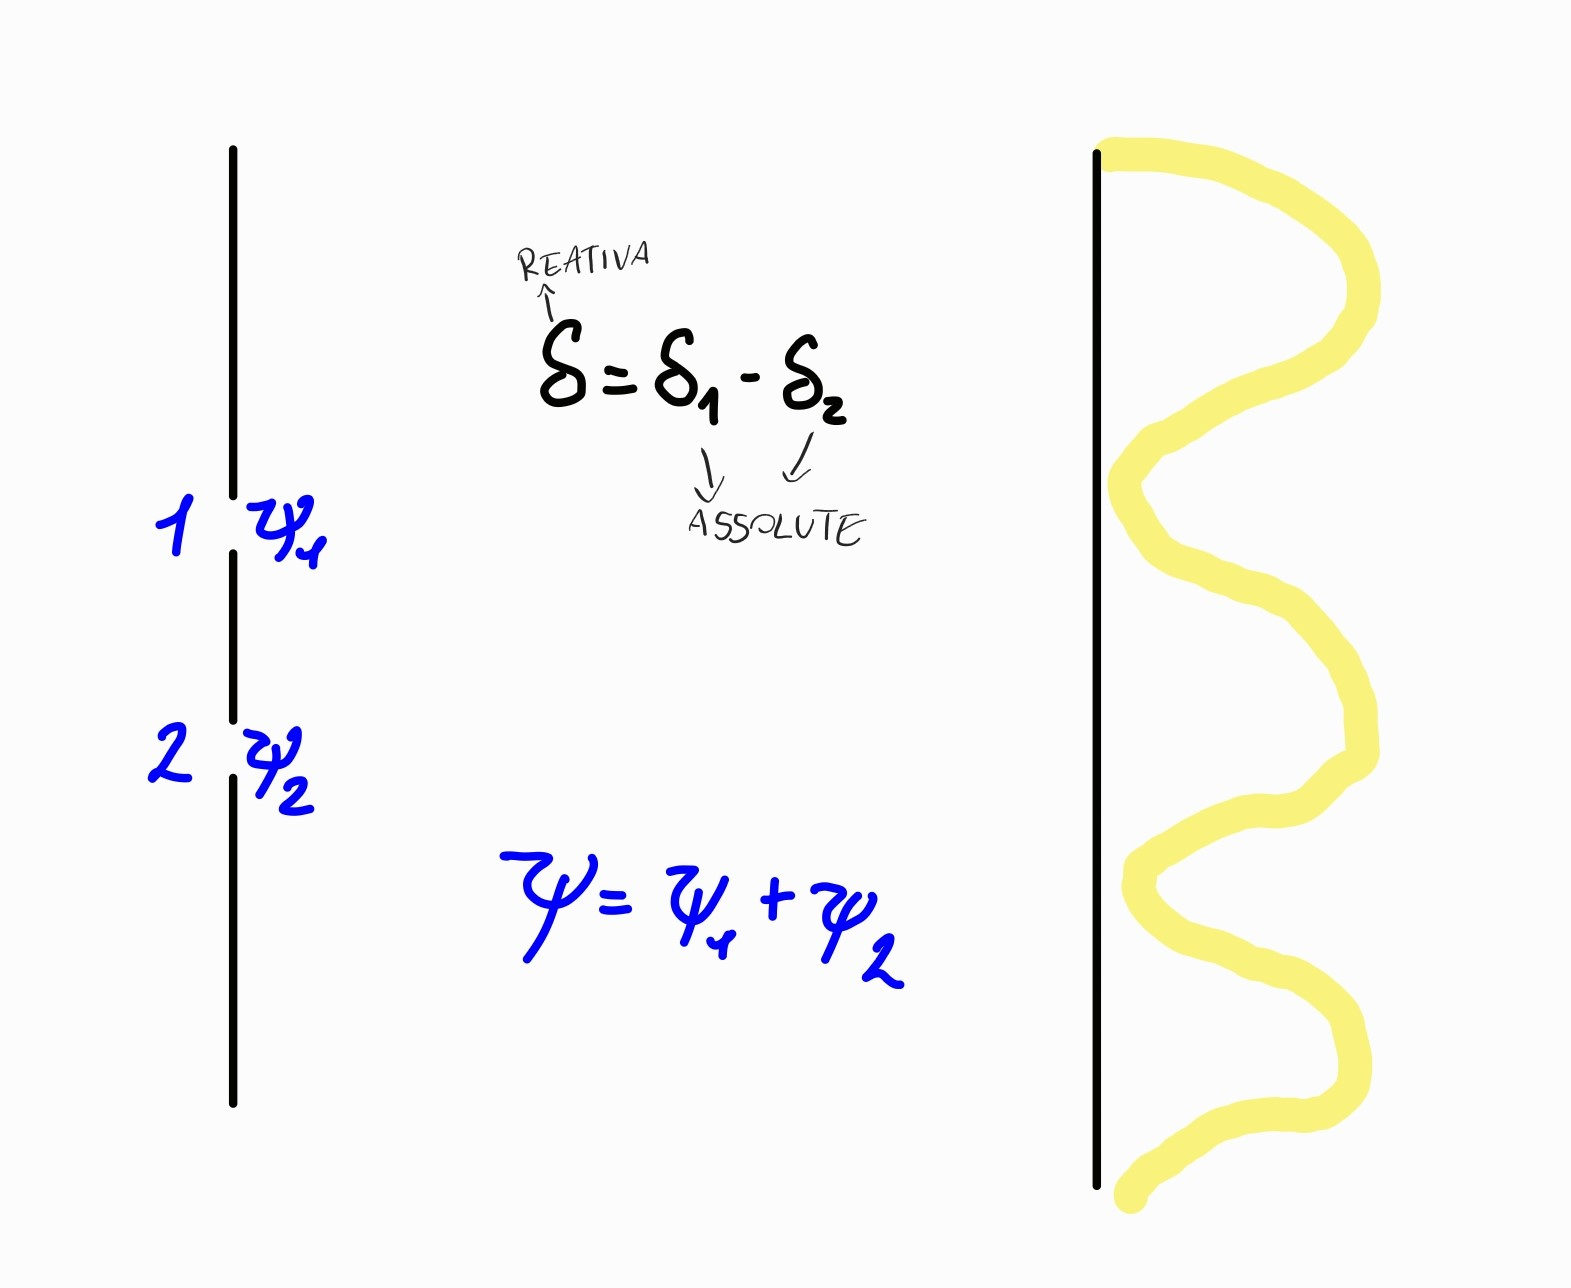
\includegraphics[width=0.31\textwidth]{Immagini/Doppia_fenditura.jpg}
    \caption{Esperimento della doppia fenditura.}
    \label{fig:fenditura}
\end{figure}
Quindi non è possibile misurare $\delta_1$ o $\delta_2$, ma solamente $\delta=\delta_1-\delta_2$. Inoltre, applicando delle trasformazioni del tipo $\delta_1\xrightarrow{}\delta_1+\alpha$ e $\delta_2\xrightarrow{}\delta_2+\alpha$ (con $\alpha$ una costante), la fase relativa $\delta$ rimane invariata. Trasformazioni di questo tipo sono dette \textit{trasformazioni globali di fase}\footnote{Il termine globale significa che la ridefinizione della fase è la stessa per tutti i punti dello spaziotempo.}, sotto queste trasformazioni la funzione d'onda varia in modo semplice:
\begin{equation}
    \psi\xrightarrow{}e^{i\alpha}\psi
\end{equation}
e la meccanica quantistica è invariante per questo tipo di trasformazioni. Infatti, se consideriamo il valor medio di un'osservabile generico , questo è indipendente dalla fase scelta:
\begin{equation}
    <\hat{O}>=\int\psi^*\hat{O}\psi d^3x
\end{equation}
Il gruppo che formano queste trasformazioni è detto $U(1)$. Possiamo, quindi, dire che la meccanica quantistica ha una simmetria di tipo $U(1)$ globale.

Ora, ci chiediamo cosa succede per trasformazioni $U(1)$ locali\footnote{Il termine locale indica semplicemente che la ridefinizione di fase varia, potenzialmente, punto per punto.}, ovvero trasformazioni del tipo:
\begin{equation}
    \psi\xrightarrow{}e^{i\alpha(t,\Vec{x})}\psi
\end{equation}
questo tipo di trasformazioni non sono simmetrie per nessuna teoria che descrive particelle libere, per esempio la \eqref{eq:eq_sch_part_lib}. Tuttavia, noi vogliamo forzare questo tipo di simmetria, per farlo è necessario modificare le teorie. Se, per esempio, prendiamo l'equazione \eqref{eq:eq_sch_part_car}, che descrive una particella carica sottoposta ad un campo elettromagnetico, abbiamo visto, nella sottosezione precedente, che vale una simmetria $U(1)$ locale, poiché $\chi(t,\Vec{x})$ dipende dalle coordinate spaziotemporali. Eppure, il costo da pagare è non banale. Infatti, affinché la teoria avesse la simmetria di gauge\footnote{Che è a tutti gli effetti una trasformazione $U(1)$ locale.}, è stato necessario introdurre nella teoria i campi $\Vec{A}$ e $\Phi$ e le rispettive trasformazioni di gauge. Quindi, possiamo dire, che le interazioni vengono dedotte imponendo delle simmetrie locali. L'idea è, dunque, di introdurre un'interazione a partire da una richiesta di simmetria locale. Tale procedura è quella usata per derivare tutte le interazioni fondamentali, ad esclusione di quella gravitazionale.

Possiamo riassumere quanto detto con il seguente enunciato del \textit{principio di gauge}: sia data una teoria che ha una simmetria globale rispetto ad un gruppo di Lie con $n$ generatori, si vuole imporre che la simmetria diventi locale, per farlo è necessario aggiungere alla teoria $n$ nuovi campi, i quali rappresentano nuove interazioni.

Ora applichiamolo ad un esempio di teoria di campo visto in precedenza.

Considerando un campo $\phi$ scalare complesso, possiamo definire la lagrangiana di Klein-Gordon:
\begin{equation}
  \mathcal{L}_{KG}=\partial_\mu\phi^*\partial^\mu\phi-\mu^2\phi^*\phi
\end{equation}
Otteniamo le equazioni di Eulero-Lagrange:
\begin{equation}
  (\Box+\mu^2)\phi^*=0 \qquad (\Box+\mu^2)\phi=0 
\end{equation}
tali equazioni lineari descrivono due particelle diverse di spin pari a zero e con la stessa massa, infatti questa formulazione viene usata per descrivere una particella e l'antiparticella corrispondente.

Sappiamo che, oltre alla simmetria per il gruppo di Poincaré, questa lagrangiana ha anche una simmetria interna per le trasformazioni:
\begin{equation}
\begin{gathered}
    \phi(x^\mu)\xrightarrow[\text{}]{\text{}}e^{i\alpha}\phi(x^\mu)\\
    \phi^*(x^\mu)\xrightarrow[\text{}]{\text{}}e^{-i\alpha}\phi^*(x^\mu)\\
    \partial_\mu \phi(x^\mu)\xrightarrow[\text{}]{\text{}}e^{i\alpha}\partial_\mu\phi(x^\mu)\\
   \partial_\mu \phi^*(x^\mu)\xrightarrow[\text{}]{\text{}}e^{-i\alpha}\partial_\mu\phi^*(x^\mu)\\
\end{gathered}
\end{equation}
ove $\alpha$ è una costante, tale simmetria porta con se la conservazione della carica. La simmetria in questione, per quanto detto precedentemente, è del tipo $U(1)$ globale. Le equazioni di Klein-Gordon descrivono particelle libere, tuttavia fisicamente viene da domandarsi per quale ragione particelle cariche non interagiscano. Per far emergere l'interazione dobbiamo usare il principio di gauge.

Quindi imponiamo che la simmetria da globale diventi locale, le trasformazioni per cui deve esserci simmetria, allora sono del tipo:
\begin{equation}
\begin{gathered}
    \phi(x^\mu)\xrightarrow[\text{}]{\text{}} \phi'(x^\mu)=e^{i\alpha(x^\mu)}\phi(x^\mu)\\
    \phi^*(x^\mu)\xrightarrow[\text{}]{\text{}}\phi'^*(x^\mu)=e^{-i\alpha(x^\mu)}\phi^*(x^\mu)\\
    \partial_\mu \phi(x^\mu)\xrightarrow[\text{}]{\text{}}\partial_\mu \phi'(x^\mu)=\partial_\mu[e^{i\alpha(x^\mu)}\phi(x^\mu)]\\
   \partial_\mu \phi^*(x^\mu)\xrightarrow[\text{}]{\text{}} \partial_\mu \phi'^*(x^\mu)=\partial_\mu[e^{-i\alpha(x^\mu)}\phi^*(x^\mu)]\\
\end{gathered}
\end{equation}
sviluppando i termini di derivata, otteniamo:
\begin{equation}
\begin{gathered}
    \partial_\mu \phi'(x^\mu)=\partial_\mu[e^{i\alpha(x^\mu)}\phi(x^\mu)]=e^{i\alpha(x^\mu)}[\partial_\mu\phi(x^\mu)]+i[\partial_\mu\alpha(x^\mu)]e^{i\alpha(x^\mu)}\phi(x^\mu)\\
  \partial_\mu \phi'^*(x^\mu)=\partial_\mu[e^{-i\alpha(x^\mu)}\phi^*(x^\mu)]=e^{-i\alpha(x^\mu)}[\partial_\mu\phi^*(x^\mu)]-i[\partial_\mu\alpha(x^\mu)]e^{-i\alpha(x^\mu)}\phi^*(x^\mu)\\
\end{gathered}
\end{equation}
il termine cinetico è dato dal prodotto tra i due:
\begin{equation}
\begin{aligned}
      \partial_\mu \phi'\partial^\mu \phi'^*&= \partial_\mu \phi\partial^\mu \phi^*-i\phi^*(\partial_\mu\phi)\partial^\mu\alpha+i\phi(\partial^\mu\phi^*)\partial_\mu\alpha+\partial_\mu\alpha\partial^\mu\alpha\phi^*\phi\\
      &=\partial_\mu \phi\partial^\mu \phi^*+i(\phi\partial_\mu\phi^*-\phi^*\partial_\mu\phi)\partial^\mu\alpha+\partial_\mu\alpha\partial^\mu\alpha\phi^*\phi
\end{aligned}
\end{equation}
il termine di massa è dato da:
\begin{equation}
\mu^2\phi'^*\phi'=\mu^2\phi^*\phi
\end{equation}

Concludiamo che a seguito di una trasformazione $U(1)$ locale, il termine di massa della lagrangiana va in se stesso, al contrario del termine cinetico, otteniamo, quindi, che la trasformazione proposta non è una simmetria per la lagrangiana di Klein-Gordon. Per forzare la simmetria modifichiamo la teoria, e dunque la lagrangiana, sostituendo la quadridivergenza con la derivata di gauge covariante\footnote{Questa, per definizione, deve trasformarsi come il campo, si usa dire che deve trasformasi vettorialmente.}. Le trasformazioni locali diventano\footnote{A queste trasformazioni abbiamo aggiunto un termine $e$ all'esponenziale, questo ci serve più avanti, comunque essendo una costante siamo liberi di farlo senza intaccare quanto detto sulle simmetrie $U(1)$ locali.}, quindi:
\begin{equation}
\begin{gathered}
    \phi(x^\mu)\xrightarrow[\text{}]{\text{}} \phi'(x^\mu)=e^{ie\alpha(x^\mu)}\phi(x^\mu)\\
    \phi^*(x^\mu)\xrightarrow[\text{}]{\text{}}\phi'^*(x^\mu)=e^{-ie\alpha(x^\mu)}\phi^*(x^\mu)\\
    D_\mu \phi(x^\mu)\xrightarrow[\text{}]{\text{}}D'_\mu \phi'(x^\mu)=e^{ie\alpha(x^\mu)}D_\mu\phi(x^\mu)\\
   D^*_\mu \phi^*(x^\mu)\xrightarrow[\text{}]{\text{}} D'^*_\mu \phi'^*(x^\mu)=e^{-ie\alpha(x^\mu)}D^*_\mu\phi^*(x^\mu)\\
\end{gathered}
\end{equation}
ove, ricordiamo, la derivata di gauge è definita come $D_\mu=\partial_\mu+iqA_\mu$, con $A_\mu$ detto campo di gauge\footnote{Il numero di campi di gauge da introdurre, affinché si possa imporre una simmetria, deve essere pari al numero di generatori del gruppo di cui si richiede la simmetria. In questo caso $U(1)$ ha un solo generatore e quindi il campo introdotto è uno solo; se la simmetria fosse stata imposta per il gruppo $SU(2)$, allora i campi da introdurre sarebbero stati tre, poiché i generatori del gruppo sono tre.}. D'ora in poi considereremo $q=-e$, quindi la derivata di gauge sarà $D_\mu=\partial_\mu-ieA_\mu$. Studiamo i nuovi termini di derivazione:
\begin{equation}
\begin{gathered}
    D'_\mu \phi'=[\partial_\mu-ieA'_\mu](e^{ie\alpha}\phi)=e^{ie\alpha}D_\mu\phi=e^{ie\alpha}[\partial_\mu-ieA_\mu]\phi\\
  e^{ie\alpha}(\partial_\mu\phi+ie\phi\partial_\mu\alpha-ieA'_\mu\phi)=e^{ie\alpha}[\partial_\mu\phi-ieA_\mu\phi]\\
  +ie\phi\partial_\mu\alpha-ieA'_\mu\phi=-ieA_\mu\phi\\
  A'_\mu=A_\mu+\partial_\mu\alpha
\end{gathered}
\end{equation}
Imponendo come si deve trasformare la derivata di gauge, abbiamo trovato come si trasforma il campo di gauge ad essa associato, lo stesso procedimento lo si può fare anche con il campo complesso coniugato $\phi^*$.

Alla luce di questo, scrivere una lagrangiana che abbia una simmetria $U(1)$ locale, diventa banale:
\begin{equation}
  \mathcal{L}=D_\mu\phi(D^\mu\phi)^*-\mu^2\phi^*\phi=(\partial_\mu-ieA_\mu)\phi(\partial^\mu+ieA^\mu)\phi^*-\mu^2\phi^*\phi
\end{equation}
tuttavia neanche questa teoria è completa, perché manca il termine cinetico di $A_\mu$, ossia $\partial_\nu A_\mu$, il quale ne descrive la dinamica. Quindi dobbiamo aggiungere un termine alla lagrangiana, ovviamente tale termine dovrà rispettare tutti i requisiti necessari al fine che la lagrangiana soddisfi tutte le proprietà richieste (gauge invarianza e simmetria gruppo di Poincaré).
\begin{equation}
  \mathcal{L}_{QED}=(\partial_\mu-ieA_\mu)\phi(\partial^\mu+ieA^\mu)\phi^*-\mu^2\phi^*\phi-\dfrac{1}{16\pi}F_{\mu\nu}F^{\mu\nu}
\end{equation}
questa è detta \textit{lagrangiana dell'elettrodinamica scalare}.

Sviluppando i termini si ottiene:
\begin{equation}
\begin{aligned}
     \mathcal{L}_{QED}&=\partial_\mu\phi\partial^\mu\phi^*-\mu^2\phi^*\phi+ieA^\mu(\phi^*\partial_\mu\phi-\phi\partial_\mu\phi^*)+e^2A_\mu A^\mu\phi^*\phi-\dfrac{1}{16\pi}F_{\mu\nu}F^{\mu\nu}\\
     &=\mathcal{L}_{KG}+\mathcal{L}_{INT}+\mathcal{L}_{M}
\end{aligned}
\end{equation}
Possiamo notare che i primi due termini sono la lagrangiana di Klein-Gordon (per particelle libere), i termini terzo, quarto e quinto sono la lagrangiana che descrive le interazioni (poiché hanno dipendenze dai campi superiori a due), infine il sesto è la lagrangiana  di Maxwell per il campo di gauge. 

Ci rimane da calcolare le equazioni di Eulero-Lagrange, per i tre campi indipendenti $\phi$, $\phi^*$ e $A_\nu$. Partiamo da $\phi^*$:
\begin{equation}
\begin{gathered}
      \partial_\mu\dfrac{\partial \mathcal{L}_{QED}}{\partial(\partial_\mu \phi^*)}=\dfrac{\partial\mathcal{L}_{QED}}{\partial \phi^*} \\
      \partial_\mu(\partial^\mu\phi-ieA^\mu\phi)=-\mu^2\phi+ieA^\mu\partial_\mu\phi+e^2A_\mu A^\mu\phi\\
      \Box\phi+\mu^2\phi=ie\partial_\mu(A^\mu\phi)+ieA^\mu\partial_\mu\phi+e^2A_\mu A^\mu\phi
\end{gathered}
\end{equation}
in maniera del tutto analoga, l'equazione per $\phi$ si determina semplicemente sostituendo con il complesso coniugato:
\begin{equation}
      \Box\phi^*+\mu^2\phi^*=ie\partial_\mu(A^\mu\phi^*)+ieA^\mu\partial_\mu\phi^*+e^2A_\mu A^\mu\phi^*
\end{equation}
Infine, rimane solamente $A_\nu$:
\begin{equation}
\begin{gathered}
    \partial_\mu\dfrac{\partial \mathcal{L}_{QED}}{\partial(\partial_\mu A_\nu)}=\dfrac{\partial\mathcal{L}_{QED}}{\partial A_\nu}\\
    \partial\left(-\dfrac{F^{\mu\nu}}{4\pi}\right)=ie(\phi^*\partial^\nu\phi-\phi\partial^\nu\phi^*)+2A^\nu\phi\phi^*\\
    \partial_\mu F^{\mu\nu}=4\pi[ie(\phi\partial^\nu\phi^*-\phi^*\partial^\nu\phi)-2A^\nu\phi\phi^*]
\end{gathered}
\end{equation}
Quindi è un sistema di tre campi accoppiati tra loro, la cui dinamica è descritta da queste tre equazioni.

\subsection{Rottura spontanea di simmetria}
Lo studio effettuato nella sezione precedente è valido solo per interazioni i cui mediatori sono campi non massivi. Infatti, per rendere il campo massivo dovremmo aggiungere nella lagrangiana un termine di massa di Proca $(m^2A_\mu A^\mu)$, però come abbiamo già visto questo termine rompe la gauge invarianza della lagrangiana.

\`E possibile aggirare lostacolo mediante la così detta \textit{rottura spontanea di simmetria}. Questo concetto, prima che venisse usato nella teoria dei campi, era già noto nell'ambito della fisica della materia condensata. Un esempio ci è dato dal ferromagnetismo. In un ferromagnete ci sono vari domini di spin, sappiamo che sopra la temperatura di Curie i domini sono orientati isotropicamente, mentre sotto la temperatura di Curie gli spin si allineano dando origine ad una magnetizzazione netta.
\begin{figure}[H]
    \centering
    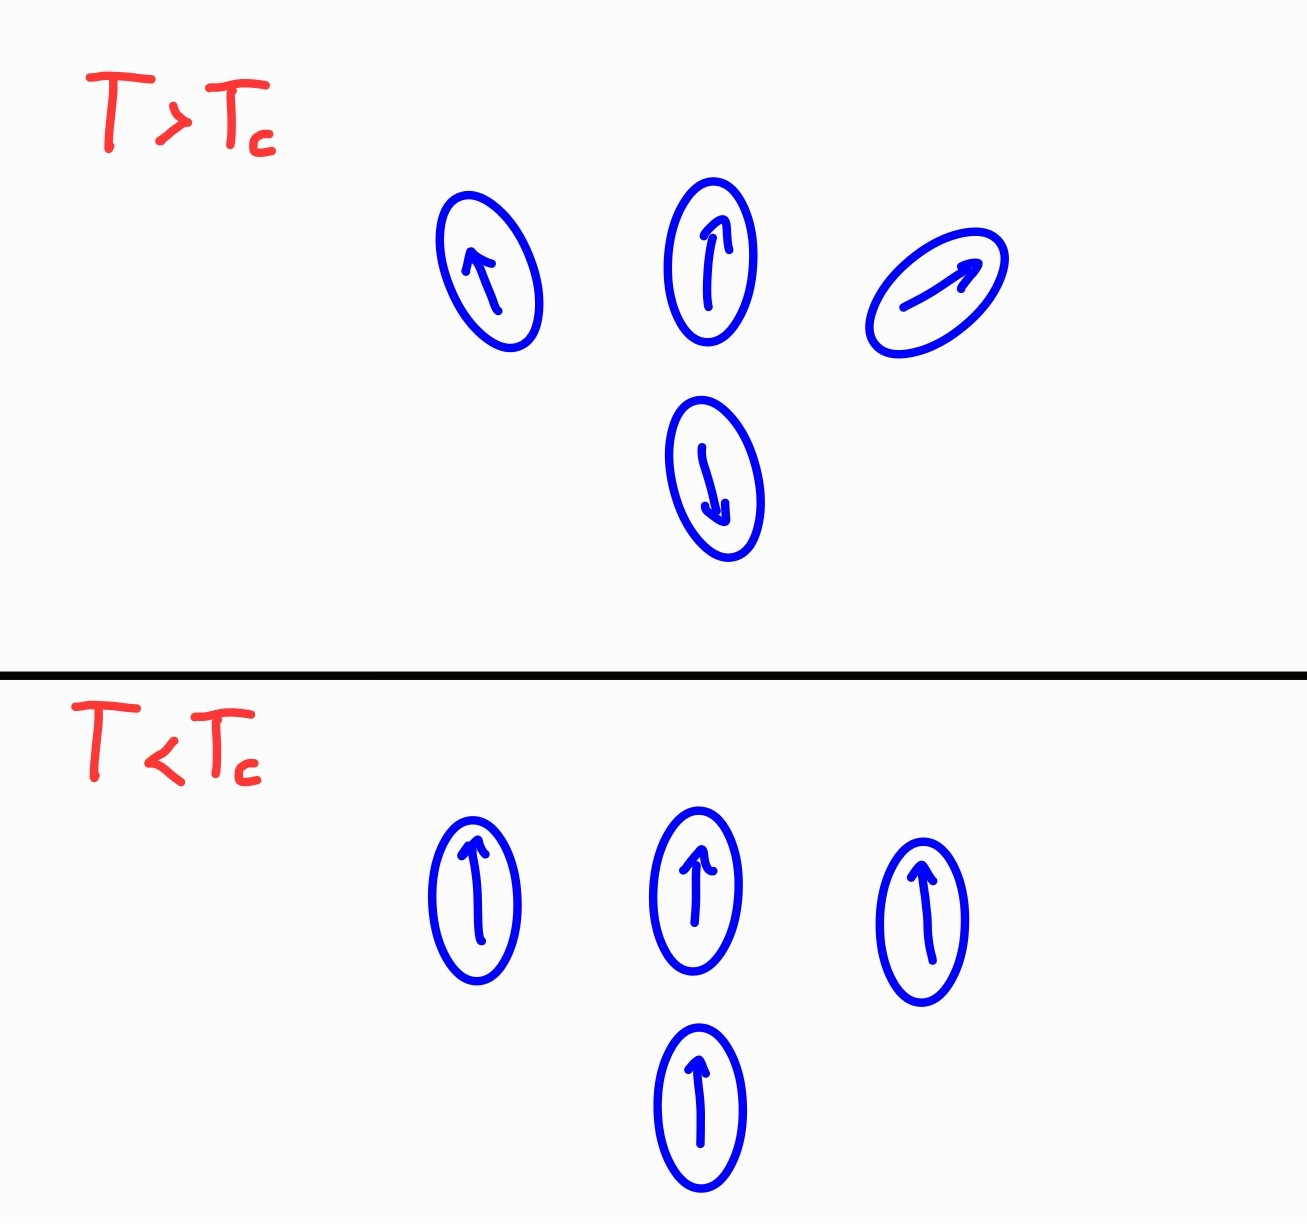
\includegraphics[width=0.31\textwidth]{Immagini/Spin.jpg}
    \caption{Spin di un ferromganete.}
    \label{fig:ferromagnete}
\end{figure}
L'Hamiltoniana associata è del tipo $H=-\sum_{i\neq j}\mu_{ij}\Vec{s}_i\cdot\Vec{s}_j$, questa risulta essere invariante per rotazioni. Tuttavia, nel caso $T<T_C$ il sistema o, meglio, lo stato fondamentale del sistema rompe l'invarianza per rotazioni.

Generalizzando il concetto, possiamo dire che: data una teoria con una certa simmetria, se lo stato fondamentale non rispetta tale simmetria, allora si parla di rottura spontanea di simmetria.

Analizziamo, ora, un esempio di teoria di campo visto in precedenza.

Consideriamo un campo scalare reale con una lagrangiana del tipo:
\begin{equation}\phantomsection\label{eq:lag}
  \mathcal{L}(\phi,\partial_\mu\phi)=\partial_\mu\phi\partial^\mu\phi-V(\phi)
\end{equation}
dall'equazione di Eulero-Lagrange
\begin{equation}
    \partial_\mu\dfrac{\partial \mathcal{L}}{\partial(\partial_\mu\phi)}-\dfrac{\partial\mathcal{L}}{\partial \phi}=0
\end{equation}
otteniamo l'equazione del moto:
\begin{equation}
   \Box \phi+\dfrac{dV}{d\phi}=0
\end{equation}
In generale, per teorie di questo tipo abbiamo che il momento coniugato è
\begin{equation}
    \mathcal{P}=\dfrac{\partial\mathcal{L}}{\partial \Dot{\phi}}=\Dot{\phi} \quad \text{ove }\quad\dot{\phi}=\dfrac{\partial \phi}{\partial t}
\end{equation}
Quindi possiamo definire una Hamiltoniana:
\begin{equation}
    H=\int d^3x\mathcal{H}
\end{equation}
ove la densità di Hamiltoniana è definita come:
\begin{equation}
    \mathcal{H}=\mathcal{P}\dot{\phi}-\mathcal{L}=\dfrac{\dot{\phi}^2}{2}+\left(\Vec{\nabla}\phi\right)^2+V(\phi)
\end{equation}
Ora, ci chiediamo quale sia la configurazione di campo che minimizzi l'Hamiltoniana. Osservando la forma analitica vediamo che l'Hamiltoniana sarà minima per $\phi$ constante (così che i primi due termini siano nulli) e il $\phi$ che minimizza il potenziale $V(\phi)$.

 Consideriamo il seguente potenziale
 \begin{equation}\phantomsection\label{eq:pot_1}
    V(\phi)=\dfrac{1}{2}m^2\phi^2+\dfrac{1}{4}\lambda\phi^4
\end{equation}
ove richiediamo che $\lambda>0$, altrimenti $ V(\phi)\xrightarrow{\phi\xrightarrow{}\infty}-\infty$, per cui non avremo alcun punto di minimo globale sul quale fissare lo stato fondamentale. Studiando il potenziale troviamo che ha forma:
\begin{figure}[H]
    \centering
    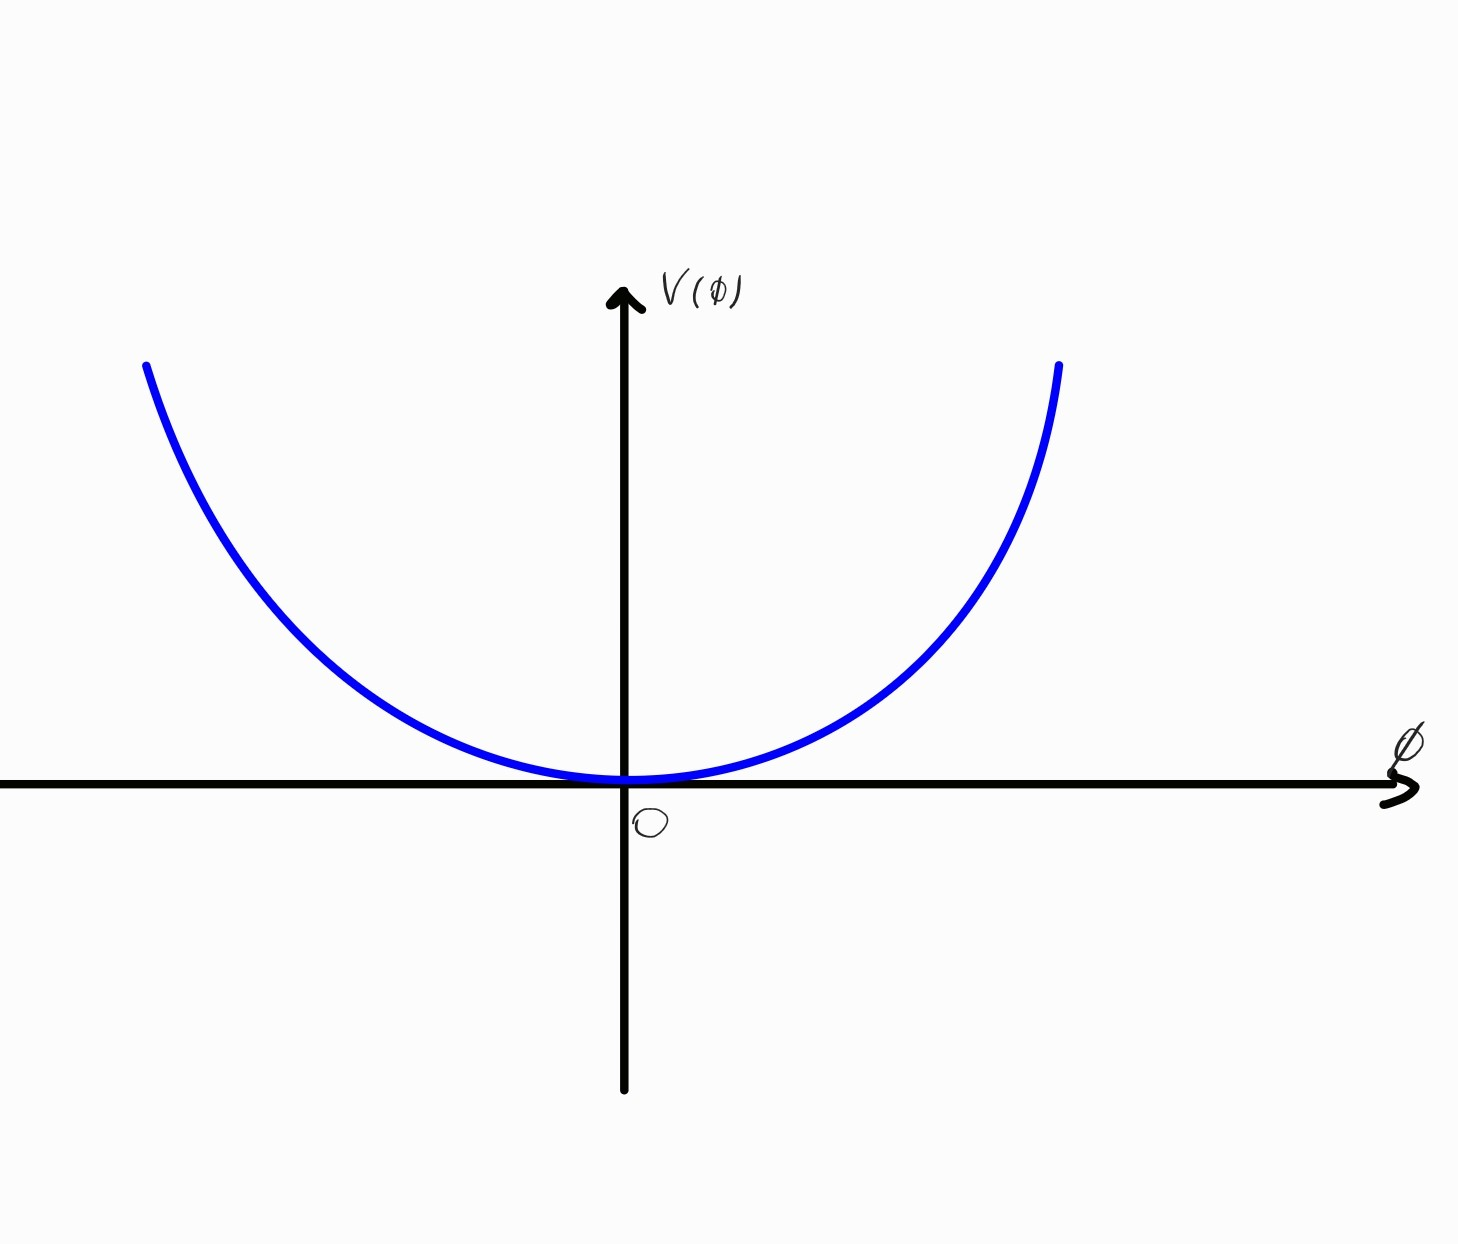
\includegraphics[width=0.31\textwidth]{Immagini/Pot1.jpg}
    \caption{Potenziale $ V(\phi)=\dfrac{1}{2}m^2\phi^2+\dfrac{1}{4}\lambda\phi^4$.}
    \label{fig:pot1}
\end{figure}
per cui fissiamo lo stato fondamentale nel punto $\phi=0$.

Osserviamo che la lagrangiana \eqref{eq:lag} con potenziale \eqref{eq:pot_1} ha una simmetria per la trasformazione discreta di parità $\phi\xrightarrow{}-\phi$, inoltre notiamo che a seguito di una tale trasformazione lo stato fondamentale rimane invariato; in tal caso si parla di \textit{simmetria ordinaria}.

Dall'equazione di Eulero-Lagrange otteniamo:
\begin{equation}
    (\Box+m^2)\phi=-\lambda\phi^3
\end{equation}
che descrive particelle massive di spin nullo, il temine cubico rappresenta l'autointerazione del campo.

 Consideriamo un altro potenziale
 \begin{equation}\phantomsection\label{eq:pot_2}
    V(\phi)=-\dfrac{1}{2}\mu^2\phi^2+\dfrac{1}{4}\lambda\phi^4
\end{equation}
sempre con $\lambda>0$ e c'è la simmetria per $\phi\xrightarrow{}-\phi$. Possiamo, inoltre, osservare che, apparentemente, la massa sia immaginaria, d'altronde l'equazione di campo assume la forma:
\begin{equation}
    (\Box-\mu^2)\phi=-\lambda\phi^3
\end{equation}

Derivando il potenziale troviamo:
 \begin{equation}
    \dfrac{\partial V(\phi)}{\partial \phi}=-\mu^2\phi+\lambda\phi^3
\end{equation}
da cui i punti critici sono per:
\begin{equation}
   \phi=0 \quad\land\quad\phi=\pm\sqrt{\dfrac{\mu^2}{\lambda}}=\pm v
\end{equation}
graficandola:
\begin{figure}[H]
    \centering
    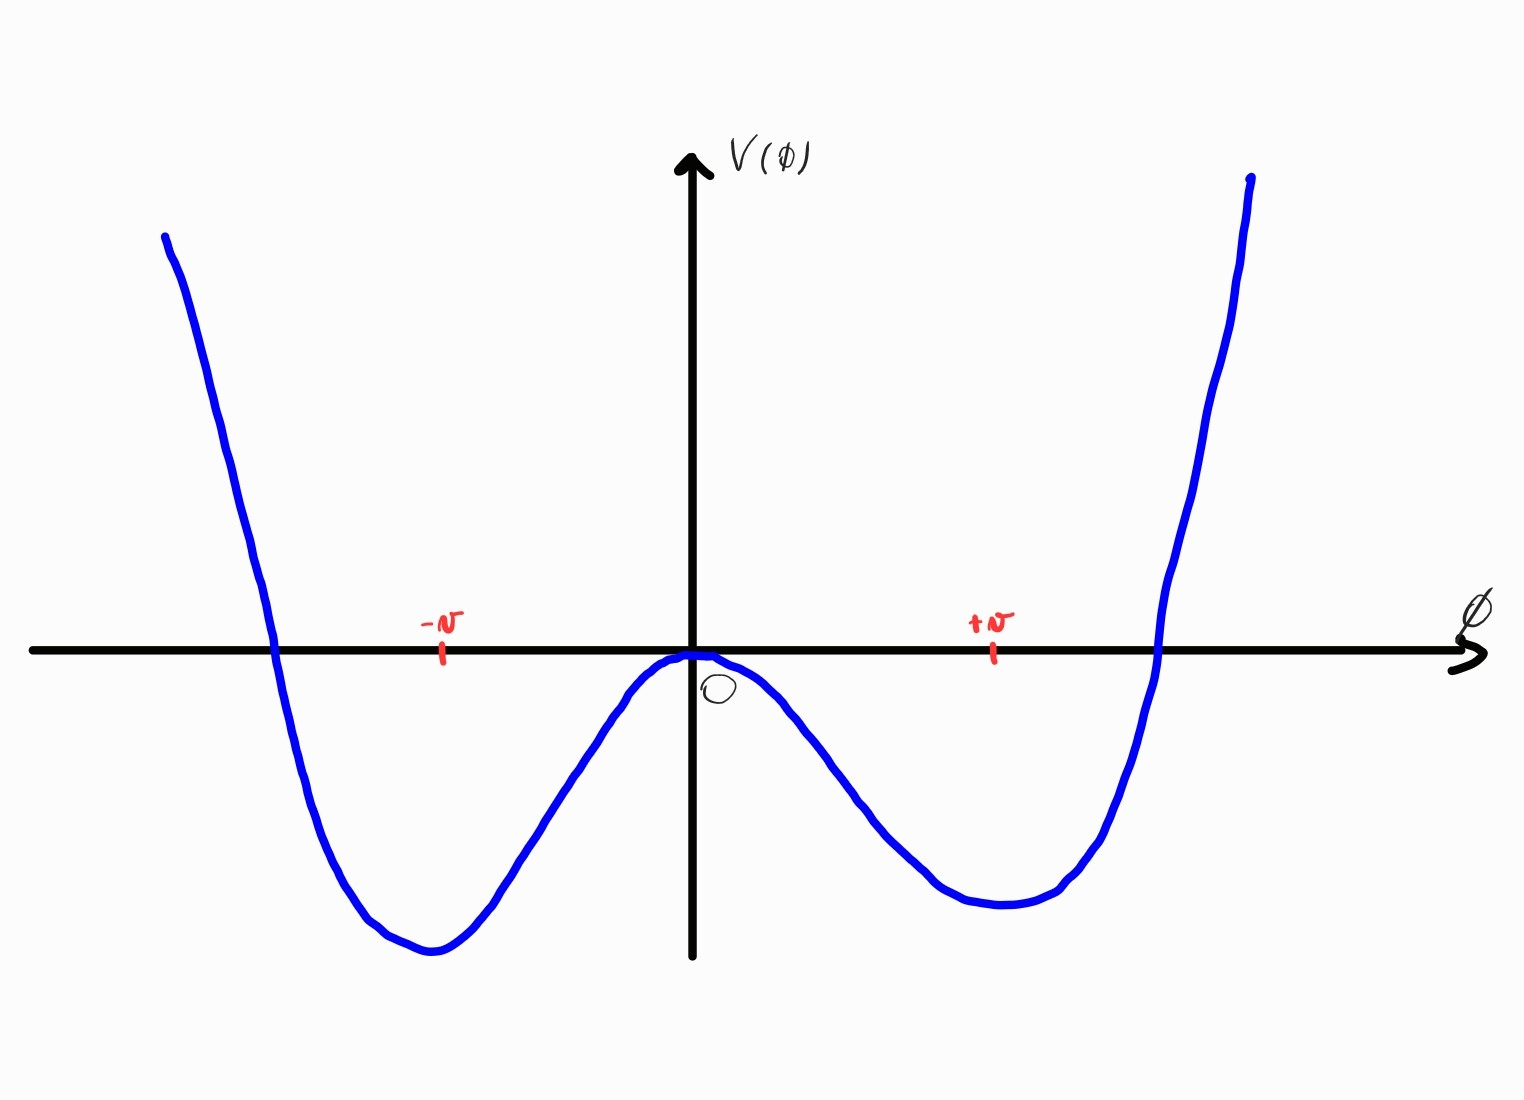
\includegraphics[width=0.31\textwidth]{Immagini/Pot2.jpg}
    \caption{Potenziale $ V(\phi)=-\dfrac{1}{2}\mu^2\phi^2+\dfrac{1}{4}\lambda\phi^4$.}
    \label{fig:pot2}
\end{figure}
ci accorgiamo che il punto $\phi=0$ è di massimo locale e dunque, essendo instabile, non può essere lo stato fondamentale. Scegliamo come stato fondamentale $\phi=v$, ci accorgiamo che applicando una trasformazione di parità lo stato fondamentale non rimane lo stesso, ecco che si verifica la rottura spontanea di simmetria.
Inoltre, la questione della massa immaginaria si risolve autonomamente, infatti per dire che la massa era immaginaria bisognava implicitamente assumere come stato fondamentale $\phi=0$, ma questo non lo è.

 Vogliamo studiare le fluttuazioni del campo rispetto allo stato fondamentale, per farlo definiamo un nuovo campo:
 \begin{equation}
     \phi'(x)=\phi-v
 \end{equation}
questo mi parametrizza le oscillazioni attorno allo stato fondamentale. Riscriviamo la lagrangiana in termini del nuovo campo:
\begin{equation}\phantomsection\label{eq:lag_phi'}
  \mathcal{L}=\partial_\mu\phi'\partial^\mu\phi'-V(\phi')
\end{equation}
il potenziale sarà:
\begin{equation}
\begin{aligned}
      V(\phi')&=-\dfrac{1}{2}\mu^2(\phi'+v)^2+\dfrac{1}{4}\lambda(\phi'+v)^4\\
      &=-\dfrac{\mu^2}{2}(\phi'^2+2\phi' v+v^2)+\dfrac{\lambda}{4}(\phi'^4+4\phi'^3v+6\phi'^2v^2+4\phi' v^3+v^4)
\end{aligned}
\end{equation}
 studiamo ogni termine in funzione dell'ordine di $\phi'$:
 \begin{equation}
\begin{aligned}
 &\phi'^0:      \quad  -\dfrac{\mu^2}{2}v^2+\dfrac{\lambda}{4} v^4\\
  &\phi':      \quad   -\mu^2v+\lambda v^3=   v(-\mu^2+\lambda v^2)=0                                        \\
 & \phi'^2:     \quad -\dfrac{\mu^2}{2}+\dfrac{3}{2}\lambda v^2=\mu^2                                              \\
 & \phi'^3:  \quad             \lambda v                                             \\
 & \phi'^4:\quad       \dfrac{\lambda}{4}
\end{aligned}\footnote{Come avevamo già capito il termine di massa non ha massa immaginaria una volta fissato il giusto stato fondamentale.}
\end{equation}
Il potenziale assume, quindi, la forma:
\begin{equation}\phantomsection\label{eq:pot_phi'}
      V(\phi')=-\mu^2 \phi'^2+\mu^2\left[\dfrac{1}{v}\phi'^3+\dfrac{1}{4v^2}\phi'^4-\dfrac{\mu^2}{4\lambda}\right]
\end{equation}
l'equazione di Eulero-Lagrange è:
\begin{equation}
    (\Box+2\mu^2)\phi'=-\dfrac{3\mu^2}{v}\phi'^2-\dfrac{\mu^2}{v^2}\phi'^4
\end{equation}
 se chiamiamo $m^2=2\mu^2\xrightarrow{}m=\sqrt{2}\mu$, abbiamo trovato che la massa è reale.

 Anche per la lagrangiana \eqref{eq:lag_phi'} con il potenziale \eqref{eq:pot_phi'} vale la simmetria per la trasformazione di parità $\phi\xrightarrow{}-\phi$, anche se non è manifesta.



Nei due casi appena esaminati avevamo che la simmetria era di tipologia discreta, ora vogliamo esaminare casi in cui la simmetria sia continua.




 Per farlo, consideriamo due campi scalari reali $\phi_1$ e $\phi_2$, con una lagrangiana del tipo:
\begin{equation}
  \mathcal{L}=\dfrac{1}{2}(\partial_\mu\phi_1\partial^\mu\phi_1+\partial_\mu\phi_2\partial^\mu\phi_2)-V(\phi_1^2+\phi_2^2)
\end{equation}
questa lagrangiana ha una simmetria continua di tipo $SO(2)$:

\begin{equation}
   \begin{pmatrix}
 \phi_1' \\
\phi_2'\\
\end{pmatrix}=\begin{pmatrix}
 \cos{\theta}&\sin{\theta}\\
-\sin{\theta} &\cos{\theta}\\
\end{pmatrix} \begin{pmatrix}
 \phi_1 \\
\phi_2\\
\end{pmatrix}
\end{equation}
Consideriamo un potenziale del tipo
\begin{equation}
    V(\phi_1^2+\phi_2^2)=\dfrac{m^2}{2}(\phi_1^2+\phi_2^2)+\dfrac{\lambda}{4}(\phi_1^2+\phi_2^2)^2
\end{equation}
determiniamo lo stato fondamentale, per farlo calcoliamo le derivate del potenziale:
\begin{equation}
    \begin{cases}
        \dfrac{\partial V}{\partial\phi_1}=m^2\phi_1+\lambda\phi_1(\phi_1^2+\phi_2^2)=0\\
        \\
        \dfrac{\partial V}{\partial\phi_2}=m^2\phi_2+\lambda\phi_2(\phi_1^2+\phi_2^2)=0
    \end{cases}
\end{equation}
risolvendo il sistema troviamo che la soluzione al sistema è $\phi_1=\phi_2=0$, questo è il nostro stato fondamentale.
La rappresentazione del potenziale è: 
\begin{figure}[H]
    \centering
    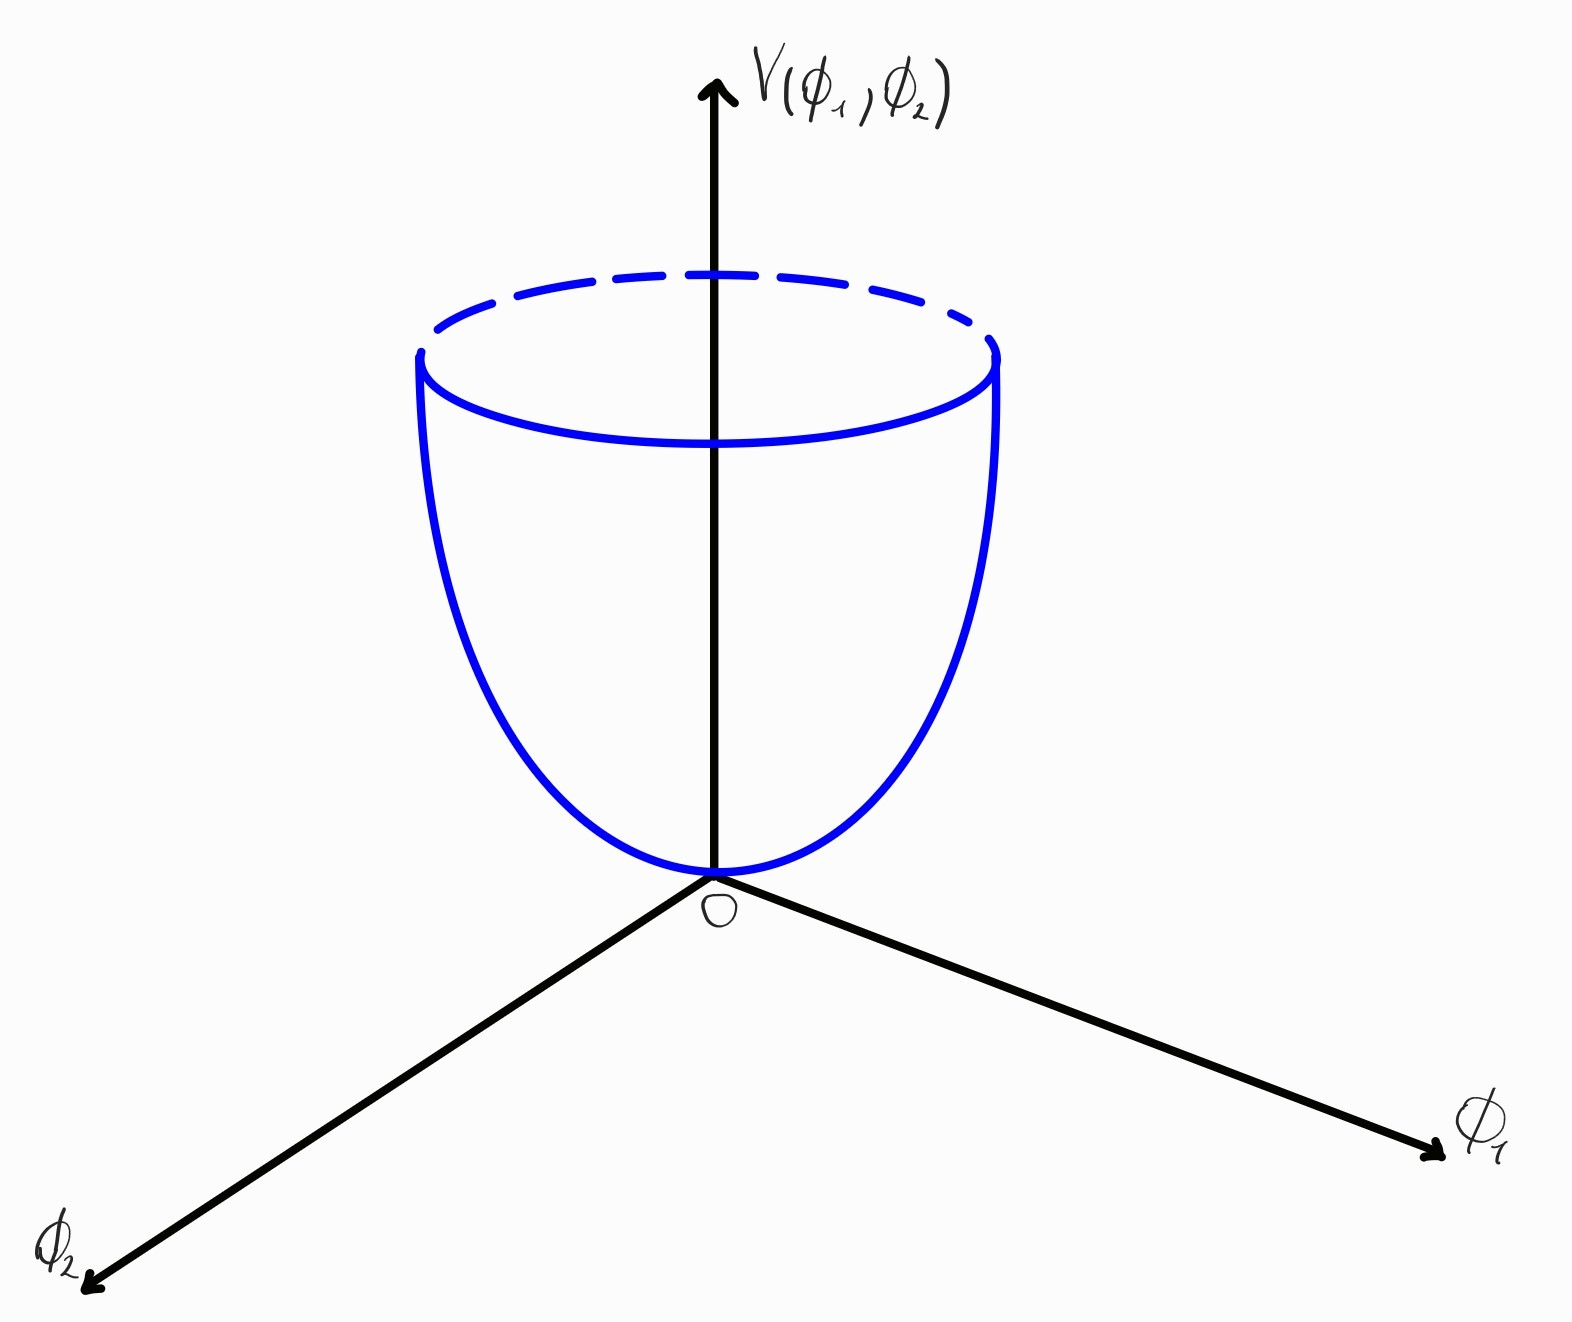
\includegraphics[width=0.31\textwidth]{Immagini/Pot3.jpg}
    \caption{Potenziale $ V(\phi_1^2+\phi_2^2)=\dfrac{m^2}{2}(\phi_1^2+\phi_2^2)+\dfrac{\lambda}{4}(\phi_1^2+\phi_2^2)^2$.}
    \label{fig:pot3}
\end{figure}
Per una rotazione nel piano dei campi lo stato fondamentale rimane fisso, quindi abbiamo una simmetria ordinaria.



Consideriamo un altro esempio, sempre a partire da due campi scalari reali $\phi_1$ e $\phi_2$, con un potenziale del tipo
\begin{equation}
    V(\phi_1^2+\phi_2^2)=-\dfrac{\mu^2}{2}(\phi_1^2+\phi_2^2)+\dfrac{\lambda}{4}(\phi_1^2+\phi_2^2)^2
\end{equation}
anche qui sembra esserci un massa immaginaria, tuttavia ormai abbiamo compreso non essere sempre così semplice.

Determiniamo lo stato fondamentale, le derivate del potenziale sono:
\begin{equation}
    \begin{cases}
        \dfrac{\partial V}{\partial\phi_1}=-\mu^2\phi_1+\lambda\phi_1(\phi_1^2+\phi_2^2)=0\\
        \\
        \dfrac{\partial V}{\partial\phi_2}=-\mu^2\phi_2+\lambda\phi_2(\phi_1^2+\phi_2^2)=0
    \end{cases}
\end{equation}
risolvendo il sistema troviamo che la soluzione si ha per $\phi_1=\phi_2=0$ e per $\phi_1^2+\phi_2^2=\dfrac{\mu^2}{\lambda}=v^2$, ove quest'ultima è una circonferenza.

La rappresentazione del potenziale è: 
\begin{figure}[H]
    \centering
    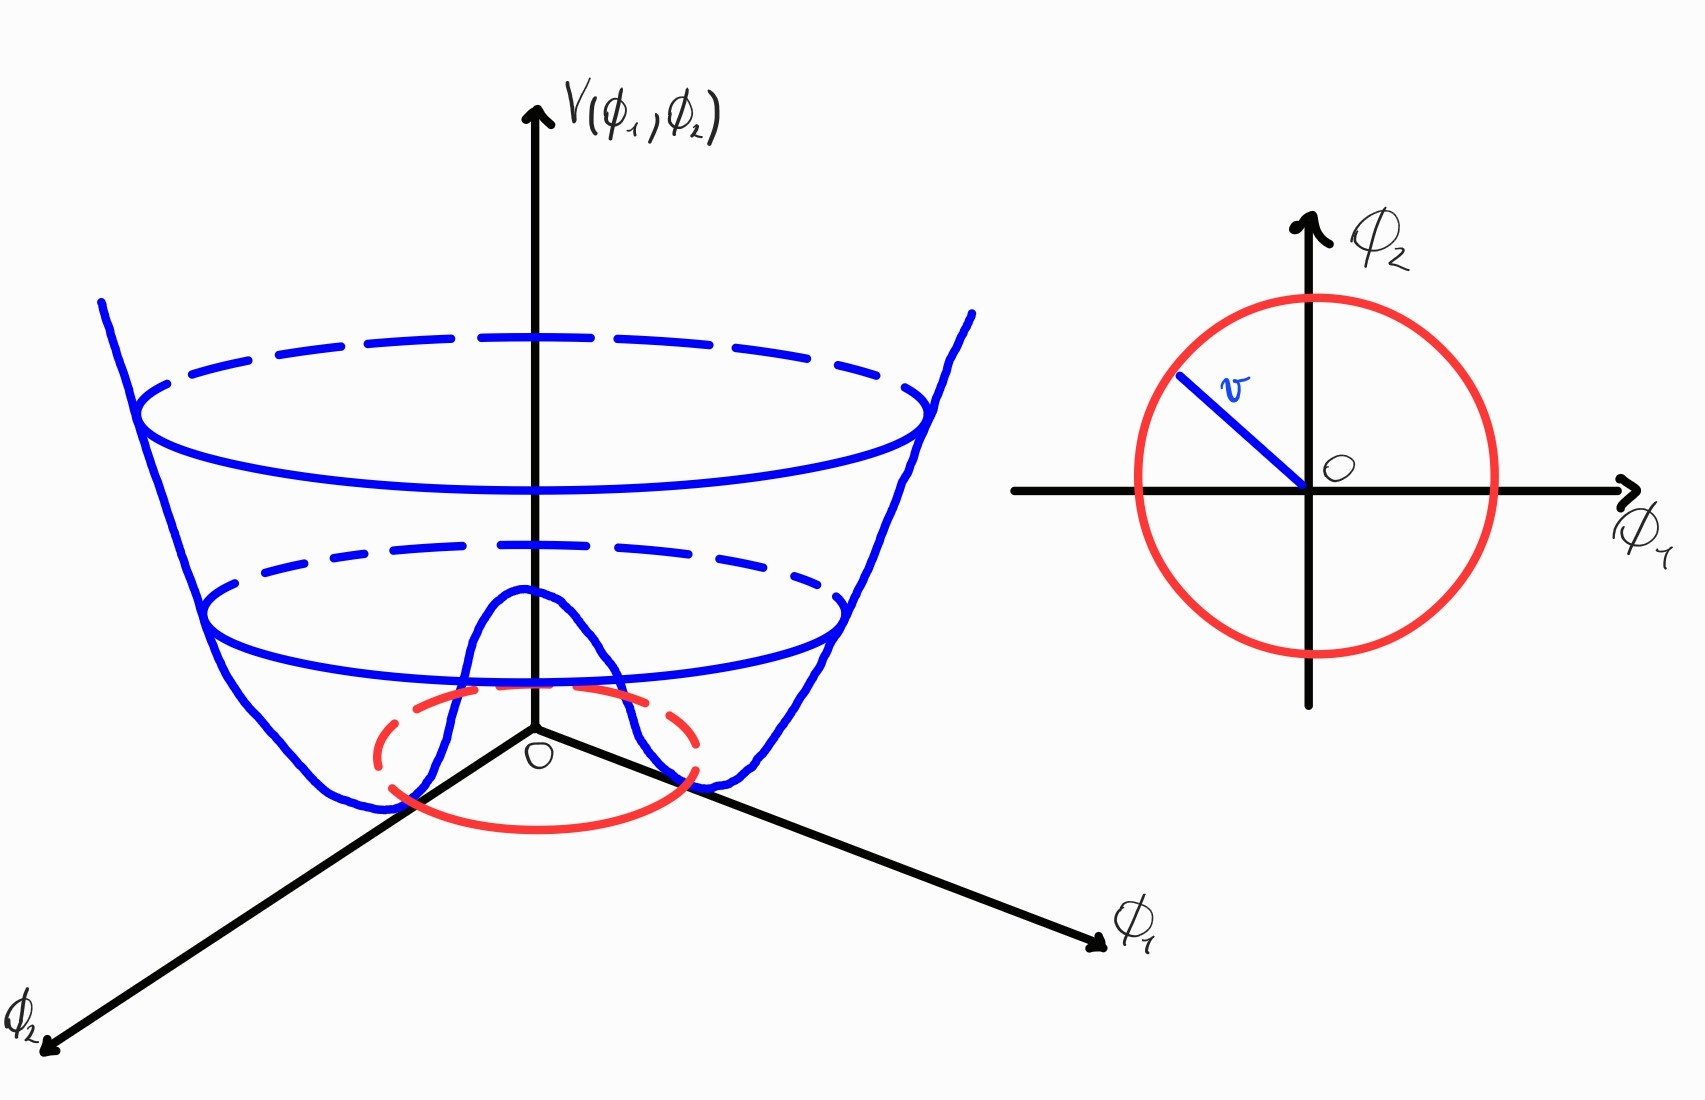
\includegraphics[width=0.31\textwidth]{Immagini/Pot4.jpg}
    \caption{Potenziale $  V(\phi_1^2+\phi_2^2)=-\dfrac{\mu^2}{2}(\phi_1^2+\phi_2^2)+\dfrac{\lambda}{4}(\phi_1^2+\phi_2^2)^2$.}
    \label{fig:pot4}
\end{figure}
Notiamo che il punto $\phi_1=\phi_2=0$ è un massimo e dunque non è lo stato fondamentale, al contrario dei punti corrispondenti alla circonferenza, possiamo, quindi, scegliere in maniera arbitraria un punto tra questi, per semplicità scegliamo $\phi_1=v$ e $\phi_2=0$.
Vogliamo capire che tipo di particelle rappresenta la teoria, per falo dobbiamo studiare le fluttuazioni del campo rispetto allo stato fondamentale, quindi definiamo
i nuovi campi:
\begin{equation}
 \eta=\phi'_1=\phi_1-v\qquad\xi=\phi'_2=\phi_2
\end{equation}
Per lo stato fondamentale non vi è la simmetria rispetto a $SO(2)$, quindi si ha la rottura spontanea di simmetria.

La lagrangiana riscritta in questi campi è:
\begin{equation}
  \mathcal{L}(\eta,\xi)=\dfrac{1}{2}\partial_\mu\eta\partial^\mu\eta+\dfrac{1}{2}\partial_\mu\xi\partial^\mu\xi-V(\eta,\xi)
\end{equation}
mentre il potenziale assume la forma
\begin{equation}
V(\eta,\xi)=-\dfrac{\mu^2}{2}[\eta^2+2\eta v+v^2+\xi^2]+\dfrac{\lambda}{4}[\eta^4+6\eta^2v^2+v^4+\xi^4+4\eta^3v+2\eta^2\xi^2+4\eta v^3+4v\eta\xi^2+2v^2\xi^2]
\end{equation}
 studiamo ogni termine in funzione dell'ordine di $\eta$ e $\xi$ (scriveremo solo i termini necessari a trarre le conclusioni):
 \begin{equation}
\begin{aligned}
 &\eta: \quad  -\mu^2 v+\lambda v^3=0\\  
 & \eta^2:     \quad -\dfrac{\mu^2}{2}+\dfrac{3}{2}\lambda v^2=\mu^2                                              \\
 & \xi:  \quad           0             \\
 & \xi^2:\quad      -\dfrac{\mu^2}{2}+\dfrac{1}{2}\lambda v^2=0\\
&\vdots
\end{aligned}
\end{equation}

Riscrivendo la lagrangiana abbiamo:
\begin{equation}
  \mathcal{L}(\eta,\xi)=\dfrac{1}{2}\partial_\mu\eta\partial^\mu\eta+\dfrac{1}{2}\partial_\mu\xi\partial^\mu\xi-\mu^2\eta^2+\cdots
\end{equation}
Quindi la teoria descrive una particella del campo $\eta$, che è massiva di massa $m=\sqrt{2}\mu$ reale, e una particella del campo $\xi$ non è massiva. La particella non massiva è chiamata \textit{bosone di Goldstone}.

Questo discende dal teorema di Goldstone il quale afferma che quando una simmetria continua viene spontaneamente rotta nello spettro di massa compaiono necessariamente delle particelle di massa nulla.



Ripercorriamo i punti fondamentali delle ultime pagine ed aggiungiamo alcune considerazioni.

La questione iniziale era che, considerando le teorie di gauge, a seguito del principio di gauge, queste comportavano l'introduzione dei campi di gauge non massivi, l'esempio che abbiamo visto era quello dell'elettrodinamica scalare. Tuttavia, noi vogliamo descrivere altri tipi di interazioni che hanno mediatori massivi, pur mantenendo le proprietà delle teorie di gauge. Il motivo per cui vogliamo mantenere queste proprietà risiede nel fatto che, quantisticamente, le teorie di gauge sono rinormalizzabili\footnote{Quindi è possibile attribuirgli un significato fisico.}. Con la rottura spontanea di simmetria, solo apparentemente, sembra di andare in direzione opposta al problema, poiché il teorema di Goldstone afferma l'esistenza di altri campi non massivi, cionondimeno avviene una sorta di miracolo quando si mette assieme la rottura spontanea di simmetria e le teorie di gauge. A livello di gradi di libertà, la differenza tra un campo vettoriale massivo e uno vettoriale non massimo è che il primo ha tre gradi di libertà (una direzione trasversale positiva, una direzione trasversale negativa e una longitudinale)\footnote{Lo abbiamo visto con la lagrangiana di Proca.}, il secondo solo due (una direzione trasversale positiva, una direzione trasversale negativa)\footnote{Lo abbiamo visto con la lagrangiana elettromagnetica}. Il miracolo che avviene sembra essere che, in qualche modo, il bosone di Goldstone venga fagocitato dal campo di gauge, donando, così, al campo di gauge massa e quindi tre possibili polarizzazioni. Nel processo di rottura della simmetria di gauge, la lagrangiana non perde tale simmetria proprio perché la rottura è spontanea; ciò che rompe la simmetria è la definizione dello stato fondamentale.
































\end{document}